\documentclass{erauthesis}
\department{Mechanical Engineering}
\chair{Eric Coyle, Ph.D}
\dean{James Gregory, Ph.D.}
\dgc{Lon Moeller, J.D.}
\depchair{Patrick Currier, Ph.D.}
\advisortitle{Committee chair}
\usepackage{graphicx}
\usepackage{amsmath}
\usepackage{amssymb}
\usepackage{textcomp, gensymb}
\usepackage{array}
\usepackage{enumitem}
\usepackage{xcolor}
\usepackage{algorithm}
\usepackage{algpseudocode}

\usepackage{subcaption} % for multiple image figures
% \usepackage[style=authoryear]{biblatex} % or numeric, apa, etc.
% \addbibresource{Dissertation.bib}         % your Zotero export

% pkgs for .mermaid chart
\usepackage{tikz}
\usetikzlibrary{shapes.geometric, arrows}

% acronyms
\usepackage[nolist]{acronym} 

% preamble for Lit-review tables:
\usepackage{tabularx,ragged2e,makecell}
\renewcommand\theadfont{\bfseries}
\renewcommand\cellalign{tl} % top-left for makecell
\newcolumntype{L}[1]{>{\RaggedRight\arraybackslash}p{#1}}
\newcolumntype{Y}{>{\RaggedRight\arraybackslash}X}

\title{A STUDY IN OBJECT DETECTION AND CLASSIFICATION
PERFORMANCE BY SENSING MODALITY FOR AUTONOMOUS
SURFACE VESSELS} % the title should be included here
\author{Daniel P. Lane} 
\graduation{December}{2025}
\advisor {Eric Coyle} %Committe chair


\coadvisor{Subhradeep Roy} % If you do not have a co-advisor, delete this whole command

\committememzero{Xxxx X. Xxxxxxxxx, Ph.D.} % If you have a co-advisor, do not edit this member name
%% Enter the name of the committee members
\committememone{Patrick Currier}
\committememtwo{Monica Garcia}
\committememthree{Jianhua Liu}
\committememfour{TBD}



%\signaturepush{-2.0}									

\usepackage{subfiles} % Best loaded last in the preamble

\begin{document}


\frontmatter

\maketitle

% \makesignature
\makeatletter 
\advance\fau@frontstage by 1  % Skip signature page but maintain counter
% \makeanother
\begin{acronym}[GB-CACHE] % Give the longest label here so that the list is nicely aligned
\acro{ASV}{Autonomous Surface Vessel}
\acro{USV}{Unmanned Surface Vessel}
\acro{ERAU}{Embry-Riddle Aeronautical University}
\acro{GB-CACHE}{Grid-Based Clustering and Concave Hull Extraction}
\acro{GPS}{Global Positioning System}
\acro{WAM-V}{wave-adaptive modular vessel}
\acro{HDR}{High Dynamic Range}
\acro{IMU}{Inertial Measurement Unit}
\acro{INS}{Inertial Navigation System}
\acro{IoU}{Intersection over Union}
\acro{LiDAR}{Light Detection and Ranging}
\acro{mAP}{mean Average Precision}
\acro{MPC}{model predictive control}
\acro{RGB}{Red, Green, Blue}
\acro{ROI}{Region of Interest}
\acro{ROS}{Robot Operating System}
\acro{USV}{Unmanned Surface Vessel}
\acro{YOLO}{You Only Look Once}
\acro{YOLOv8}{You Only Look Once ver. 8.0}
\acro{LWIR}{Long-Wave Infrared}
\acro{FPS}{Frames per Second}
\acro{EFL}{effective focal length}
\acro{FOV}{Field of View}
\acro{LAN}{Local Area Network}
\acro{SEI}{Supplemental Enhancement Information}
\acro{NAL}{Network Abstraction Layer}
\acro{NTP}{Network Time Protocol}
\acro{PTP}{Precision Time Protocol}
\acro{RTP}{Real-time Transport Protocol}
\acro{RTSP}{Real-time Streaming Protocol}
\acro{UDP}{User Datagram Protocol}

\end{acronym}

\begin{acknowledgements}
% \raggedright
I would like to express my deepest gratitude to my friends, family, and especially my parents, whose unwavering love, encouragement, and support have sustained me throughout my academic journey. Their belief in me has been a constant source of strength and motivation.

I am sincerely thankful to my advisor, Dr. Coyle, for his mentorship and steady guidance throughout this research. He has taught me lessons both in and beyond the classroom that will stay with me for a lifetime, and for that, I will be forever grateful.

I would also like to extend a special thanks to my co-advisor, Dr. Roy, who first introduced me to the world of academic research rigor. His guidance shaped the foundation of my development as a researcher and helped me grow into the kind of professional and scholar I aspired to become.

Finally, I wish to acknowledge the faculty and staff of the Department of Mechanical Engineering for their continued support of my academic and professional growth. 
Their commitment to excellence in teaching and research has profoundly influenced my development as both a student and an educator.

\vspace{3mm}

This work was supported in part by NEEC grant N00174-22-1-0012 through NUWC Keyport.
Any opinions, findings, conclusions, or recommendations expressed in this material are those of the authors and do not necessarily reflect the views of the Department of the Navy or Office of Naval Research.
\end{acknowledgements}

\begin{abstract}
	% \raggedright Researcher: Daniel P. Lane
 % \\Title: A study in object detection and classification performance by sensing modality for autonomous surface vessels \\Institution:	Embry-Riddle Aeronautical University\\Degree:	Doctor of Philosophy in Mechanical Engineering\\Year:	2025 \\
 This research addresses the critical gap in quantitative performance comparison between \ac{LiDAR} and vision-based sensing for real-time maritime object detection on autonomous surface vessels.
 Using \ac{ERAU}'s Minion platform and 2024 Maritime RobotX Challenge data, this study evaluates \ac{GB-CACHE} \ac{LiDAR} processing against \ac{YOLO} vision detection across six maritime object categories. The methodology encompasses real-time performance analysis, multi-sensor calibration, and sensor fusion for bounding box confidence integration.
 Performance metrics include precision, recall, \ac{mAP}, training requirements, and computational efficiency. 
 % Results demonstrate [key performance finding] and establish [fusion outcome]. 
 The research provides quantitative baselines for maritime sensing modality selection and validated calibration procedures enabling improved autonomous navigation in complex maritime environments.
 
 % Lorem ipsum dolor sit amet... This is a summative abstract, not just a list of topics.  Include relevant information including conclusions and recommendations.  Limit to 150 words; spell out abbreviations; citations not needed.

\end{abstract}
\pagetableofcontents
\clearpage
\listoftables					% Or \nolistoftables if there are no 
\clearpage
\listoffigures					% Or \nolistoffigures if there are no 




\mainmatter
\newpage
\chapter{Introduction}
% \subfile{sections/introduction}
% \section{Significance of Study} \label{significance_of_study}
% \subfile{sections/significance_of_study}
% \section{Problem Statement: Performance Comparison Gap} \label{problem_statement1}
% \subfile{sections/problem_statement1}

% \chapter{Introduction} \label{ch:introduction}

% \section{Background and Motivation}
The rise of autonomous systems is transforming numerous industries, and the maritime sector is no exception. 
Autonomous surface vessels (ASVs) have the potential to enhance operational safety by performing dull, dirty, and dangerous tasks traditionally handled by humans. 
A critical enabler of these capabilities is reliable environmental perception. Real-time object detection and classification underpin autonomous navigation and situational awareness, ensuring that vessels can respond safely to dynamic maritime conditions.

While the automotive industry has achieved substantial progress in perception and control for autonomous vehicles, comparable developments in maritime autonomy remain limited. 
This disparity is reflected in the relative volume of published research: automotive detection strategies are extensively studied, whereas maritime detection and classification methods are less mature. 
Although detection algorithms from the automotive domain can be adapted for ASVs, direct translation is nontrivial. 
The maritime domain is inherently less structured, with dynamic, unbounded scenes and significant environmental variability, especially in littoral regions.

% \section{Challenges in Maritime Perception}
Maritime object detection presents distinct challenges absent from land-based environments. 
Turbulent wave motion, specular reflections, atmospheric haze, and fluctuating illumination conditions degrade visual and ranging sensor performance. 
Conventional marine radar provides extended range but insufficient spatial resolution for close- and mid-range perception. 
Cameras and LiDAR sensors offer denser data but remain sensitive to lighting and weather conditions. 
These factors necessitate sensor fusion approaches capable of combining complementary information from multiple sensing modalities to enhance robustness and reliability. 
However, optimal real-time fusion strategies for maritime applications remain an open research problem.

% \section{Problem Statement}
Despite recent advances in both LiDAR- and camera-based perception, autonomous surface vessels continue to face significant limitations in real-time object detection and classification. 
Existing solutions often rely on single-modality sensing or are adapted from automotive systems without full consideration of maritime dynamics, environmental conditions, or computational constraints. 
There is a need for validated fusion frameworks that integrate spatial and temporal calibration with efficient detection pipelines to enable reliable perception on embedded maritime platforms.

% \section{Knowledge Gap}
Prior research demonstrates the potential of multimodal fusion in terrestrial and aerial robotics, but only limited experimental work has been conducted using real-world maritime datasets. 
Many studies focus on simulated or controlled environments, and few address real-time performance constraints or synchronization between sensors. 
Consequently, there is insufficient understanding of how LiDAR and camera modalities complement one another under operational maritime conditions, and how their integration affects detection accuracy, computational load, and latency.

% \section{Research Objectives}
Within the domain of surface-level maritime perception under daylight and near-optimal conditions, this research aims to:
\begin{enumerate}
    \item Develop and validate spatial and temporal calibration frameworks for LiDAR–camera fusion that achieve sub-pixel projection accuracy and maintain synchronization latency below 150~ms.
    \item Quantitatively compare the independent performance of visual and LiDAR-based detection networks by:
    \begin{itemize}
        \item Assessing the training data requirements for accurate classification across modalities,
        \item Evaluating detection and classification performance across maritime object classes that exhibit geometric and visual variability, and
        \item Identifying the complementary strengths of each sensing modality for integration in fusion architectures.
    \end{itemize}
    \item Design, implement, and benchmark early, mid, and late fusion frameworks to evaluate:
    \begin{itemize}
        \item Computational efficiency and end-to-end detection latency,
        \item Classification accuracy of fused modalities, and
        \item Performance tradeoffs relevant to embedded maritime ASV platforms.
    \end{itemize}
\end{enumerate}

% \section{Scope of the Research}
This study focuses on detecting and classifying maritime objects such as buoys, navigational markers, and small to medium-sized watercraft using LiDAR and HDR camera sensors integrated on Embry-Riddle Aeronautical University’s \textit{Minion} ASV platform. 
Data are collected under controlled and open-water conditions, limited to daylight hours and clear weather to isolate the effects of sensor modality rather than environmental degradation. Evaluation emphasizes real-time performance and comparative accuracy rather than extreme-weather resilience or multi-vessel coordination.

% \section{Methodological Overview}
The research employs a comparative framework that evaluates each sensing modality independently and within fused configurations. The visual detection pipeline utilizes a fine-tuned YOLO network, while LiDAR-based detection applies the GB-CACHE clustering and classification algorithm. 
Fusion strategies are implemented within the Robot Operating System (ROS) to ensure reproducible timing and message synchronization through recorded bag files. 
Detection performance is quantified using precision, recall, and intersection-over-union (IoU) metrics, while computational load and latency are measured through CPU, GPU, and memory utilization during real-time inference.

% \section{Expected Contributions}
This dissertation contributes to the field of maritime perception through:
\begin{enumerate}
    \item A validated calibration and synchronization framework for LiDAR–camera fusion on embedded ASV systems.
    \item A quantitative evaluation of modality-specific and fused detection networks using real-world maritime data.
    \item A performance benchmarking methodology that integrates accuracy, latency, and computational efficiency metrics for real-time ASV perception.
    \item Recommendations for selecting and deploying fusion strategies optimized for resource-constrained maritime platforms.
\end{enumerate}

% \section{Dissertation Structure}
The remainder of this dissertation is organized as follows.  
Chapter~\ref{litReview} reviews related work on maritime sensing, multimodal fusion, and real-time object detection frameworks.  
Chapter~\ref{sensing_platform} details the sensing hardware and system architecture of the Minion ASV platform.  
Section~\ref{sec:calibration} presents spatial and temporal calibration methodologies.  
Chapter~\ref{realtime_object_detection} discusses the visual and LiDAR detection algorithms and their fusion strategies.  
Section~\ref{detect_results} reports performance results and analyzes comparative findings.  
Finally, Chapter~\ref{chap:recommendations} summarizes contributions and outlines future research directions.

%%%%%%%%%%%%%%%%%%%%%%%%%%%%%%%%%%%%%%%%%%%%%%%%%%%
%%%%%%%%%%%%%%%%%%%%%%%%%%%%%%%%%%%%%%%%%%%%%%%%%%%
%%%%%%%%%%%%%%%%%%%%%%%%%%%%%%%%%%%%%%%%%%%%%%%%%%%
\chapter{Literature Review} \label{litReview}
% \subfile{sections/literatureReview_new}
\subfile{sections/literatureReview_old}

%%%%%%%%%%%%%%%%%%%%%%%%%%%%%%%%%%%%%%%%%%%%%%%%%%%
%%%%%%%%%%%%%%%%%%%%%%%%%%%%%%%%%%%%%%%%%%%%%%%%%%%
%%%%%%%%%%%%%%%%%%%%%%%%%%%%%%%%%%%%%%%%%%%%%%%%%%%
\chapter{Sensing Platform} \label{sensing_platform}
\subfile{sections/sensing_platform_intro}

\section{Perception Geometry} \label{perception_geometry}
\subfile{sections/perception_geometry}

\section{Sensors} \label{sensors}
% \subfile{sections/sensors}

\subsection{LiDAR} \label{sensors_LiDAR}
\subfile{sections/LiDAR}

\subsection{Visible Spectrum Cameras} \label{visual_cameras}
\subfile{sections/cameras}

\subsection{PinPoint GPS/INS} \label{sensors_GPS}
\subfile{sections/pinpoint}

\section{Compute Hardware and Network} \label{sec:Atlas_LAN}
\subfile{sections/hardware}

\section{Sensor Calibration} \label{sec:calibration}
\subfile{sections/calibration}

\begin{figure}[htbp]
    \centering
    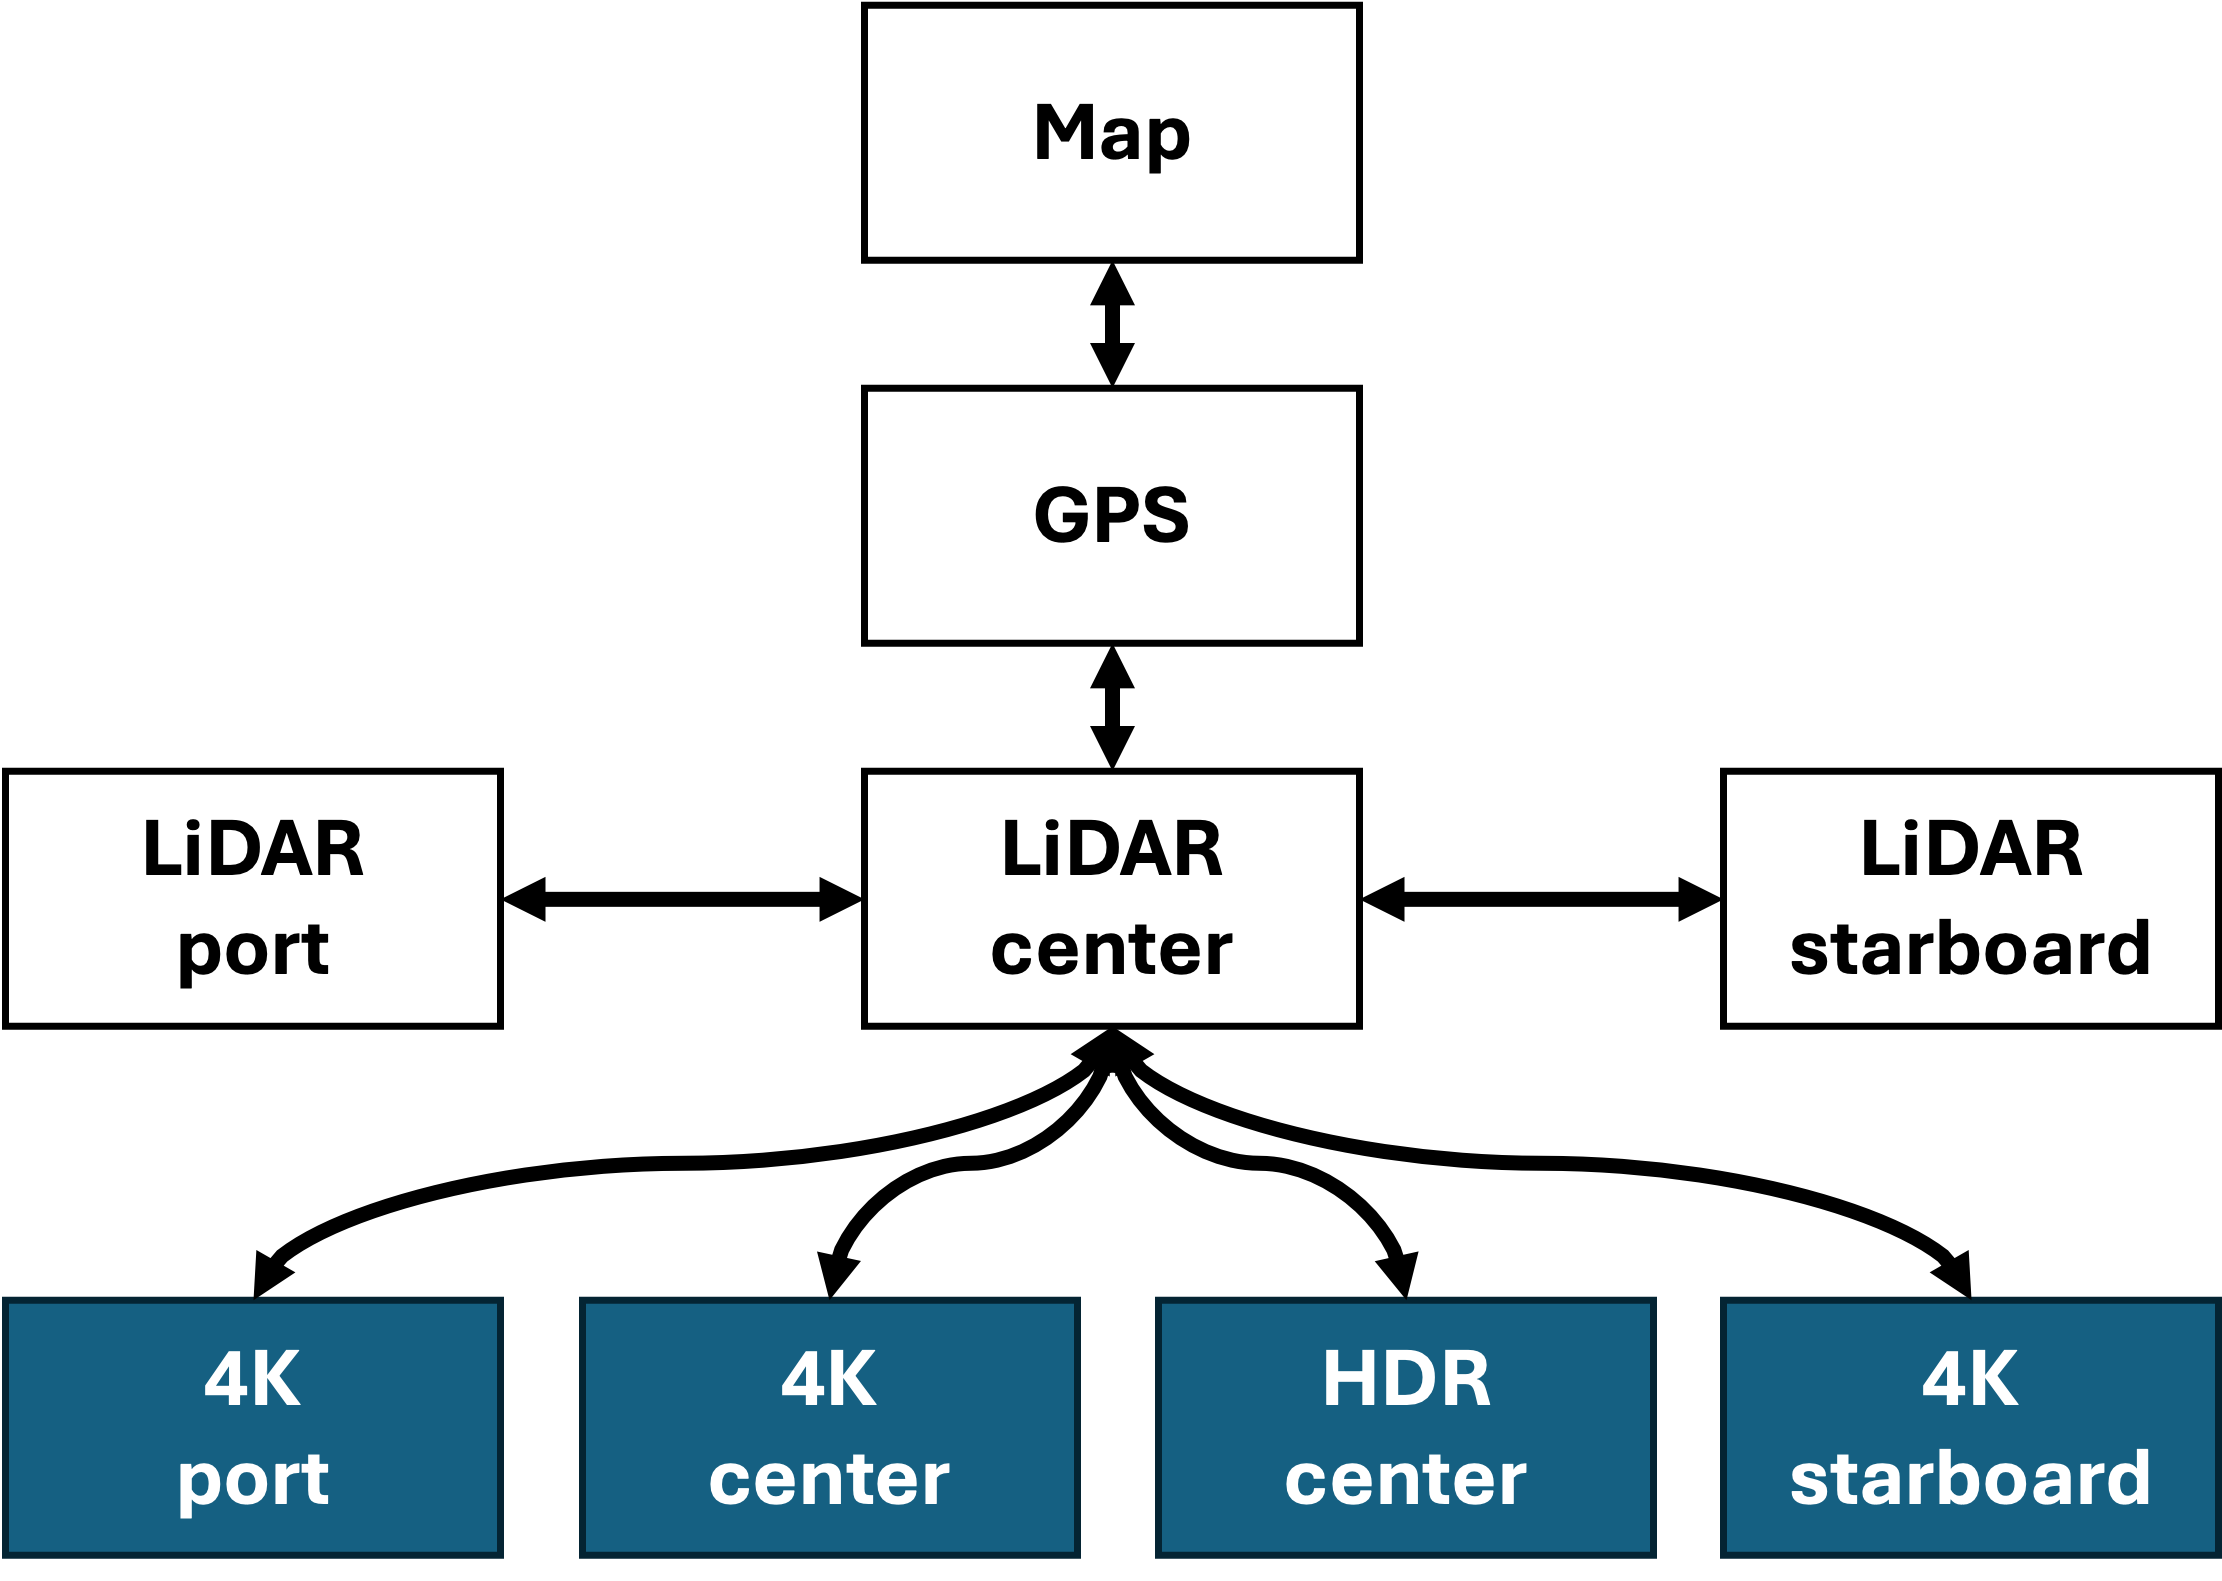
\includegraphics[width=0.7\linewidth]{Images/tf_tree_1.png}
    \caption{Transform hierarchy for Minion: the GPS-defined \texttt{map} frame anchors the ROS TF tree used for LiDAR–camera projection and sensor fusion.}
    \label{fig:tf_tree}
\end{figure}

%%%%%%%%%%%%%%%%%%%%%%%%%%%%%%%%%%%%%%%%%%%%%%%%%%%%%%%%%%%%%%%%%%%%
\subsection{Spatial Calibration} \label{spatial_calibration}

Before data from the camera and \ac{LiDAR} sensors can be combined, each device must be spatially calibrated through intrinsic and extrinsic transformations.  
This process establishes the geometric relationships required to express all sensor measurements in a unified coordinate frame, enabling accurate projection of \ac{LiDAR} points onto the camera image plane.

Calibration begins with determining the camera’s intrinsic parameters, followed by estimation of the extrinsic transformation that defines the rigid-body relationship between the camera and each \ac{LiDAR} sensor.  
The following sections describe the methods and results of this calibration process.

%%%%%%%%%%%%%%%%%%%%%%%%%%%%
\subsubsection{Extrinsic Calibration} \label{extrinsic_tform}
\subfile{sections/extrinsic_tform}

\begin{figure}[htbp]
    \centering
    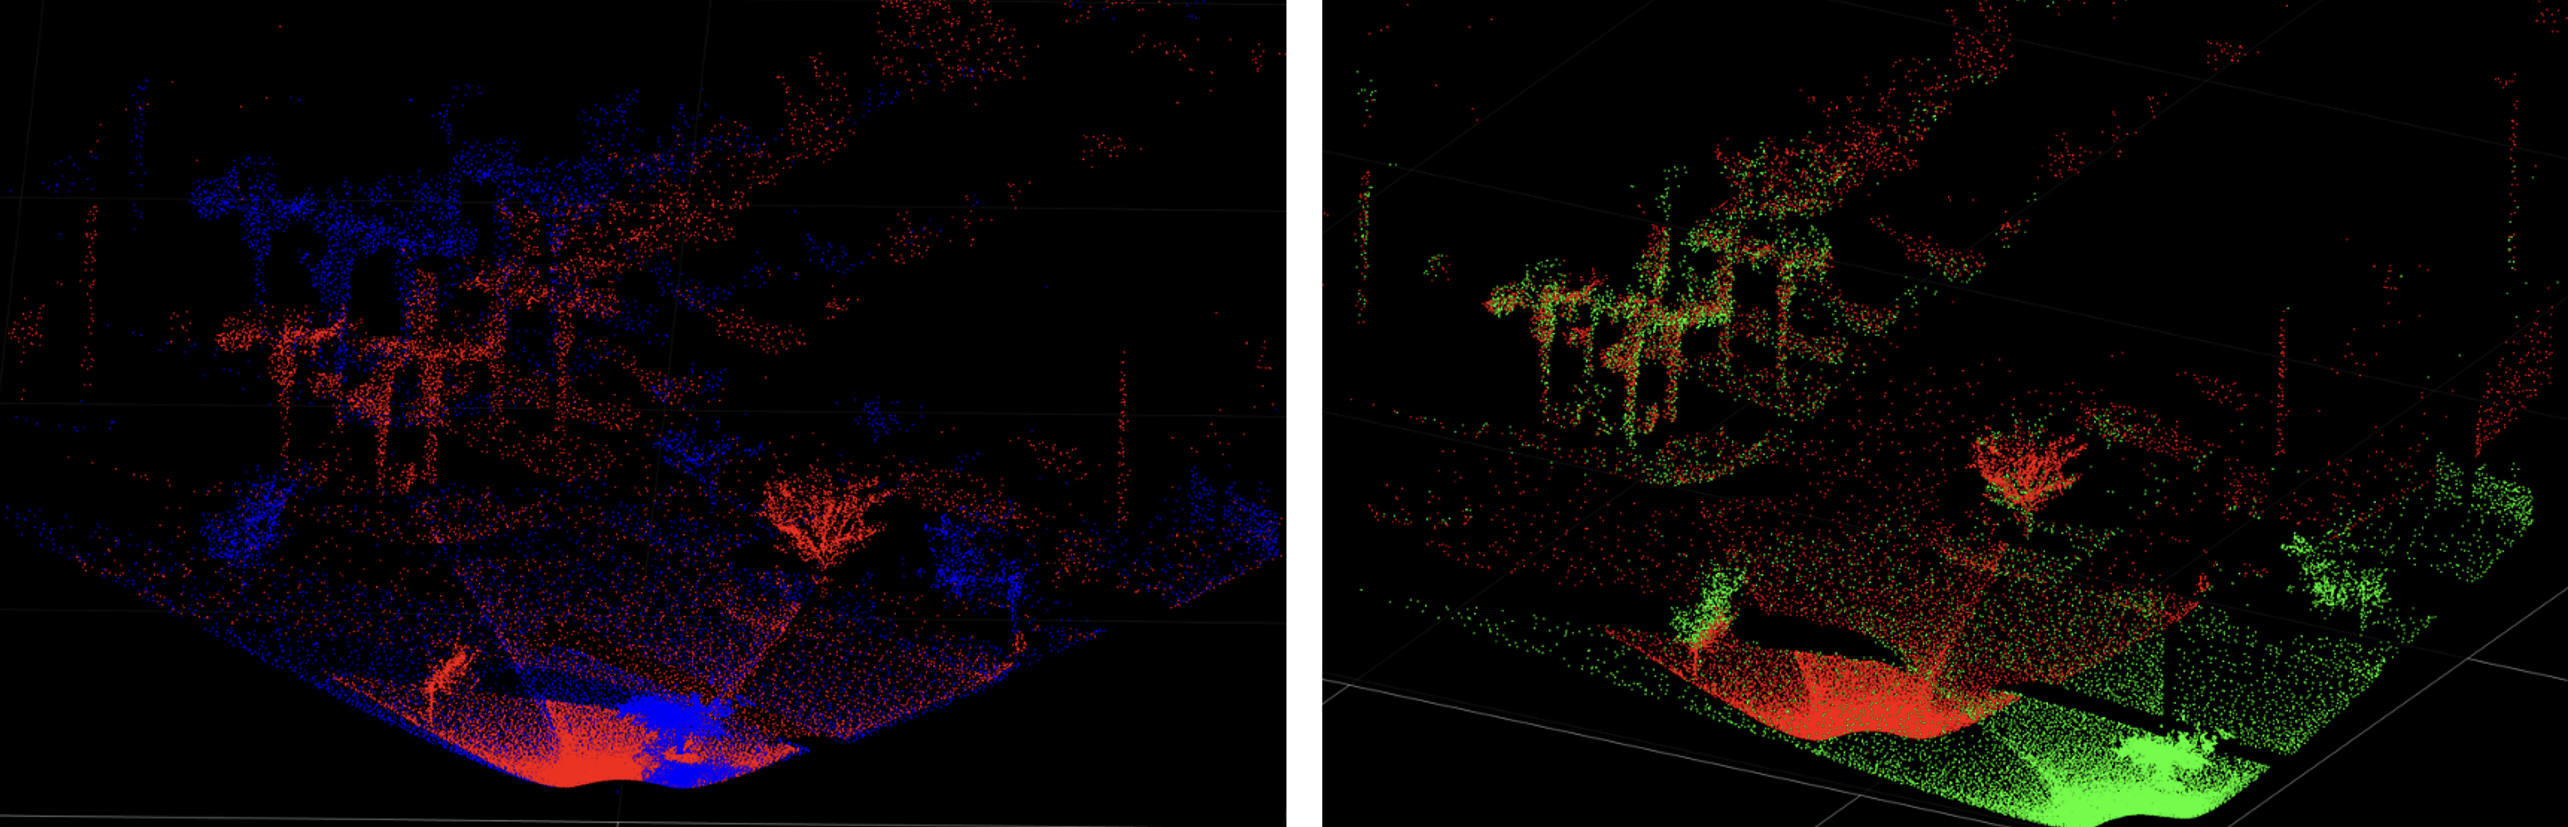
\includegraphics[width=0.9\linewidth]{Images/Lidar2Lidar.png}
    \caption{Example of LiDAR–LiDAR alignment.}
    \label{fig:Lidar2Lidar}
\end{figure}

%%%%%%%%%%%%%%%%%%%%%%%%%%%%
\subsubsection{Camera Intrinsics} \label{camera_intrinsics}
\subfile{sections/cam_intrinsics}

\begin{figure}[htbp]
\centering
\makebox[\textwidth][c]{%
    \begin{subfigure}[t]{0.3\textwidth}
        \centering
        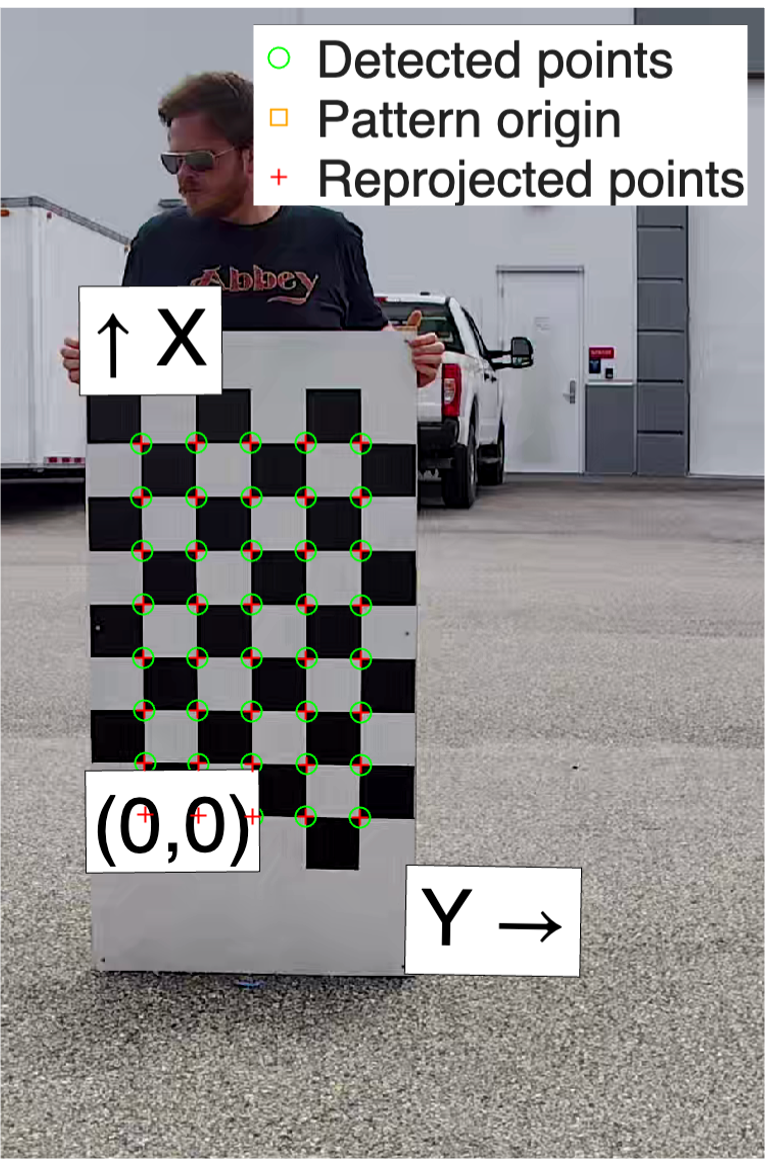
\includegraphics[width=\textwidth]{Images/cam_calib_1.png}
        \caption{A single example of detected and reprojected checkerboard corners.}
        \label{fig:cam_calib_1}
    \end{subfigure}
    \hspace{2em}
    \begin{subfigure}[t]{0.625\textwidth}
        \centering
        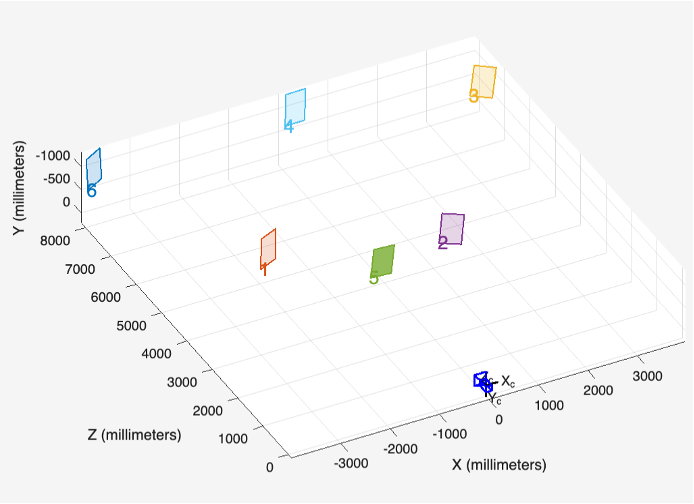
\includegraphics[width=\textwidth]{Images/cam_calib_2.png}
        \caption{Reprojection of sample target poses into the 3D world frame after calibration.}
        \label{fig:cam_calib_2}
    \end{subfigure}%
}
\caption{Checkerboard images are processed to detect corners. Agreement between detected (green circles) and reprojected (red crosses) points demonstrates corner localization and mapping of the image coordinate system.(left), which enable intrinsic parameters to be estimated and validated by reprojecting known targets into 3D space (right).}
\label{fig:cam_calib}
\end{figure}


\subsubsection{Camera to LiDAR Extrinsic Calibration} \label{camLidar_calib}
\subfile{sections/camlidar_calib}

\begin{figure}[htbp]
\centering
\makebox[\textwidth][c]{
    \begin{subfigure}[t]{0.44\textwidth}
        \centering
        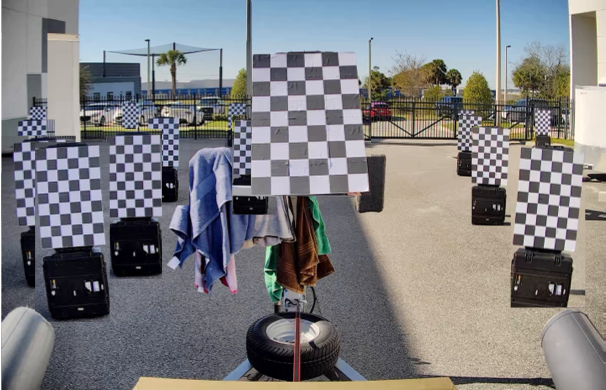
\includegraphics[width=\textwidth]{Images/checkerboard.png}
        \caption{Composite image of multiple checkerboard target locations.}
        \label{fig:checkerboard}
    \end{subfigure}
    \hspace{2em}
    \begin{subfigure}[t]{0.44\textwidth}
        \centering
        \includegraphics[width=\textwidth]{Images/LiDAR_calib.png}
        \caption{Composite of checkerboard locations in the LiDAR reference frame.}
        \label{fig:LiDAR_calib}
    \end{subfigure}
}
\caption{Checkerboard targets used for camera intrinsic (left) and LiDAR extrinsic (right) calibration. Red dots mark detected corner points transformed into the LiDAR frame using the initial extrinsic estimate.}
\label{fig:camLidar_calib}
\end{figure}

%%%%%%%%%%%%%%%%%%%%%%%%%%%%%%%%%%%%%%%%%%%%%%%%%%%
\subsection{Results: Spatial Calibration} \label{sec:spatial_calib_results}
\subsubsection{LiDAR–LiDAR Calibration} \label{results_lidarLidar_calib}
\subfile{sections/results_lidarlidar}

\begin{figure}[ht]
\centering
        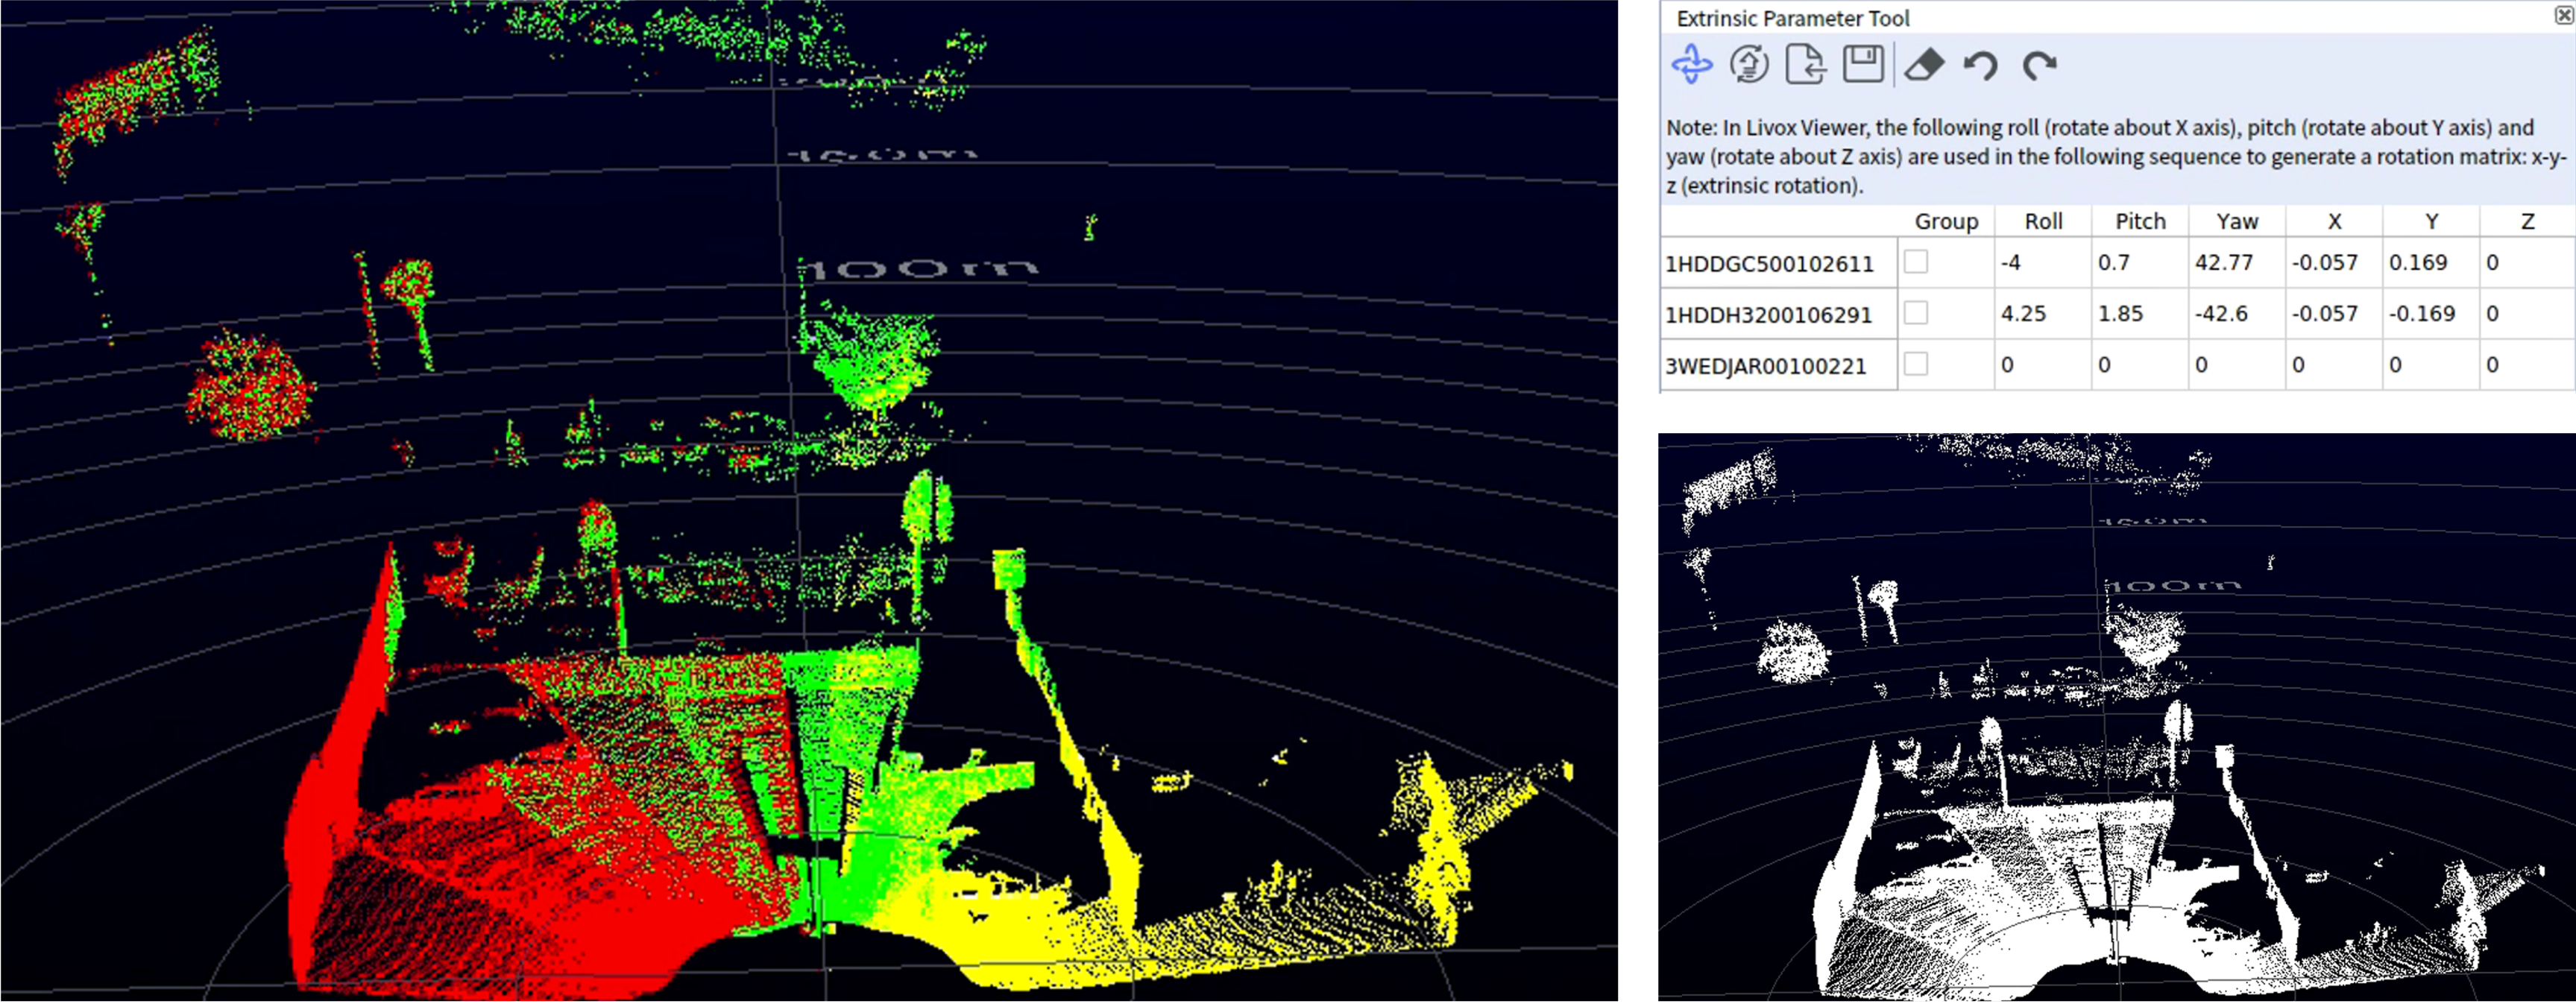
\includegraphics[width=0.95\textwidth]{Images/livox_viewer.png} 
\caption{Data from port (red), center (green), and starboard (yellow) Livox Units as viewed within the Livox Viewer software (left), and the integrated calibration tool with estimated extrinsic parameters shown (right). }
\label{fig:LidarLidar_calib}
\end{figure}

\subsubsection{Camera Calibration} \label{sec:camera_intriniscs_results}
\subfile{sections/cam_intrinsics}

\begin{figure}[htbp]
    \centering
    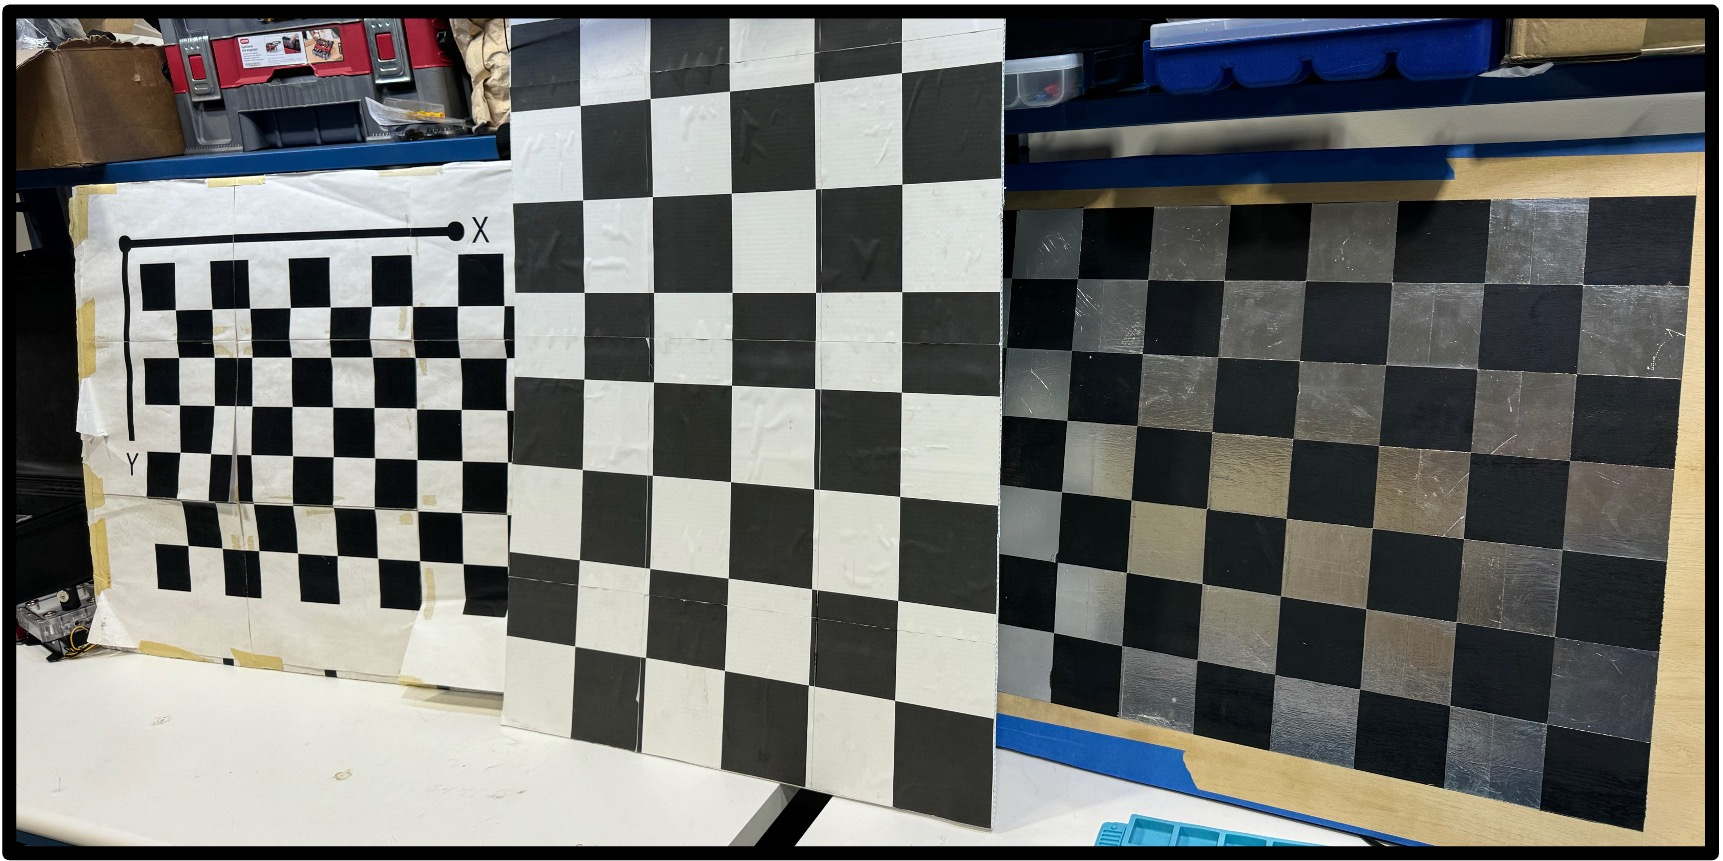
\includegraphics[width=0.9\linewidth]{Images/checkerboard_old.jpg}
    \caption{Older paper-based checkerboards maintained dimensional accuracy but degraded over time.}
    \label{fig:checkerboard_old}
\end{figure}

\begin{figure}[htbp]
    \centering
    \includegraphics[width=0.9\linewidth]{Images/Checkerboard_new.png}
    \caption{New precision-painted checkerboard target used for intrinsic calibration.}
    \label{fig:checkerboard_new}
\end{figure}

\begin{figure}[htbp]
    \centering
    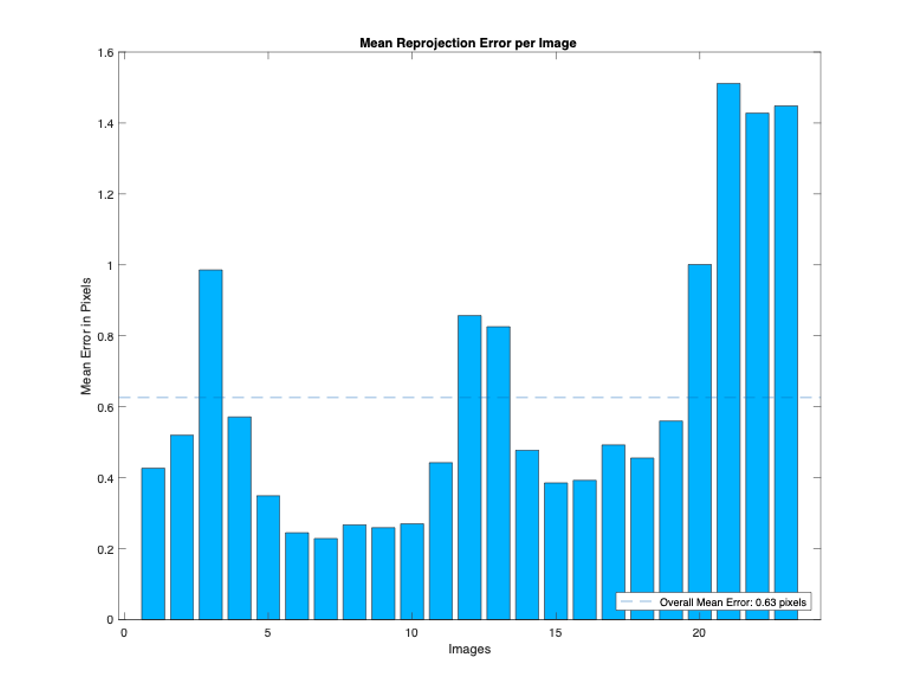
\includegraphics[width=0.9\linewidth]{Images/HDR_calib_error.png}
    \caption{Initial HDR camera calibration yielded a mean re-projection error of 0.63~pixels across the dataset.\textcolor{red}{reproduce graphic with larger text and landscape orientation. no need for square aspect ratio.}}
    \label{fig:HDR_calib_error}
\end{figure}

\subsubsection{Camera–LiDAR Calibration} \label{sec:camera-lidar_results}
\subfile{sections/results_camera-lidar}

\begin{figure}[htbp]
    \centering
    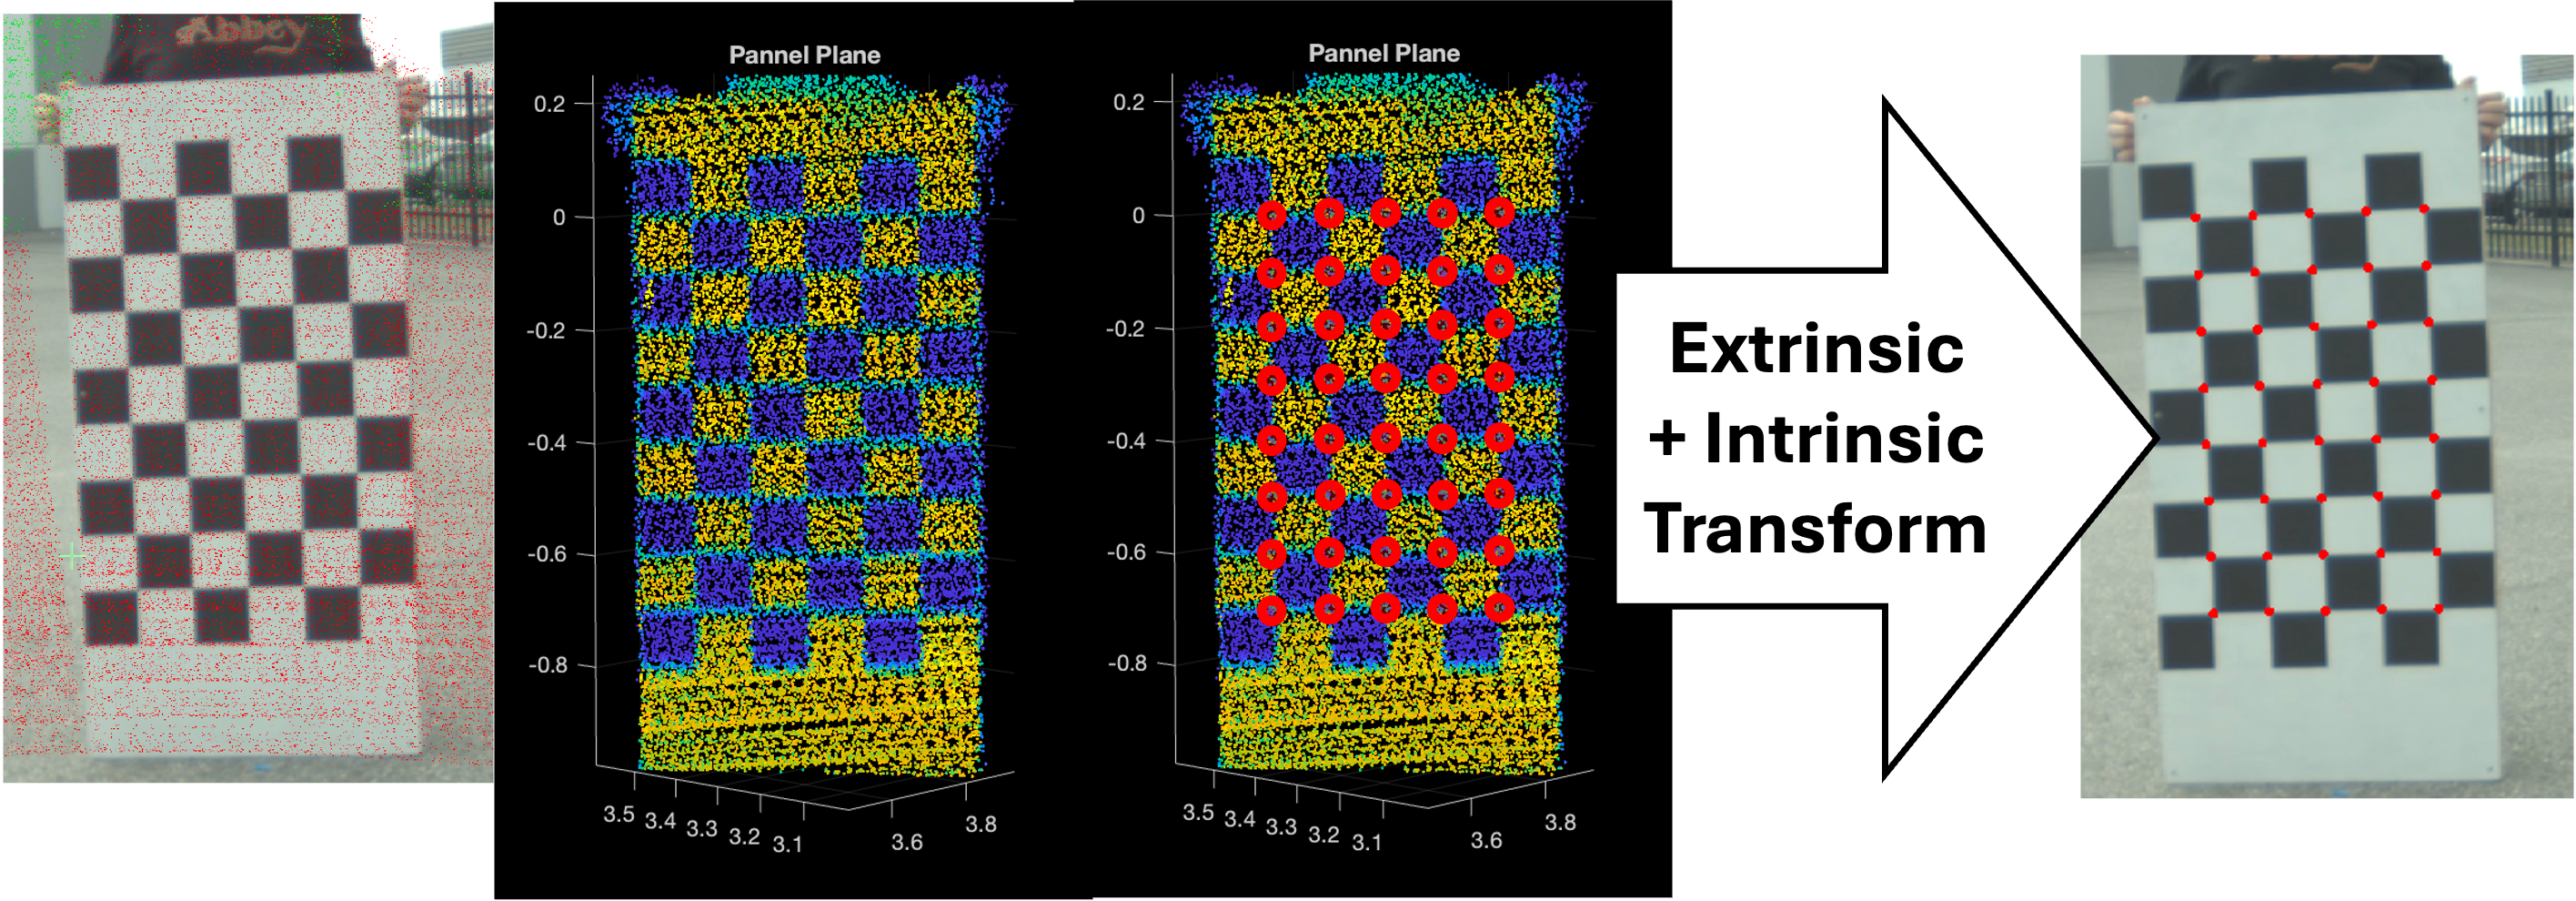
\includegraphics[width=0.8\linewidth]{Images/calib_checkers.png}
    \caption{Example of matched LiDAR point cloud and camera checkerboard detections used for extrinsic calibration.}
    \label{fig:calib_check}
\end{figure}

\begin{figure}[htp]
\begin{subfigure}{\textwidth}
\centering
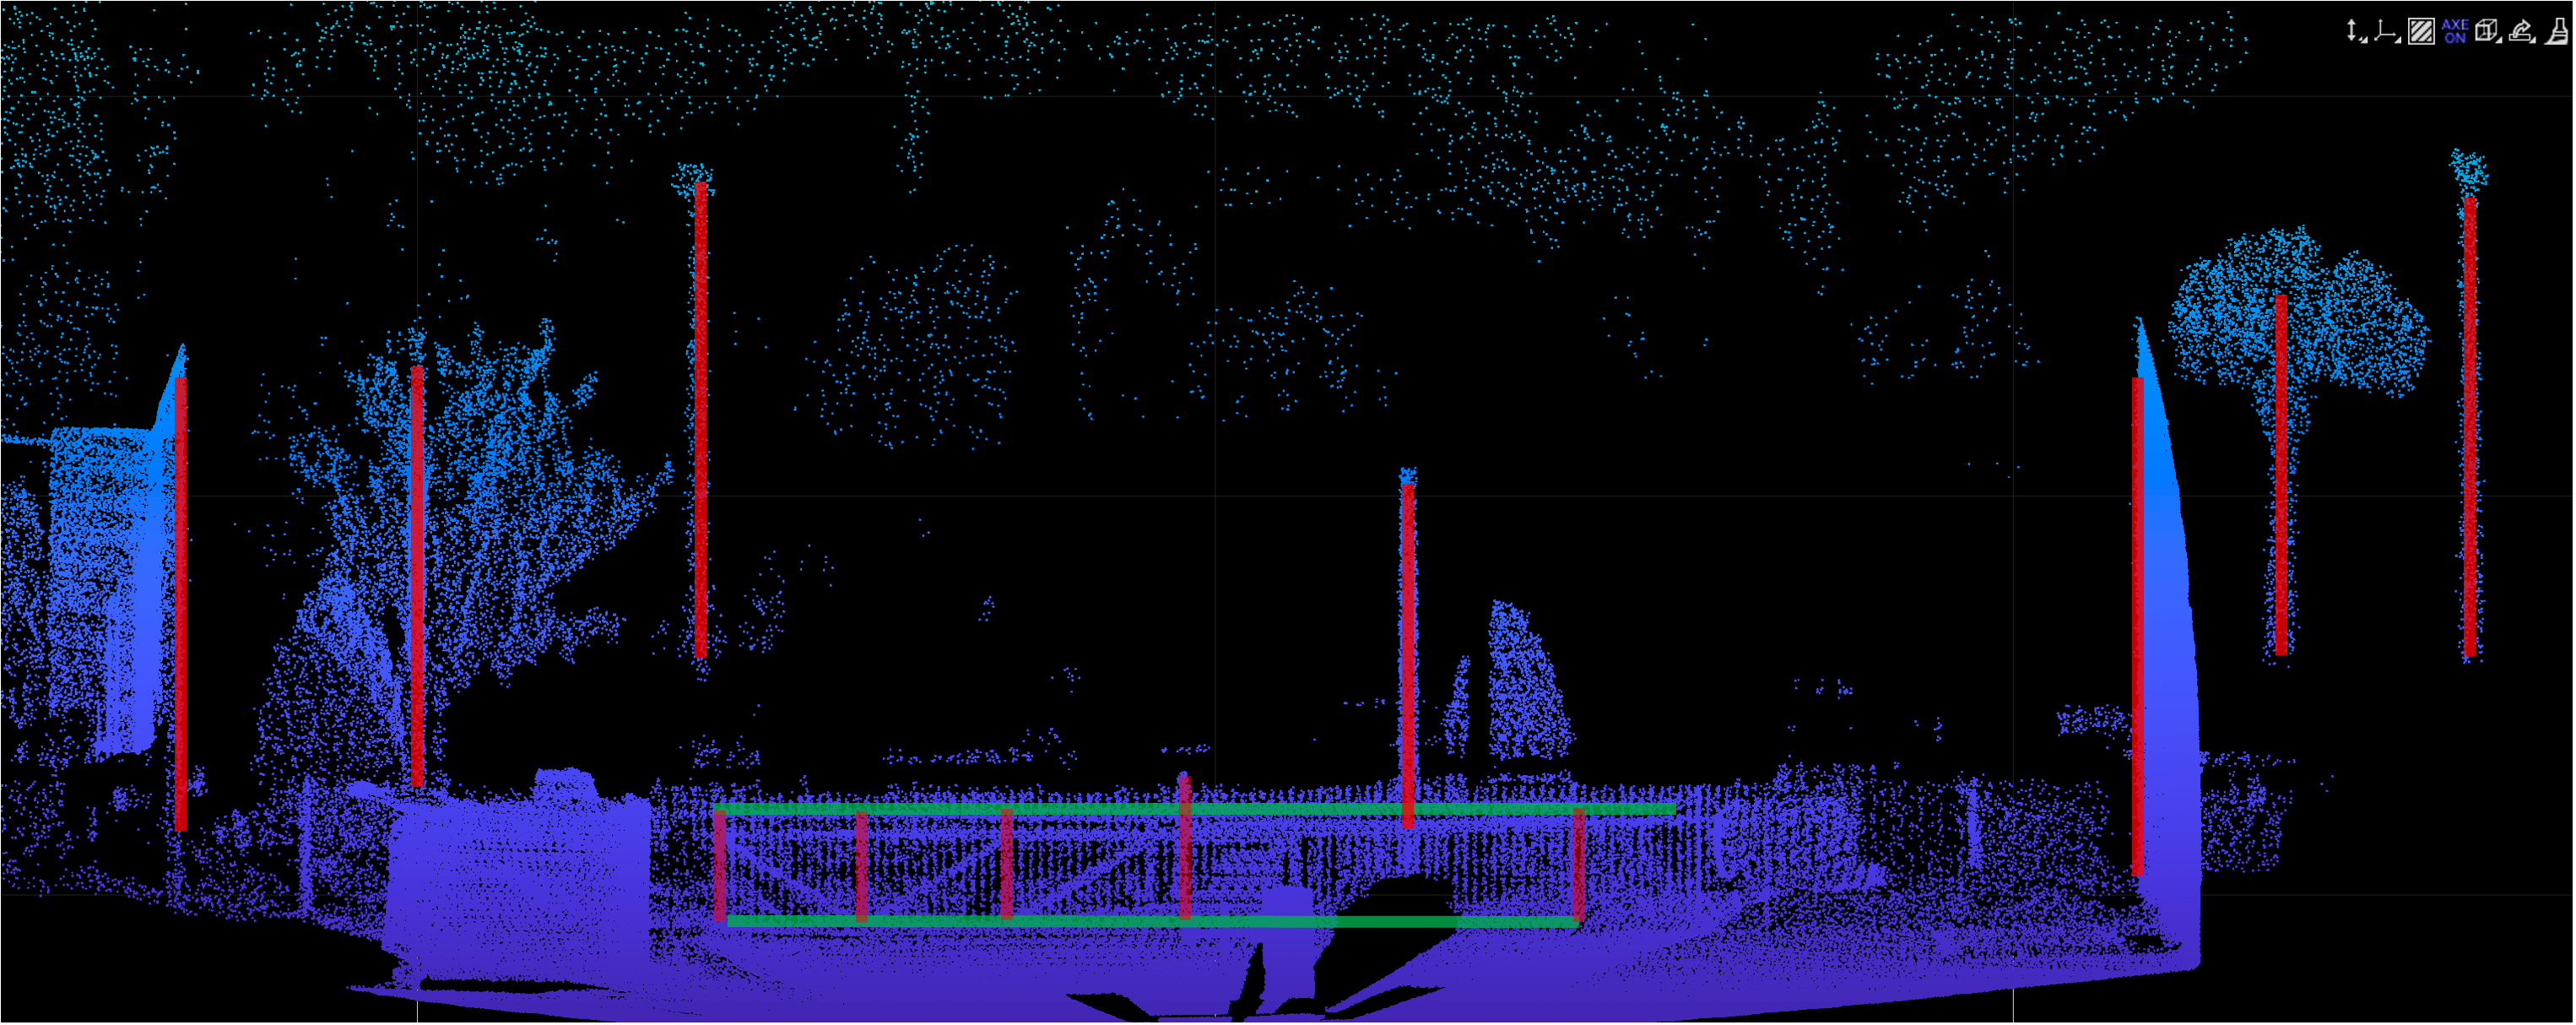
\includegraphics[width=0.94\linewidth]{Images/LiDAR_features.png}
    \caption{}
\end{subfigure}
\bigskip
\begin{subfigure}{\textwidth}
\centering
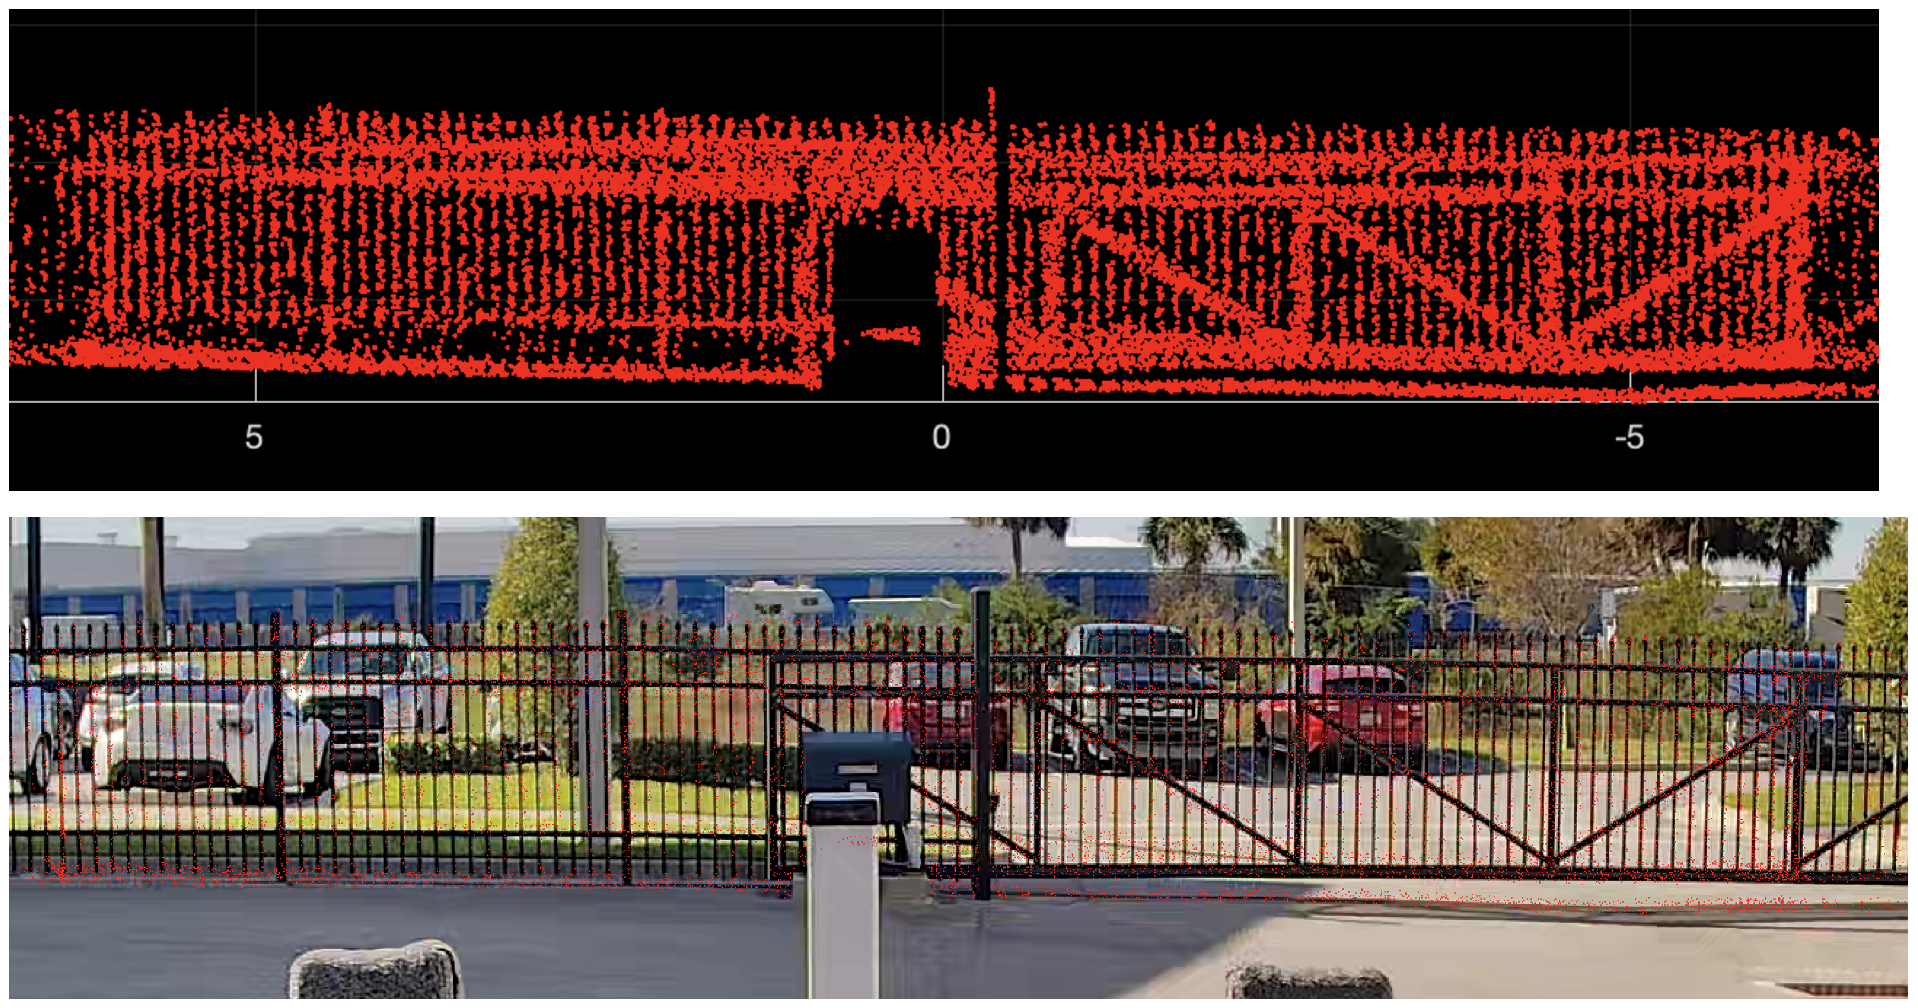
\includegraphics[width=0.94\linewidth]{Images/LiDAR_calib_fence.png}
    \caption{}
\end{subfigure}
\caption{Vertical (red) and horizontal (green) macro-level features within the point cloud (a) are isolated (b) to support visual refinement of the camera–LiDAR alignment.}
\end{figure}

\begin{figure}[ht]
    \centering
    \includegraphics[width=0.8\linewidth]{Images/LiDAR_overlay4.png}
    \caption{Initial calibration result showing early ROI-based alignment with overlaid geometric guides for evaluation.}
    \label{fig:LiDAR_overlay4}
\end{figure}
\begin{figure}[htp]
\begin{subfigure}{\textwidth}
\centering
\includegraphics[width=0.94\linewidth]{Images/LiDAR_overlay3A.png}
    \caption{Three isolated regions of interest (ROI) in the LiDAR point cloud.}
    \label{fig:LiDAR_overlay3A}
\end{subfigure}
\bigskip
\begin{subfigure}{\textwidth}
\centering
\includegraphics[width=0.94\linewidth]{Images/LiDAR_overlay3B.png}
    \caption{}
    \label{fig:LiDAR_overlay3B.png}
\end{subfigure}
\caption{Final camera–LiDAR calibration. LiDAR ROIs containing identifiable geometry (a) are projected as red pixels onto the HDR image (b) to confirm alignment quality.}
\label{HDR_calib_final}
\end{figure}

\subsection{Temporal Calibration} \label{time_sync}
\subfile{sections/time_sync}

\subsubsection{Camera Synchronization} \label{time_sync_cam}
\subfile{sections/time_sync_cam}

\subsubsection{Network Synchronization} \label{time_sync_lan}
\subfile{sections/lan_sync}

\subsection{Results: Temporal Synchronization} \label{results_time_sync_cam}
\subfile{sections/results_time_sync}

\section{Sensor Data and Dataset} \label{sec:sensor_data_dataset}
\subfile{sections/sensor_data}



%%%%%%%%%%%%%%%%%%%%%%%%%%%%%%%%%%%%%%%%%%%%%%%%%%%
%%%%%%%%%%%%%%%%%%%%%%%%%%%%%%%%%%%%%%%%%%%%%%%%%%%
%%%%%%%%%%%%%%%%%%%%%%%%%%%%%%%%%%%%%%%%%%%%%%%%%%%
\chapter{Real-time Object Detection} \label{realtime_object_detection}
% \subfile{sections/real_time_obj_det}
% % a brief introduction to the chapter and overview of model selection prior to method description
% % 2 to 3 paragraphs

% \section{YOLO} \label{yolo}
% \subfile{sections/yolo}
% % This section only discusses the methods used for the YOLO object detection. 
% % 3 to 4 paragraphs

% %%%%%%%%%%%%%%%%%%%%%%%%%%%%%%%%%%%%%%%%%%%%%%%%%%%%%%%%%%%%%%
% \subsection{YOLO Training Data} \label{sec:yolo_training_data}
% % \subfile{sections/training_data_yolo}






% \section{GB-CACHE} \label{gbcache}
% \subfile{sections/gbcache}
% % This section only discusses the methods used for the GB-CACHE object detection.
% % 3 to 4 paragraphs

% \subsection{GB-CACHE Training Data} \label{training_data_gbcache}
% % \subfile{sections/training_data_gbcache}

% \section{Classification Results} \label{sec:classify}
% \subfile{sections/sec:classify}

% \subsection{YOLO Performance} \label{performance_yolo}
% \subfile{sections/performance_yolo}

% \subsection{GB-CACHE Performance} \label{performance_gbcache}
% \subfile{sections/performance_gbcache}

% \subsection{Feature Relevance} \label{features_gbcache}
% \subfile{sections/features_gbcache}

% \begin{figure}
%     \centering
%     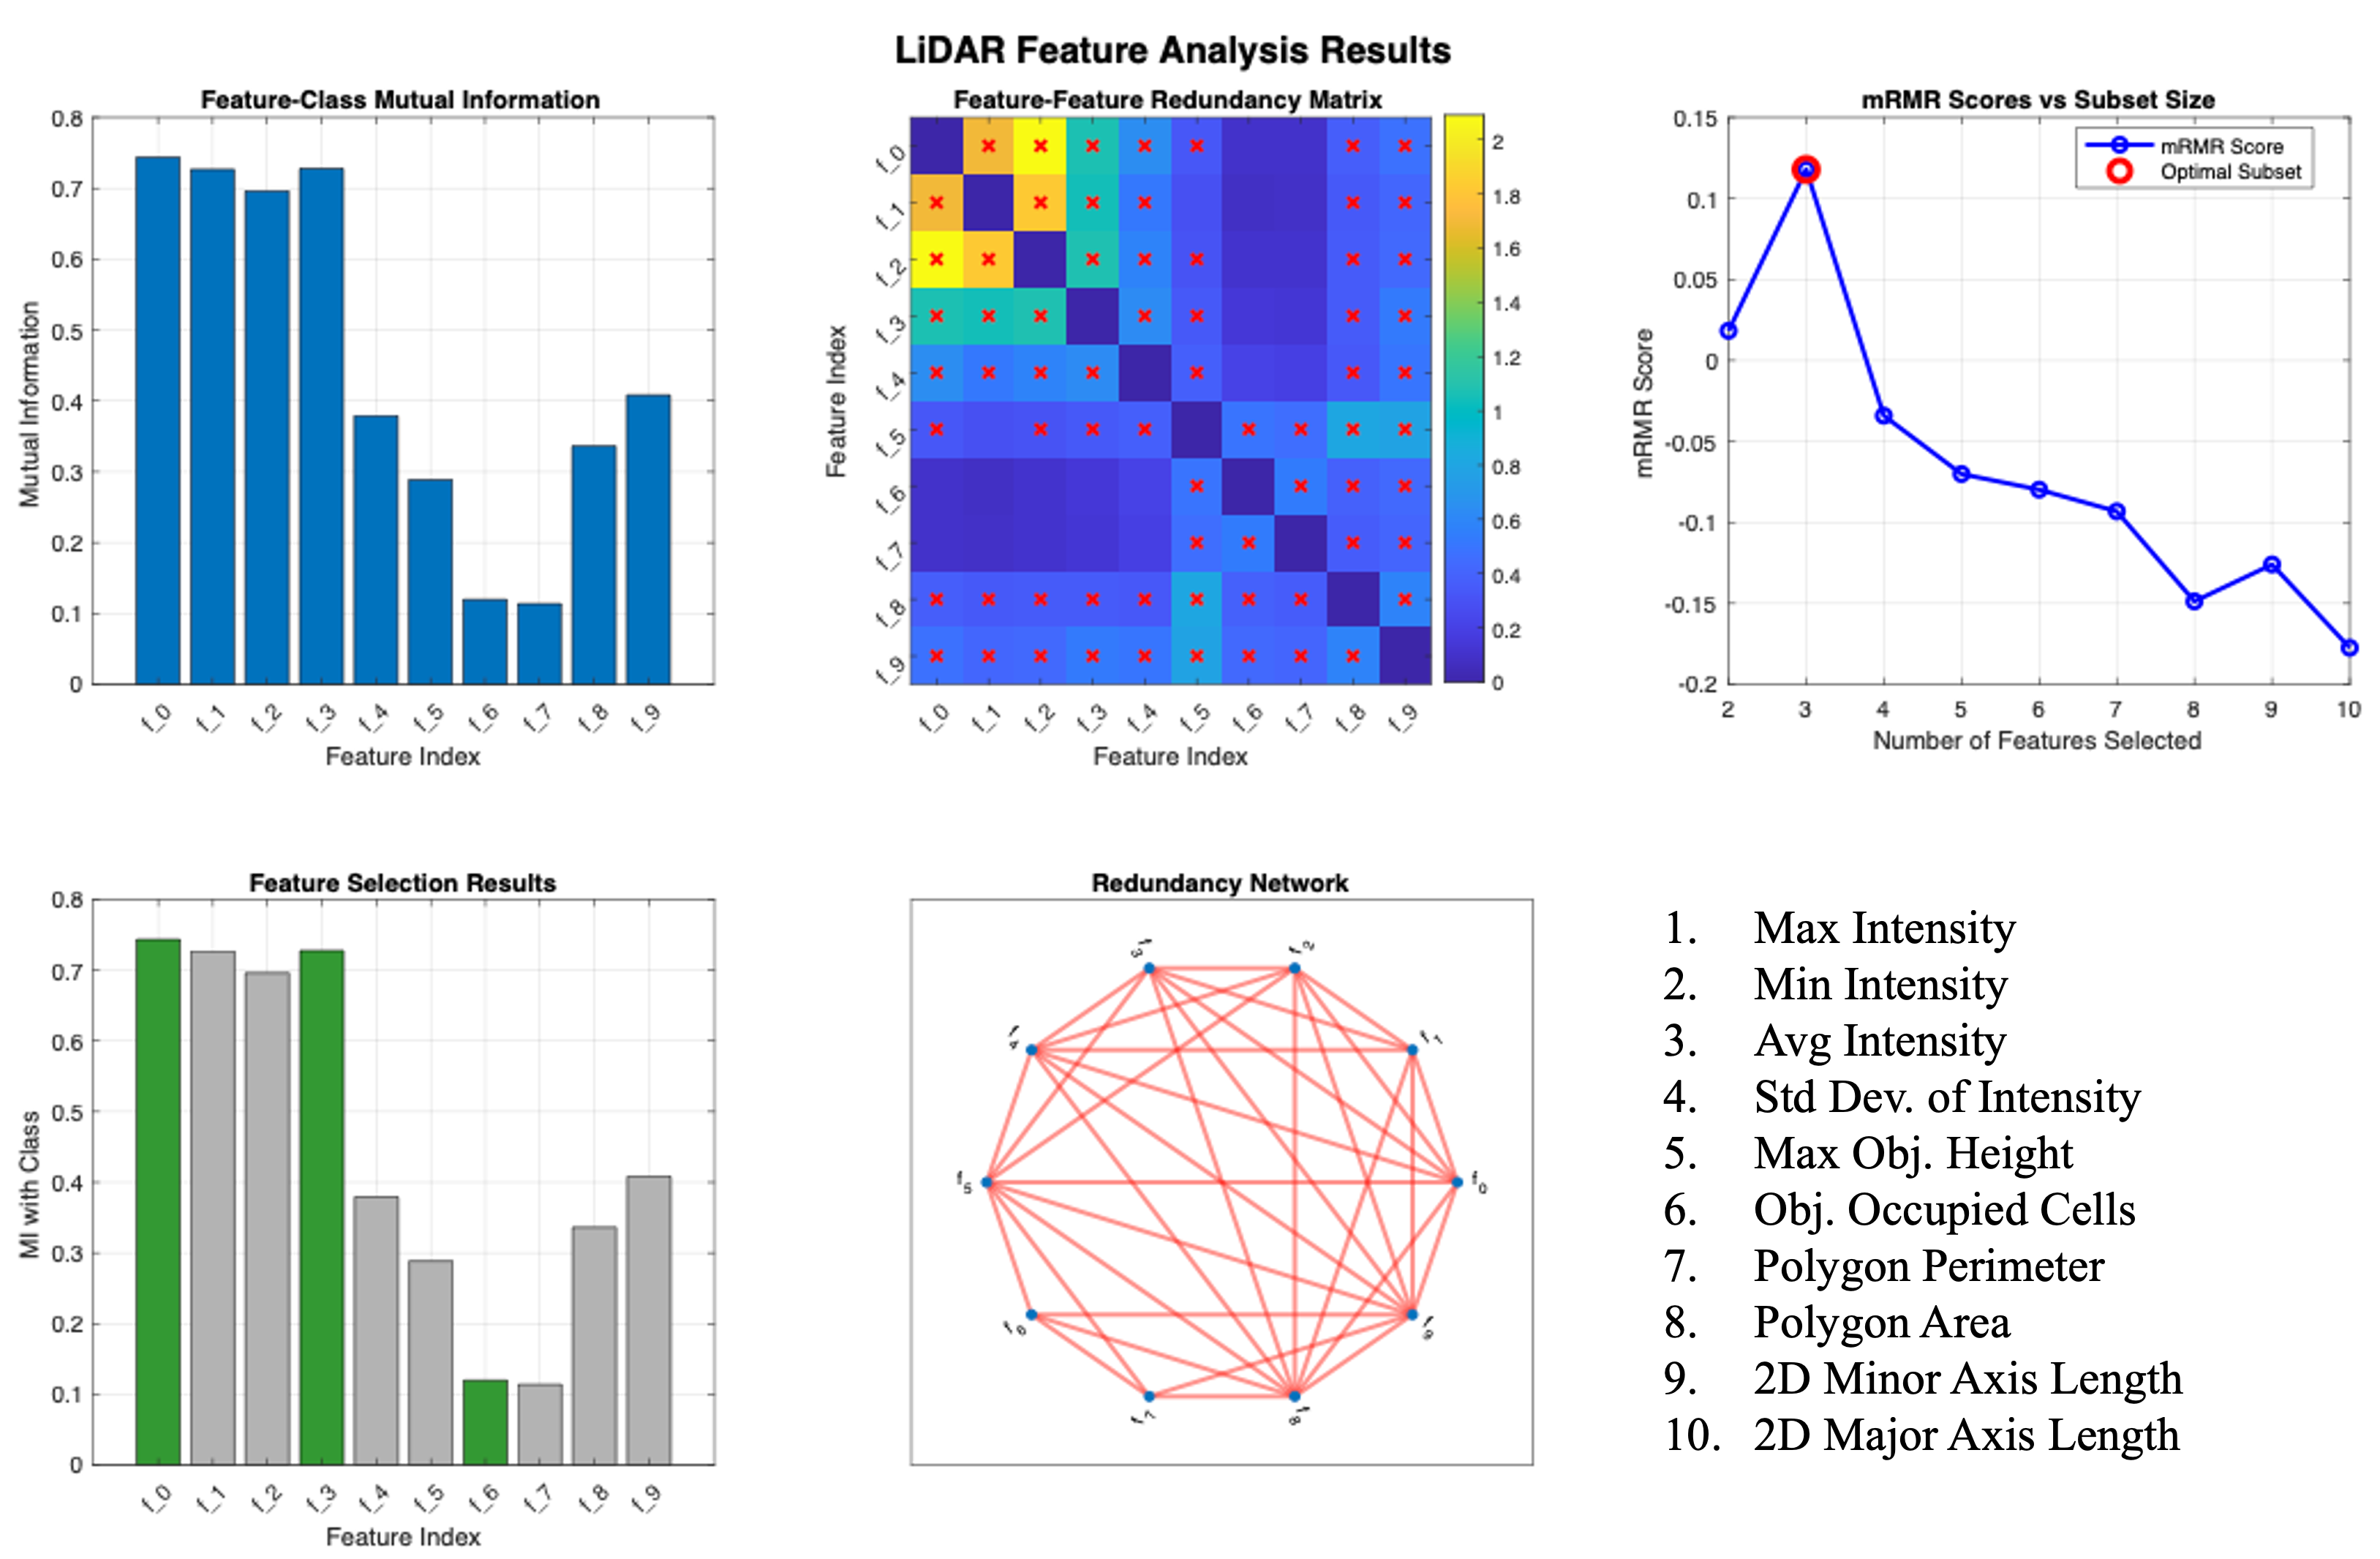
\includegraphics[width=0.95\linewidth]{Images/MI_analysis.png}
%     \caption{Caption}
%     \label{fig:MI_analysis}
% \end{figure}

% \begin{figure}
%     \centering
%     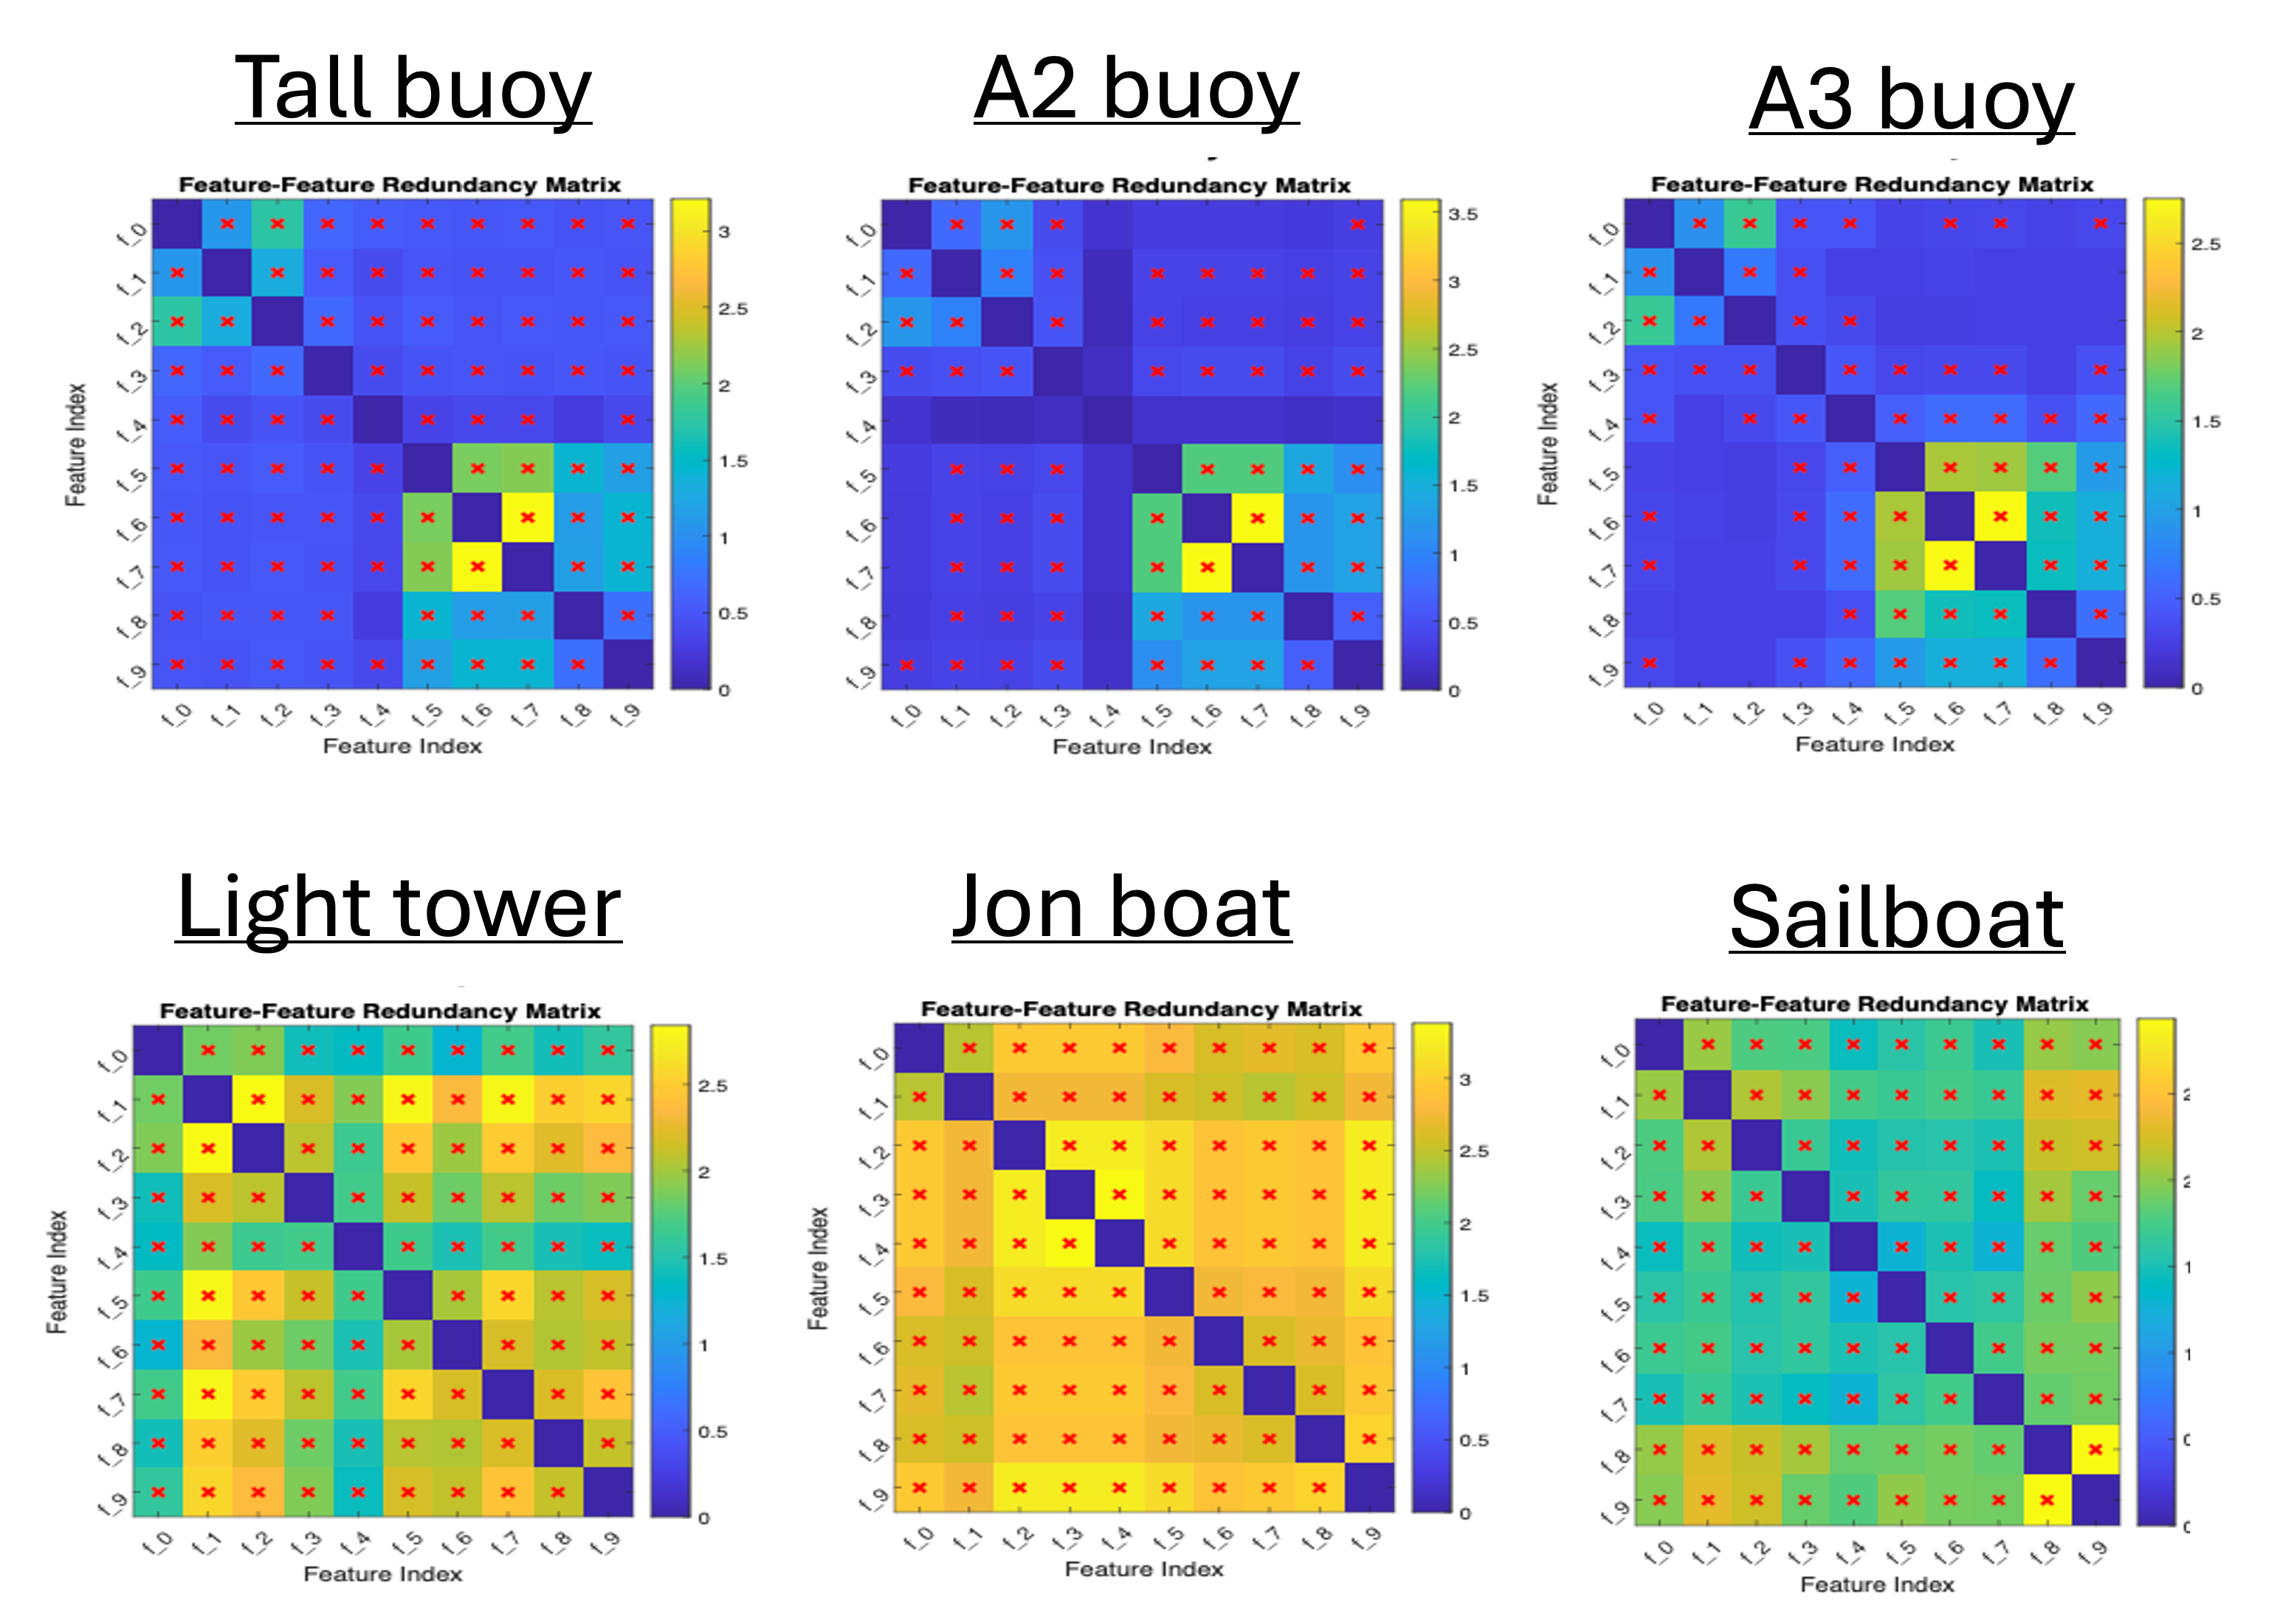
\includegraphics[width=0.95\linewidth]{Images/MI_pairwise.png}
%     \caption{Caption}
%     \label{fig:MI_pairwise}
% \end{figure}

% \section{Detection Results} \label{detect_results}
% \subfile{sections/detect_results}

% \section{Late Fusion} \label{fusion}
% \subfile{sections/fusion}
% % This section only discusses the methods used for the late fusion object detection. 

% % \section{Model Performance} \label{performance}
% % \subfile{sections/performance}
% % This section will hold all results from analysis from the YOLO, GB cache, and late fusion techniques. 



Real-time object detection lies at the core of autonomous perception, enabling vehicles to interpret their surroundings and respond safely to dynamic environments.
Effective detection requires identifying, classifying, and localizing objects rapidly enough to support decision-making and control loops, often under constraints of limited onboard computing and bandwidth.
In this work, these challenges are examined through vision and LiDAR detection pipelines implemented on the Minion sensing platform.

The central focus of this investigation is the development of a late-fusion framework that integrates information from both sensing domains to enhance detection robustness and confidence.
This framework represents the primary contribution of the research and demonstrates how visual and LiDAR detections can be combined at the decision level to exploit the complementary strengths of each sensing modality while mitigating their individual limitations.

To establish a meaningful basis for evaluation, two single-modality detection systems were selected as comparative baselines.
YOLOv8 represents the class of data-driven neural network detectors optimized for vision-based perception, while GB-CACHE represents the class of deterministic, geometry-based algorithms used for LiDAR clustering and segmentation.
These methods were not chosen to exhaust all available detection approaches, but because they are broadly representative of the state of the art within their respective sensing domains.

YOLOv8 was selected for its status as one of the most widely adopted and optimized real-time vision networks, capable of achieving high detection accuracy and efficient inference on GPU-based platforms.
Its inclusion provides a mature and well-understood benchmark for camera-based perception and a reliable reference for evaluating the complementary benefits of late fusion.

GB-CACHE was selected as a deterministic counterpart to YOLO that performs real-time clustering and segmentation without the computational overhead or data dependency of neural network–based LiDAR methods.
Its use of concave-hull extraction provides boundary representations more meaningful for maritime navigation than the simplified 3D bounding boxes produced by models such as PointNet or VoxelNet.
This geometry-driven approach broadens the scope of the comparative study, especially given that the advantages of neural LiDAR methods for real-time deployment remain unproven.

These two approaches represent two distinct strategies for real-time perception, and the late-fusion method developed in this work integrates their complementary strengths to achieve higher confidence detections across a range of operating conditions.
The following sections examine each detection method in sequence.
Section~\ref{yolo} presents the YOLOv8 vision-based detector and its implementation for real-time object recognition.
Section~\ref{gbcache} describes the GB-CACHE algorithm for LiDAR-based clustering and object segmentation.
Finally, Section~\ref{fusion} introduces the late-fusion framework developed in this research and evaluates its performance relative to the single-modality detectors through a comparative analysis of detection accuracy, computational efficiency, and real-time operation.

%%%%%%%%%%%%%%%%%%%%%%%%%%%%%%%%%%%%%%%%%%%%%%%%%%%%%%%%
\section{YOLO} \label{yolo}

% Purpose and Context
The eighth generation of the \ac{YOLO} object detection framework developed by Ultralytics was selected to provide a high-performance, real-time vision baseline for this research. 
% \textcolor{red}{add something about semantic and information-rich data?}
This method of detection gained popularity for its ease of use and implementation for detecting and localizing objects within an image.
Once an object is detected, the pixel coordinates it occupies within the image frame is bounded with a rectangle known as the bounding box (see Figure \ref{fig:YOLO_tower}).
Its open-source models are pretrained on the COCO dataset, a large repository containing approximately 1.5 million labeled images, and are provided in various sizes and qualities, which can be deployed on a wide variety of edge computing hardware.
Additionally, transfer learning is simple to apply, allowing these models to be tailored for more specific use cases, such as maritime environments.

\begin{figure}
    \centering
    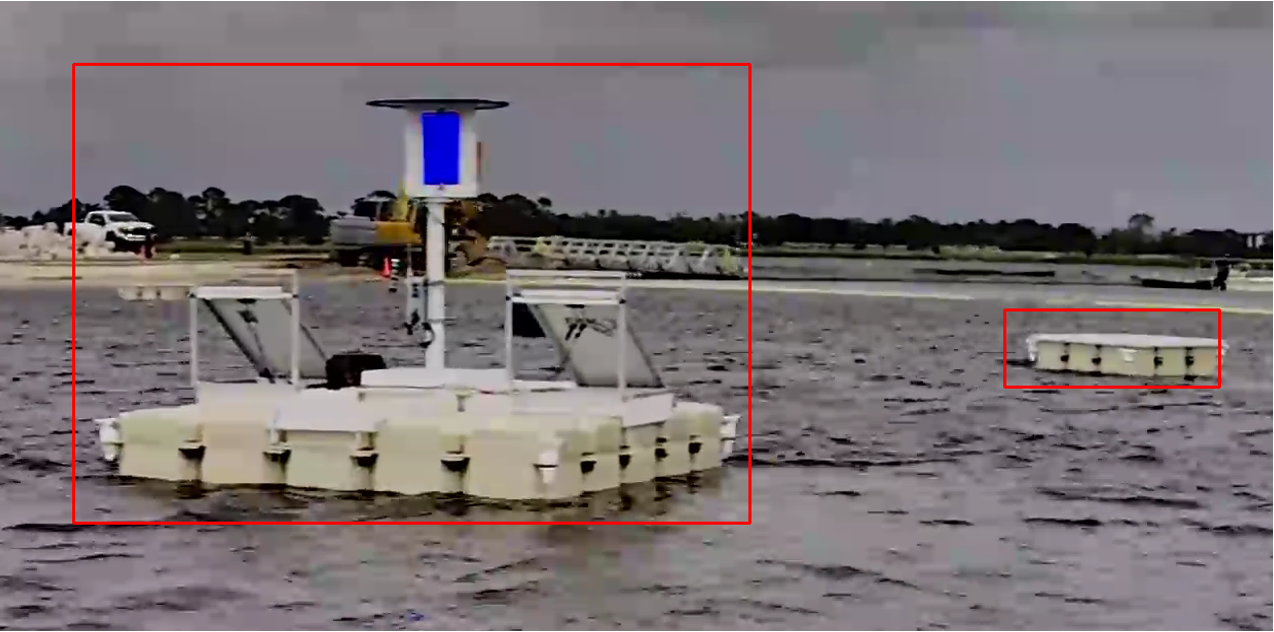
\includegraphics[width=0.75\linewidth]{Images/YOLO_ex1.png}
    \caption{Rectangular bounding boxes placed around maritime objects detected by a re-trained YOLO detection model.}
    \label{fig:YOLO_tower}
\end{figure}

The name YOLO refers to the one-shot convolutional neural network utilized to perform both detection and localization in a single pass of the network.
This architecture is what makes it fast, and for real-time object detection applications. 
Before the release of version 8 in 2023, the dual action of detection and localization required that the location and dimension of the bounding box also had to be encoded into the model.
Version 8 was the first to utilize dual-detection heads at the end of the CNN.
The first detection head identifies if and where an object is present within the image, and the second is used to determine the bounding box for the object.
This "anchor-free" architectural change not only makes localization of the detected objects more reliable, but also alleviates some of the intense transfer learning burden that was required for fine-tuning the pretrained models in earlier versions \cite{ultralytics}.

The widespread adoption of YOLOv8 and the fundamental architectural changes in this version make it the optimal choice to provide a baseline visual detection method.
% However, this mode of detection is not without its compromises, \textcolor{red}{as will be detailed in Section ____.}



% The YOLO Framework
% Describe the principle succinctly:

% YOLOv8 Architecture
% This section should flow from general framework to version-specific improvements:

% Image Resolution and Input Scaling
% Transition to operational detail and experimental consistency:

% Detection Scale and Spatial Sensitivity
% Discuss how feature maps relate to the detection limit:

% Model Constraints and Applicability
% Then note practical limitations and their relevance:

% Implications for Real-Time Fusion
% Conclude the section by connecting to your larger research goal:

% \textcolor{red}{To establish a performance baseline for real-time, vision-based object detection, this study employed the You Only Look Once (YOLO) framework, a single-stage convolutional neural network (CNN) architecture designed for end-to-end detection and classification. Unlike two-stage detectors that separately generate region proposals before classification, YOLO formulates detection as a direct regression problem, predicting bounding box coordinates and class probabilities simultaneously. This design allows all detections to occur in a single computational pass, providing the speed necessary for autonomous and embedded sensing applications. The visual detection results presented here serve as the reference modality for comparison with LiDAR-based detection methods and for evaluating computational performance in the subsequent late-fusion framework.}

% \textcolor{red}{
% The eighth-generation YOLOv8 model developed by Ultralytics was selected due to its stability, active development, and high inference efficiency on modern hardware. YOLOv8 integrates several architectural refinements that enhance accuracy and convergence speed relative to previous versions. The model employs an anchor-free detection strategy, eliminating the predefined bounding-box templates that characterized earlier YOLO iterations. Instead, YOLOv8 predicts the object center, width, and height directly, simplifying configuration and improving adaptability to objects of varying aspect ratios and scales. A decoupled detection head separates the regression and classification branches of the network, allowing independent optimization of spatial and semantic components during training. The backbone of the network uses C2f (Cross-Stage Partial Fusion) modules, which improve feature reuse and gradient flow while reducing overall computation. These modifications collectively contribute to higher accuracy and reduced latency, both of which are critical for on-board real-time inference
% The model employs modern loss functions to enhance bounding-box precision. The Complete-IoU (CIoU) loss function refines localization by incorporating geometric distance and aspect ratio penalties, while the Distribution-Focal Loss (DFL) improves boundary regression stability. Together, these losses improve the correspondence between predicted and ground-truth boxes and facilitate more consistent convergence during training. The network was implemented in PyTorch using the native Ultralytics framework, which provides integrated preprocessing, data augmentation, and export utilities. This implementation enables consistent deployment across GPU-based and embedded computing platforms without manual configuration
% }
% \textcolor{red}{
% All input frames were processed at a resolution of 640 × 640 pixels, which corresponds to YOLOv8’s default operational size and the native output of the experimental imaging system. Maintaining this native resolution avoided unnecessary interpolation and ensured a one-to-one correspondence between camera pixels and network input. YOLOv8 performs detection at three spatial scales, corresponding to feature-map strides of 8, 16, and 32 pixels relative to the input. These scales allow simultaneous sensitivity to small, medium, and large objects within a single inference pass. For a 640 × 640 input image, these feature maps have effective dimensions of 80 × 80, 40 × 40, and 20 × 20 cells, respectively. Each cell in the smallest-stride feature map represents an 8 × 8 pixel region of the input image.}
% \textcolor{red}{
% Because of this multi-scale design, the network’s minimum detectable object size is bounded by the stride of the smallest feature map. Objects must occupy multiple adjacent cells to generate distinct activations; those confined to a single cell are typically lost through downsampling or non-maximal suppression. Empirical evaluation and prior literature indicate that YOLOv8 reliably detects objects approximately 16–32 pixels in width or height—roughly 0.5–1 percent of the frame area for a 640 × 640 input. Objects smaller than this threshold generally produce low-confidence or unstable detections.}
% \textcolor{red}{
% This limitation arises from several interrelated factors. First, downsampling loss in convolutional and pooling layers reduces high-frequency detail, causing very small features to disappear from deeper network layers. Second, the receptive field of later layers covers large portions of the input image, diminishing the spatial specificity required for fine-scale detections. Third, training bias inherent to datasets such as COCO and VOC, which contain relatively large annotated objects, restricts the network’s learned sensitivity to sub-pixel features. These factors collectively define the lower bound of object detectability in standard YOLOv8 configurations.}
% \textcolor{red}{
% The 640 × 640 camera used in this study matches the network’s native input dimension, permitting direct inference without rescaling and ensuring consistent timing measurements for real-time operation. This configuration provides an accurate representation of YOLOv8’s performance under embedded deployment conditions and serves as a visual-only detection baseline against which LiDAR-based methods and fused detection results are compared in later sections. The analysis presented here therefore defines the temporal and computational characteristics of the visual detection pipeline that underpin the late-fusion approach adopted in this research.
% }


%%%%%%%%%%%%%%%%%%%%%%%%%%%%%%%%%%%%%%%%%%%%%%%%%%%%%%%%
\subsection{YOLO Training Data} \label{sec:yolo_training_data}

A manually labeled image dataset was constructed to support the transfer learning and evaluation of the YOLO object detection network. 
All YOLO training images were obtained from video recorded directly on the Jetson.
Rosbag data was recorded intermittently, whereas the cameras operated and streamed continuously.
This ensured that a large pool of video data remained separate from the main dataset and available for YOLO training.

The complete dataset contained 778 annotated images with a total of 1934 labeled maritime objects from the six classes defined in Table \ref{tab:class_map} 
Each annotation was produced through a manual labeling process for objects present within each 2880 $\times$ 860 frame. 

The final dataset contained 778 annotated images and 1934 labeled maritime objects. 
Data were divided into training, validation, and test subsets following a 70:20:10 ratio.
Each subset preserved the relative class proportions observed in the complete dataset, which contained an average of 2.5 labeled objects per image across the five categories listed in Table~\ref{tab:class_map}.
The A2 and A3 buoy variants are virtually identical when viewed in isolation, as their size difference can only be inferred through comparison or with additional depth information in the image frame. 
Because YOLO operates purely on two-dimensional image data without access to spatial depth cues, there was no practical benefit to treating these as separate classes; both were therefore labeled collectively as \texttt{round\_buoy}.
% \textcolor{blue}{Based on field observations, it is likely that A2 buoys were predominantly red, green, or blue, whereas A3 and larger buoys appeared black. 
% However, since visually similar large black buoys were also observed throughout the rosbag dataset without verified size information, these classes were merged to maintain labeling consistency.}

\begin{table}[htbp]
\centering
\begin{tabular}{lccccccc}
\hline
Subset & Images & Labels & Tall Buoy & Round Buoy & Light Tower & Jon Boat & Sailboat \\
\hline
Train & 543 & 1,343 & 12.0\% & 1.4\% & 11.2\% & 15.8\% & 59.6\% \\
Validation & 158 & 390 & 14.1\% & 1.3\% & 13.1\% & 12.8\% & 58.7\% \\
Test & 77 & 201 & 16.4\% & 1.5\% & 9.5\% & 12.4\% & 59.7\% \\
\hline
Total & 778 & 1,934 &  &  &  &  &  \\
\hline
\end{tabular}
\caption{YOLO dataset composition and class distribution across training, validation, and test subsets.}
\label{table:yolo_data_split}
\end{table}

\noindent The relative consistency across all three subsets demonstrates that the temporal stratification preserved real-world object frequency while maintaining balance for training and evaluation. 
The test set was reserved exclusively for the final performance assessment described in Chapter~\ref{realtime_object_detection}.

For this research, YOLOv8 was trained on a custom maritime dataset derived from sensor recordings collected aboard the Minion platform.
The dataset includes labeled examples of navigation markers, buoys, vessels, and other relevant maritime objects captured under diverse lighting conditions, sea states, and viewing angles.
Transfer learning was employed by initializing the network with weights pre-trained on a general-purpose dataset, then fine-tuning on the maritime-specific data to adapt the model to the target domain.

Fine-tuning was conducted using the Ultralytics YOLOv8 framework. \cite{ultralytics} %, employing a combination of data augmentation techniques—including random horizontal flips, exposure shifts, and image rotations—to improve robustness under varying lighting and sea-state conditions.
% Hyperparameters such as learning rate, batch size, and the number of epochs were optimized empirically to achieve stable convergence while minimizing overfitting.
To assess the tradeoff between detection accuracy and inference speed, three YOLOv8 model size variants (YOLOv8n, YOLOv8s, and YOLOv8m) were trained using the default parameters and evaluated over a set of training epochs.
Each model’s number of trainable parameters, summarized in Table~\ref{tab:yolo_variants}, corresponds to differences in backbone depth and channel width that balance model capacity against computational efficiency.
Training was performed over multiple epochs to identify the most efficient configuration for the dataset.
The YOLOv8m model exhibited no measurable improvement in mean average precision compared to YOLOv8s, while requiring substantially greater computational resources.
The YOLOv8s model achieved full convergence within approximately 80 epochs without signs of overtraining and was therefore selected for subsequent testing and deployment.

\begin{table}[htbp]
\centering
\begin{tabular}{l c c c c}
\hline
Model & Params (M) & FPS (RTX 3090) & mAP@50 \\
\hline
YOLOv8n & 3.2 &  110 & 0.79 \\
YOLOv8s & 11.2 &  85 & 0.84 \\
YOLOv8m & 25.9 &  63 & 0.87 \\
\hline
\end{tabular}
\caption{YOLOv8 model comparison for visual detection tasks.}
\label{tab:yolo_variants}
\end{table}

Inference timing was recorded using per-process timers to isolate image capture, pre-processing, neural inference, and post-processing durations.
This timing-based comparison allows fair assessment against non-GPU LiDAR pipelines in later sections.

\begin{figure}[htbp]
    \centering
    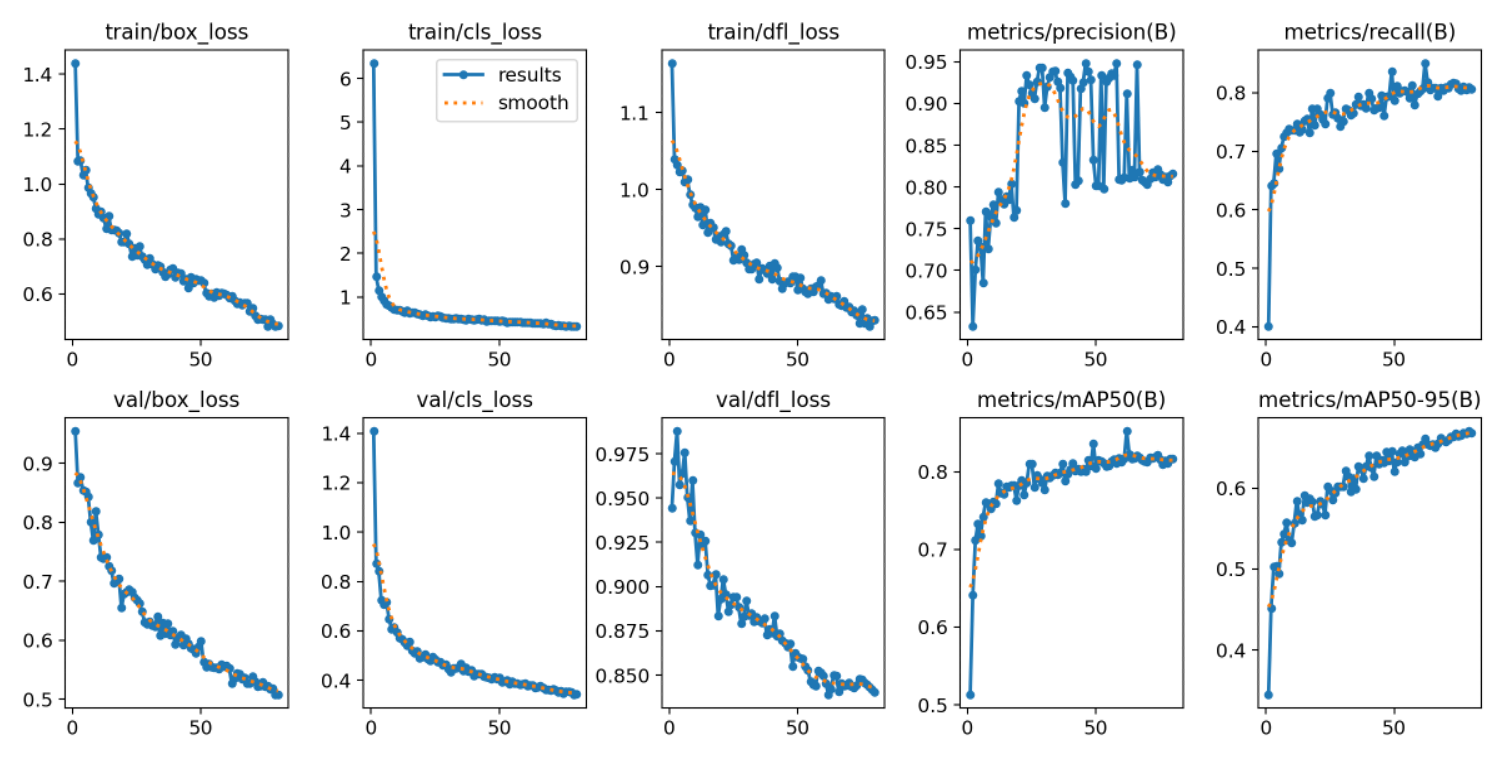
\includegraphics[width=0.85\linewidth]{Images/yolo/YOLO_training.png}
    \caption{YOLOv8 transfer learning convergence showing loss and mean Average Precision (mAP) trends over 80 epochs with the small model.}
    \label{fig:yolo_training_curve}
\end{figure}


%%%%%%%%%%%%%%%%%%%%%%%%%%%%%%%%%%%%%%%%%%%%%%%%%%%%%%%%
\section{GB-CACHE} \label{gbcache}
%\subfile{sections/gbcache}

In parallel with vision-based detection, this research employs the LiDAR-centric method GB-CACHE to represent the class of geometry-driven clustering and segmentation algorithms.
% optimized for sparse maritime environments.
Its name is derived from the methodology it utilizes for object detection: grid-based clustering and concave hull extraction.

The segmentation approach is designed for maritime use, where point cloud data is concentrated on only a few nearby objects.
By ignoring large volumes of unoccupied space, GB-CACHE reduces memory demands and improves processing efficiency.
Its deterministic design and bounded computational complexity make it an optimal choice for real-time operation, and provide a meaningful contrast to the data-intensive, black-box nature of neural-network-based algorithms.
A block diagram of the algorithm is provided in Figure \ref{fig:gbcache_flow}

The algorithm begins by projecting unstructured point cloud data into a spatially organized grid defined in the global fixed frame.
Each point is associated with a primary set of $x$ and $y$ coordinates, and a tertiary $z$ coordinate to preserve vertical geometry.
Segmentation is then performed by clustering adjacent occupied cells in the $x,y$ plane according to a configurable distance parameter.
This dimensionality reduction from three to two spatial dimensions greatly reduces the computational overhead and allows the algorithm to scale linearly with size.

\begin{figure}
    \centering
    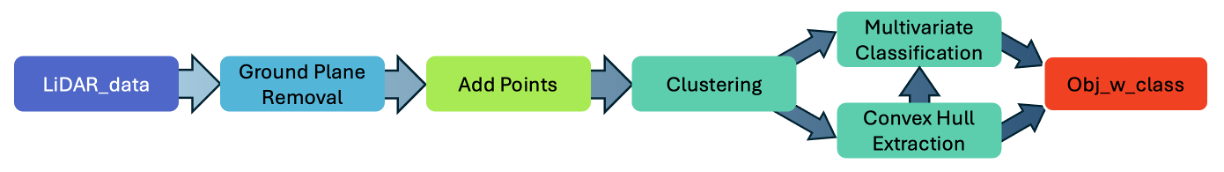
\includegraphics[width=0.95\linewidth]{Images/gbcache/gbcache_flow.png}
    \caption{Block diagram of GB-CACHE process flow.}
    \label{fig:gbcache_flow}
\end{figure}

Each segmented object is then identified by a concave hull formed from the $x$ and $y$ vertices of a perimeter-matched polygon.
Compared to axis-aligned bounding boxes or circular boundary approximations, concave hulls more accurately reflect object geometry without overgeneralizing the object’s spatial extent.

For autonomous navigation, concave hulls offer a balance between fidelity and operational safety.
This is especially relevant in ground-based and maritime environments, where the ability to navigate between closely spaced objects depends on accurately estimating navigable pathways.
Overly conservative bounds may exaggerate the extent of objects as viewed from the vessel.
With precise object boundaries known, they can be inflated to accommodate navigational safety while maintaining an accurate representation of the object's structure.


% \begin{figure}
%     \centering
%     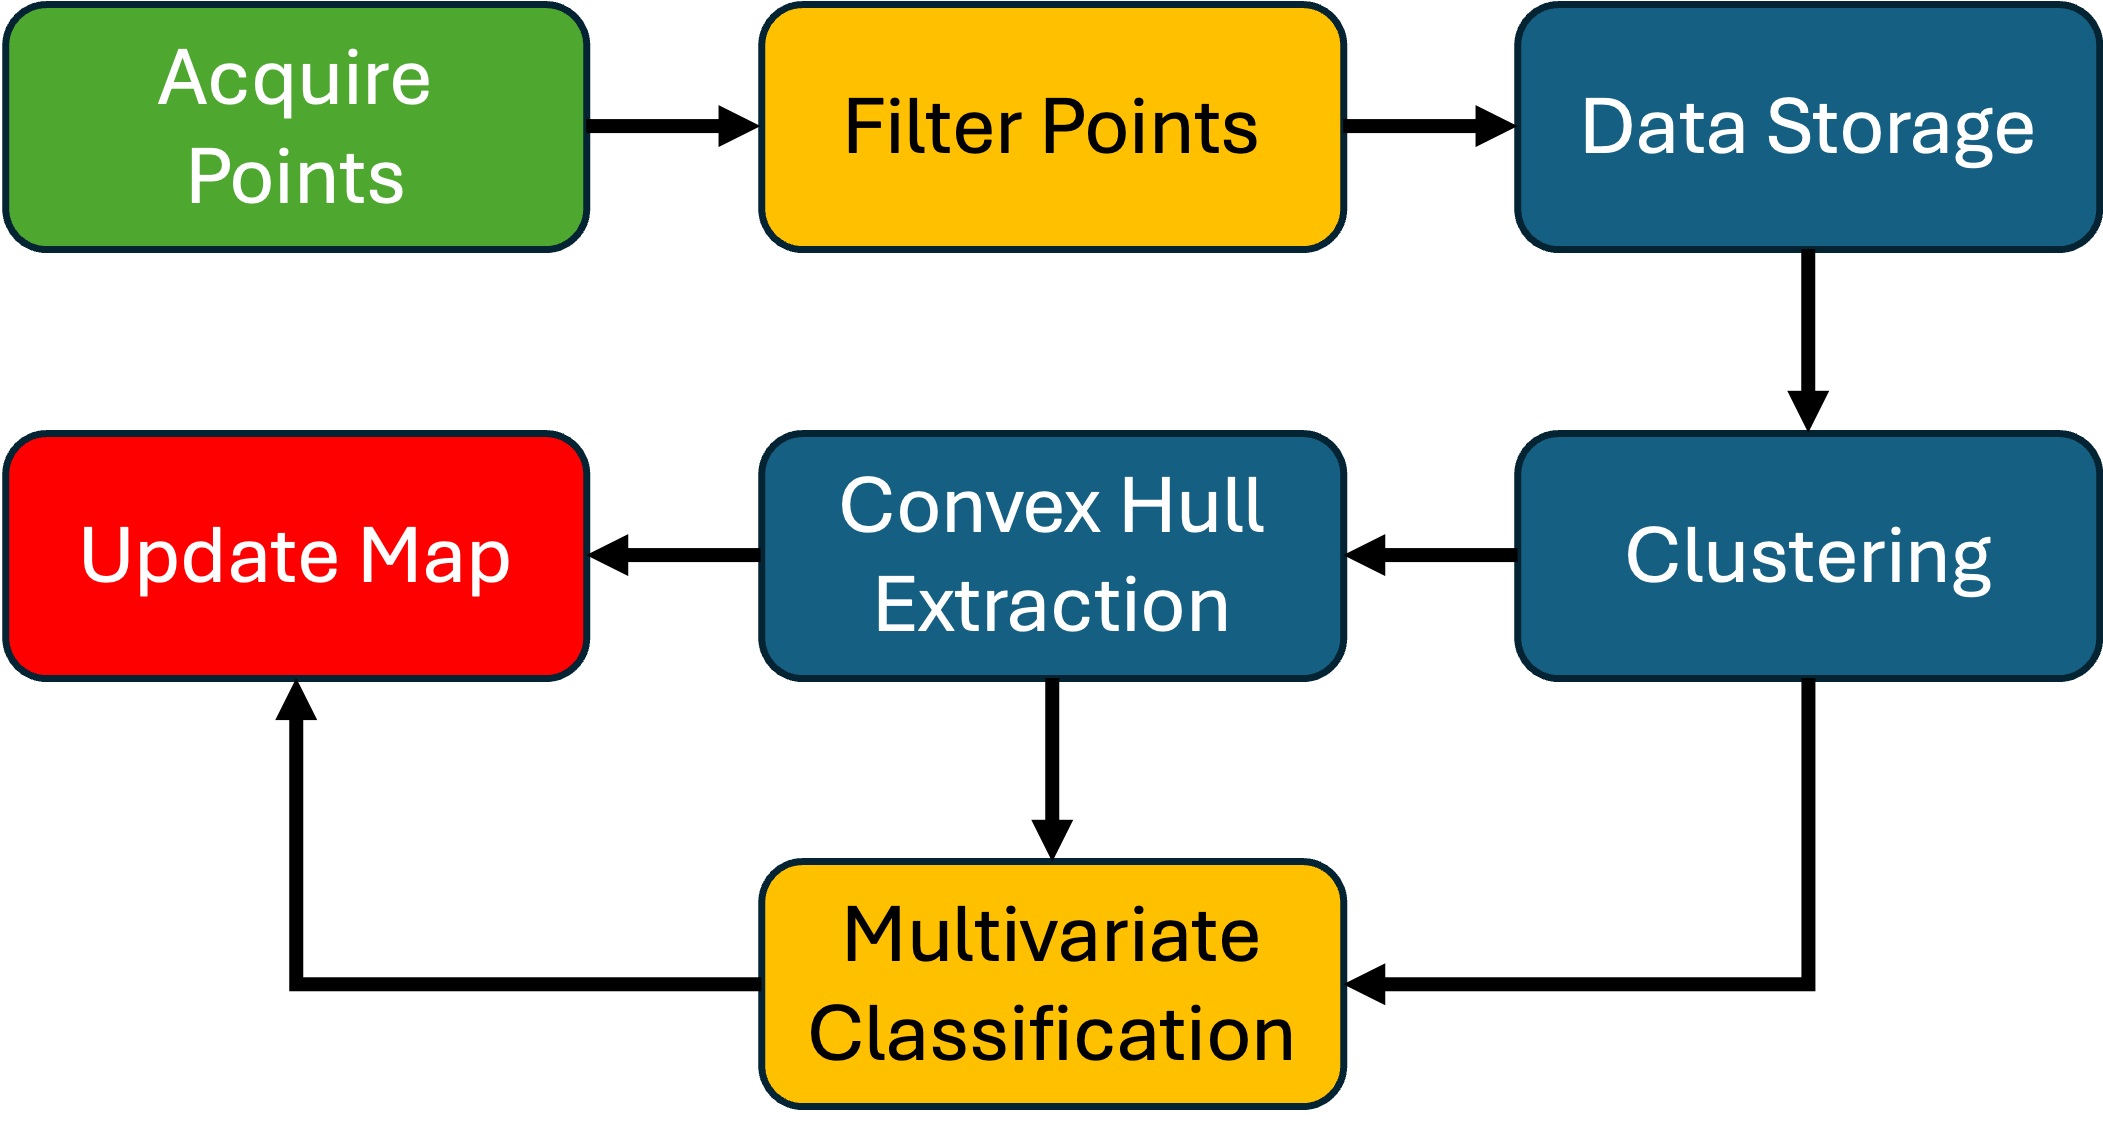
\includegraphics[width=0.95\linewidth]{Images/gbcache_flow.png}
%     \caption{Rectangular bounding boxes placed around maritime objects detected by a re-trained YOLO detection model.}
%     \label{fig:gbcache_flow}
% \end{figure}

% The YOLO Framework
% Describe the principle succinctly:

% YOLOv8 Architecture

% This section should flow from general framework to version-specific improvements:

% Image Resolution and Input Scaling
% Transition to operational detail and experimental consistency:

% Detection Scale and Spatial Sensitivity
% Discuss how feature maps relate to the detection limit:

% Model Constraints and Applicability
% Then note practical limitations and their relevance:

% Implications for Real-Time Fusion
% Conclude the section by connecting to your larger research goal:

% %%%%%%%%%%%%%%%%%%%%%%%%%%%%%%%%%%%%%%%%%%%%%%%%%%%%%%%%%%%%%%%%%%%%
% \subsection{Grid-Based Indexing} \label{sec:grid-based_indexing}

% Reliable object detection from LiDAR data is essential for safe maritime autonomy. To process large three-dimensional point clouds efficiently, this work applies the Grid-Based Clustering and Concave Hull Extraction (GB-CACHE) framework, an existing method developed for real-time segmentation of sparse LiDAR data. The approach enables rapid separation of individual objects while maintaining computational efficiency compatible with embedded vessel hardware.

% GB-CACHE operates by organizing each LiDAR scan into a structured spatial grid, allowing nearby points to be grouped without requiring full pairwise distance comparisons. This grid representation simplifies the process of identifying discrete clusters that correspond to physical objects such as buoys, vessels, or markers. By tuning grid size and connectivity thresholds, the method balances sensitivity to small targets against computational cost. In maritime environments—where LiDAR returns are sparse and concentrated on a few floating objects—the grid structure efficiently isolates relevant regions while ignoring the large volumes of empty space above and below the water surface.

% \begin{figure}
%     \centering
%     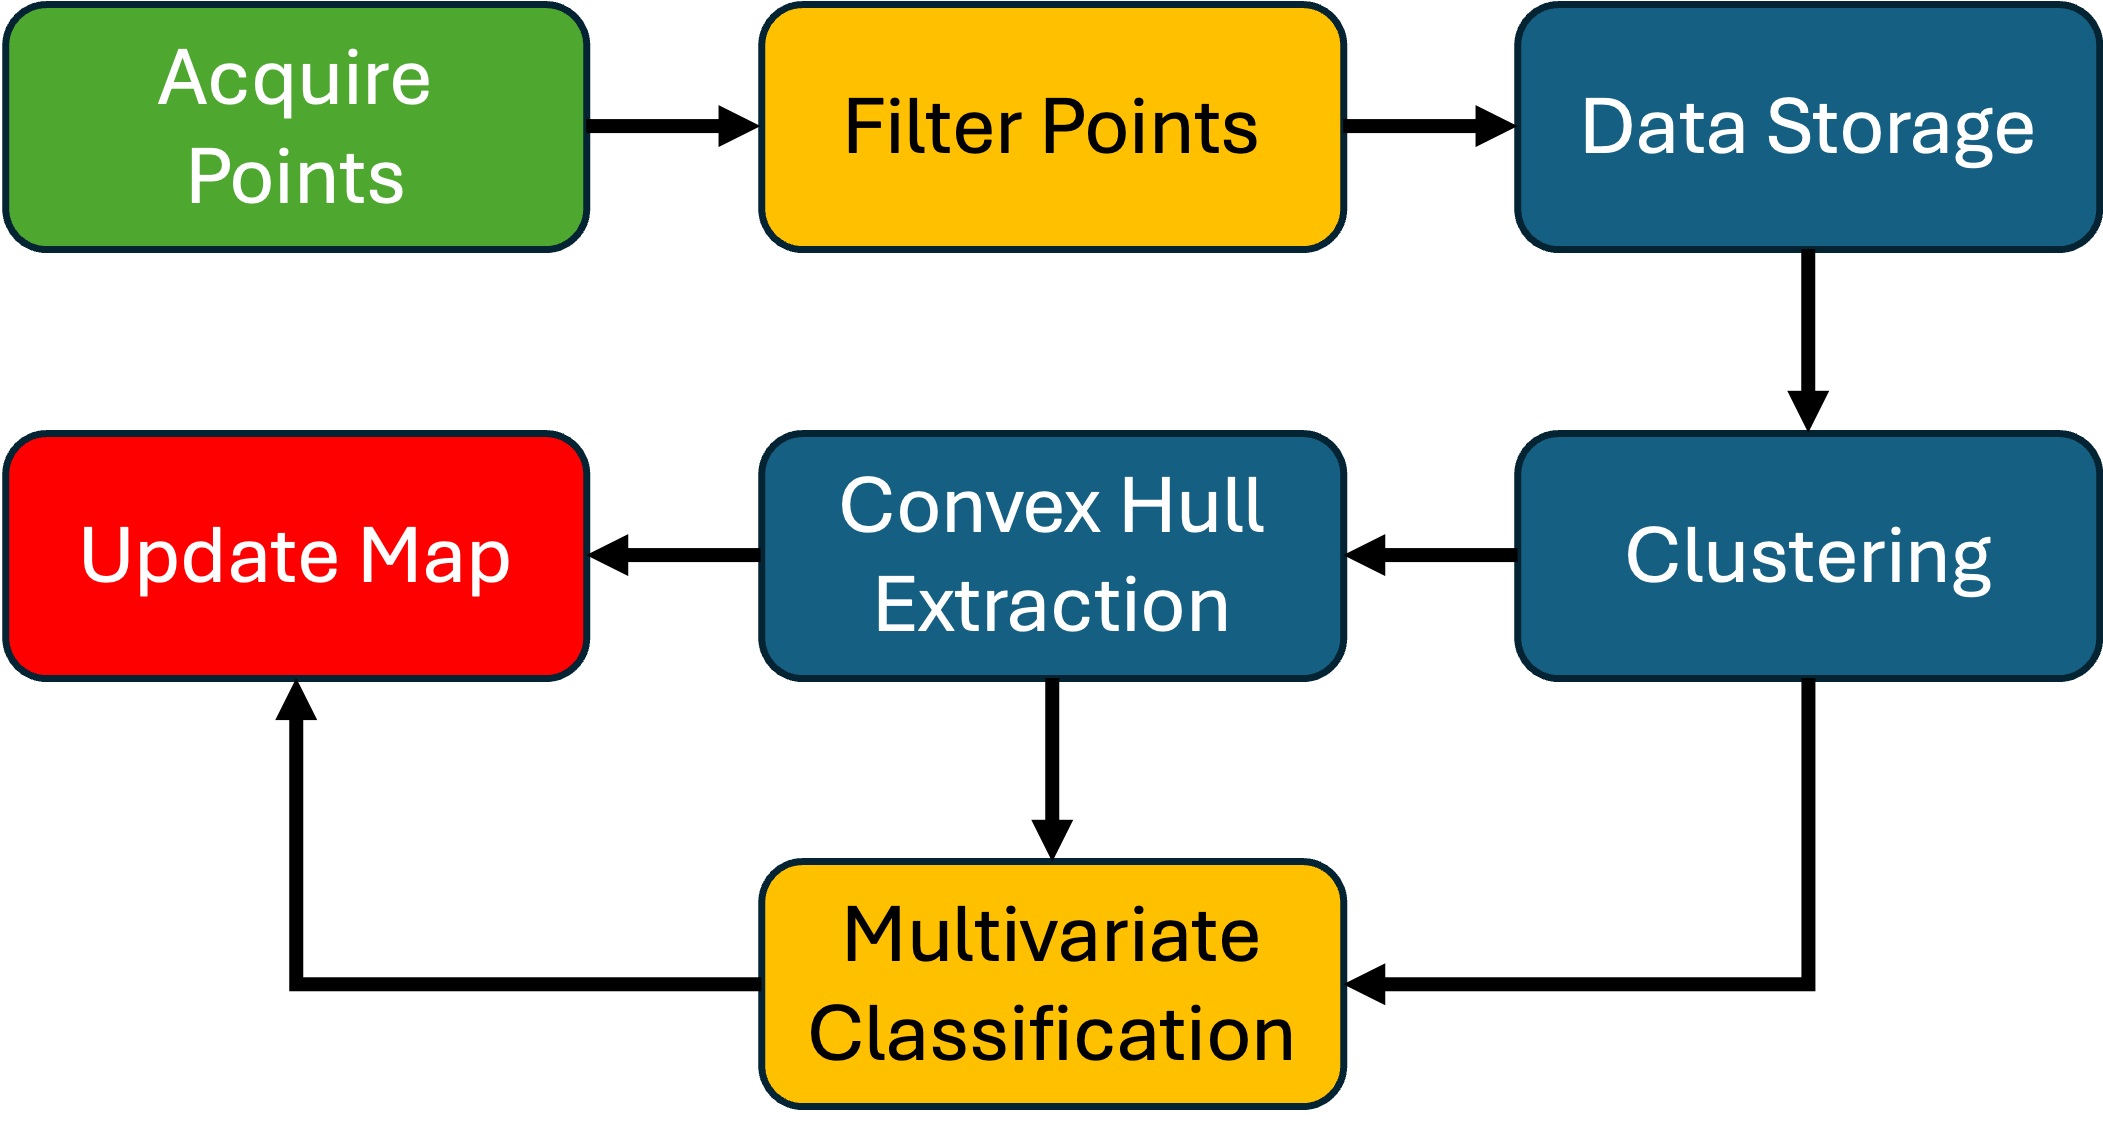
\includegraphics[width=0.5\linewidth]{Images/gbcache_flow.png}
%     \caption{Functional block diagram of the GB-CACHE workflow.}
%     \label{fig:gbcache_flow}
% \end{figure}

% Once potential objects are identified, GB-CACHE extracts geometric boundaries that define their overall shape. Each detected cluster is represented by a concave hull, which conforms closely to the true object outline rather than enclosing it with a simple convex boundary. This representation preserves important geometric details for irregular maritime targets, such as navigation buoys or vessel superstructures, while remaining compact for downstream processing. The resulting shape models form the basis for feature extraction and classification in subsequent stages of the perception pipeline.

% The algorithm’s design emphasizes computational efficiency and predictable timing. Grid-based indexing ensures that processing time scales linearly with the number of points in a scan, allowing consistent real-time performance. Each LiDAR frame is processed independently—populating the grid, segmenting occupied regions, and generating hulls—without maintaining historical state or iterative refinement. This stateless design simplifies implementation and guarantees bounded latency, which is critical for collision-avoidance and control tasks.

% GB-CACHE’s lightweight memory requirements further support real-time operation. Because memory usage scales with grid dimensions rather than total point count, resource consumption remains stable across varying environmental conditions. The method thus provides a practical and computationally efficient means of segmenting maritime LiDAR data into meaningful object candidates, serving as the front-end detection stage for the overall perception system.

% The segmentation stage of \ac{GB-CACHE} produces a structured list of clustered objects, each represented by a polygonal boundary and associated point statistics.
% The multivariate Gaussian classifier (MGC) operates in parallel to this process, classifying each object in the list based on geometric and intensity-derived features computed from its segmented point cloud.
% This architecture separates detection from classification, enabling each to be optimized and evaluated independently while maintaining real-time operation.

% For each detected object, a ten-dimensional feature vector is extracted that captures both spatial geometry and surface reflectivity characteristics.
% The geometric features describe object shape and scale, while the intensity-based features provide cues related to material properties and orientation of reflective surfaces.
% These complementary measurements form a compact yet discriminative representation suitable for statistical classification.
% The selected features are summarized in Table~\ref{tab:features_gbcache}.

% \begin{table}[htbp]
% \centering
% \begin{tabular}{lll}
% \hline
% \multicolumn{3}{c}{GB-CACHE: Object Classification Features}\\
% \hline
% \hline
% \textbf{No.} & \textbf{Feature Type} & \textbf{Description} \\ 
% \hline
% 1 & Maximum Intensity & Peak LiDAR return intensity \\
% 2 & Minimum Intensity & Lowest LiDAR return intensity \\
% 3 & Average Intensity & Mean LiDAR return intensity \\
% 4 & Intensity Standard Deviation & Variation in return intensity \\
% 5 & Maximum Height & Vertical extent of the object \\
% 6 & Filled Cell Count & Number of occupied grid cells \\
% 7 & Polygon Perimeter & Boundary length of concave hull \\
% 8 & Polygon Area & Enclosed area of concave hull \\
% 9 & 2D Minor Axis Length & Shorter principal axis of object shape \\
% 10 & 2D Major Axis Length & Longer principal axis of object shape \\
% \hline
% \end{tabular}
% \caption{Features used for GB-CACHE multivariate classification.}
% \label{tab:gbcache_features}
% \end{table}

% The MGC models the joint probability distribution of these features for each object class under the assumption of Gaussian statistics.
% Each class is represented by its mean vector and covariance matrix, estimated from labeled training data.
% During inference, the classifier computes the likelihood of an observed feature vector under each class model and assigns the class with the highest posterior probability.
% This probabilistic formulation captures correlations among features and yields confidence estimates that can be used downstream in fusion or decision logic.

% Feature-based classification offers several advantages for real-time maritime perception.
% It requires minimal training data, provides interpretability of the decision process, and imposes negligible computational overhead.
% Unlike deep-learning models that operate directly on raw point clouds, the MGC approach allows rapid retraining or adaptation to new object categories without altering the underlying clustering framework.
% This modularity supports continuous improvement and integration within the real-time perception pipeline illustrated in Figure~\ref{fig:gbcache_flow}.

% \begin{figure}[htbp]
%     \centering
%     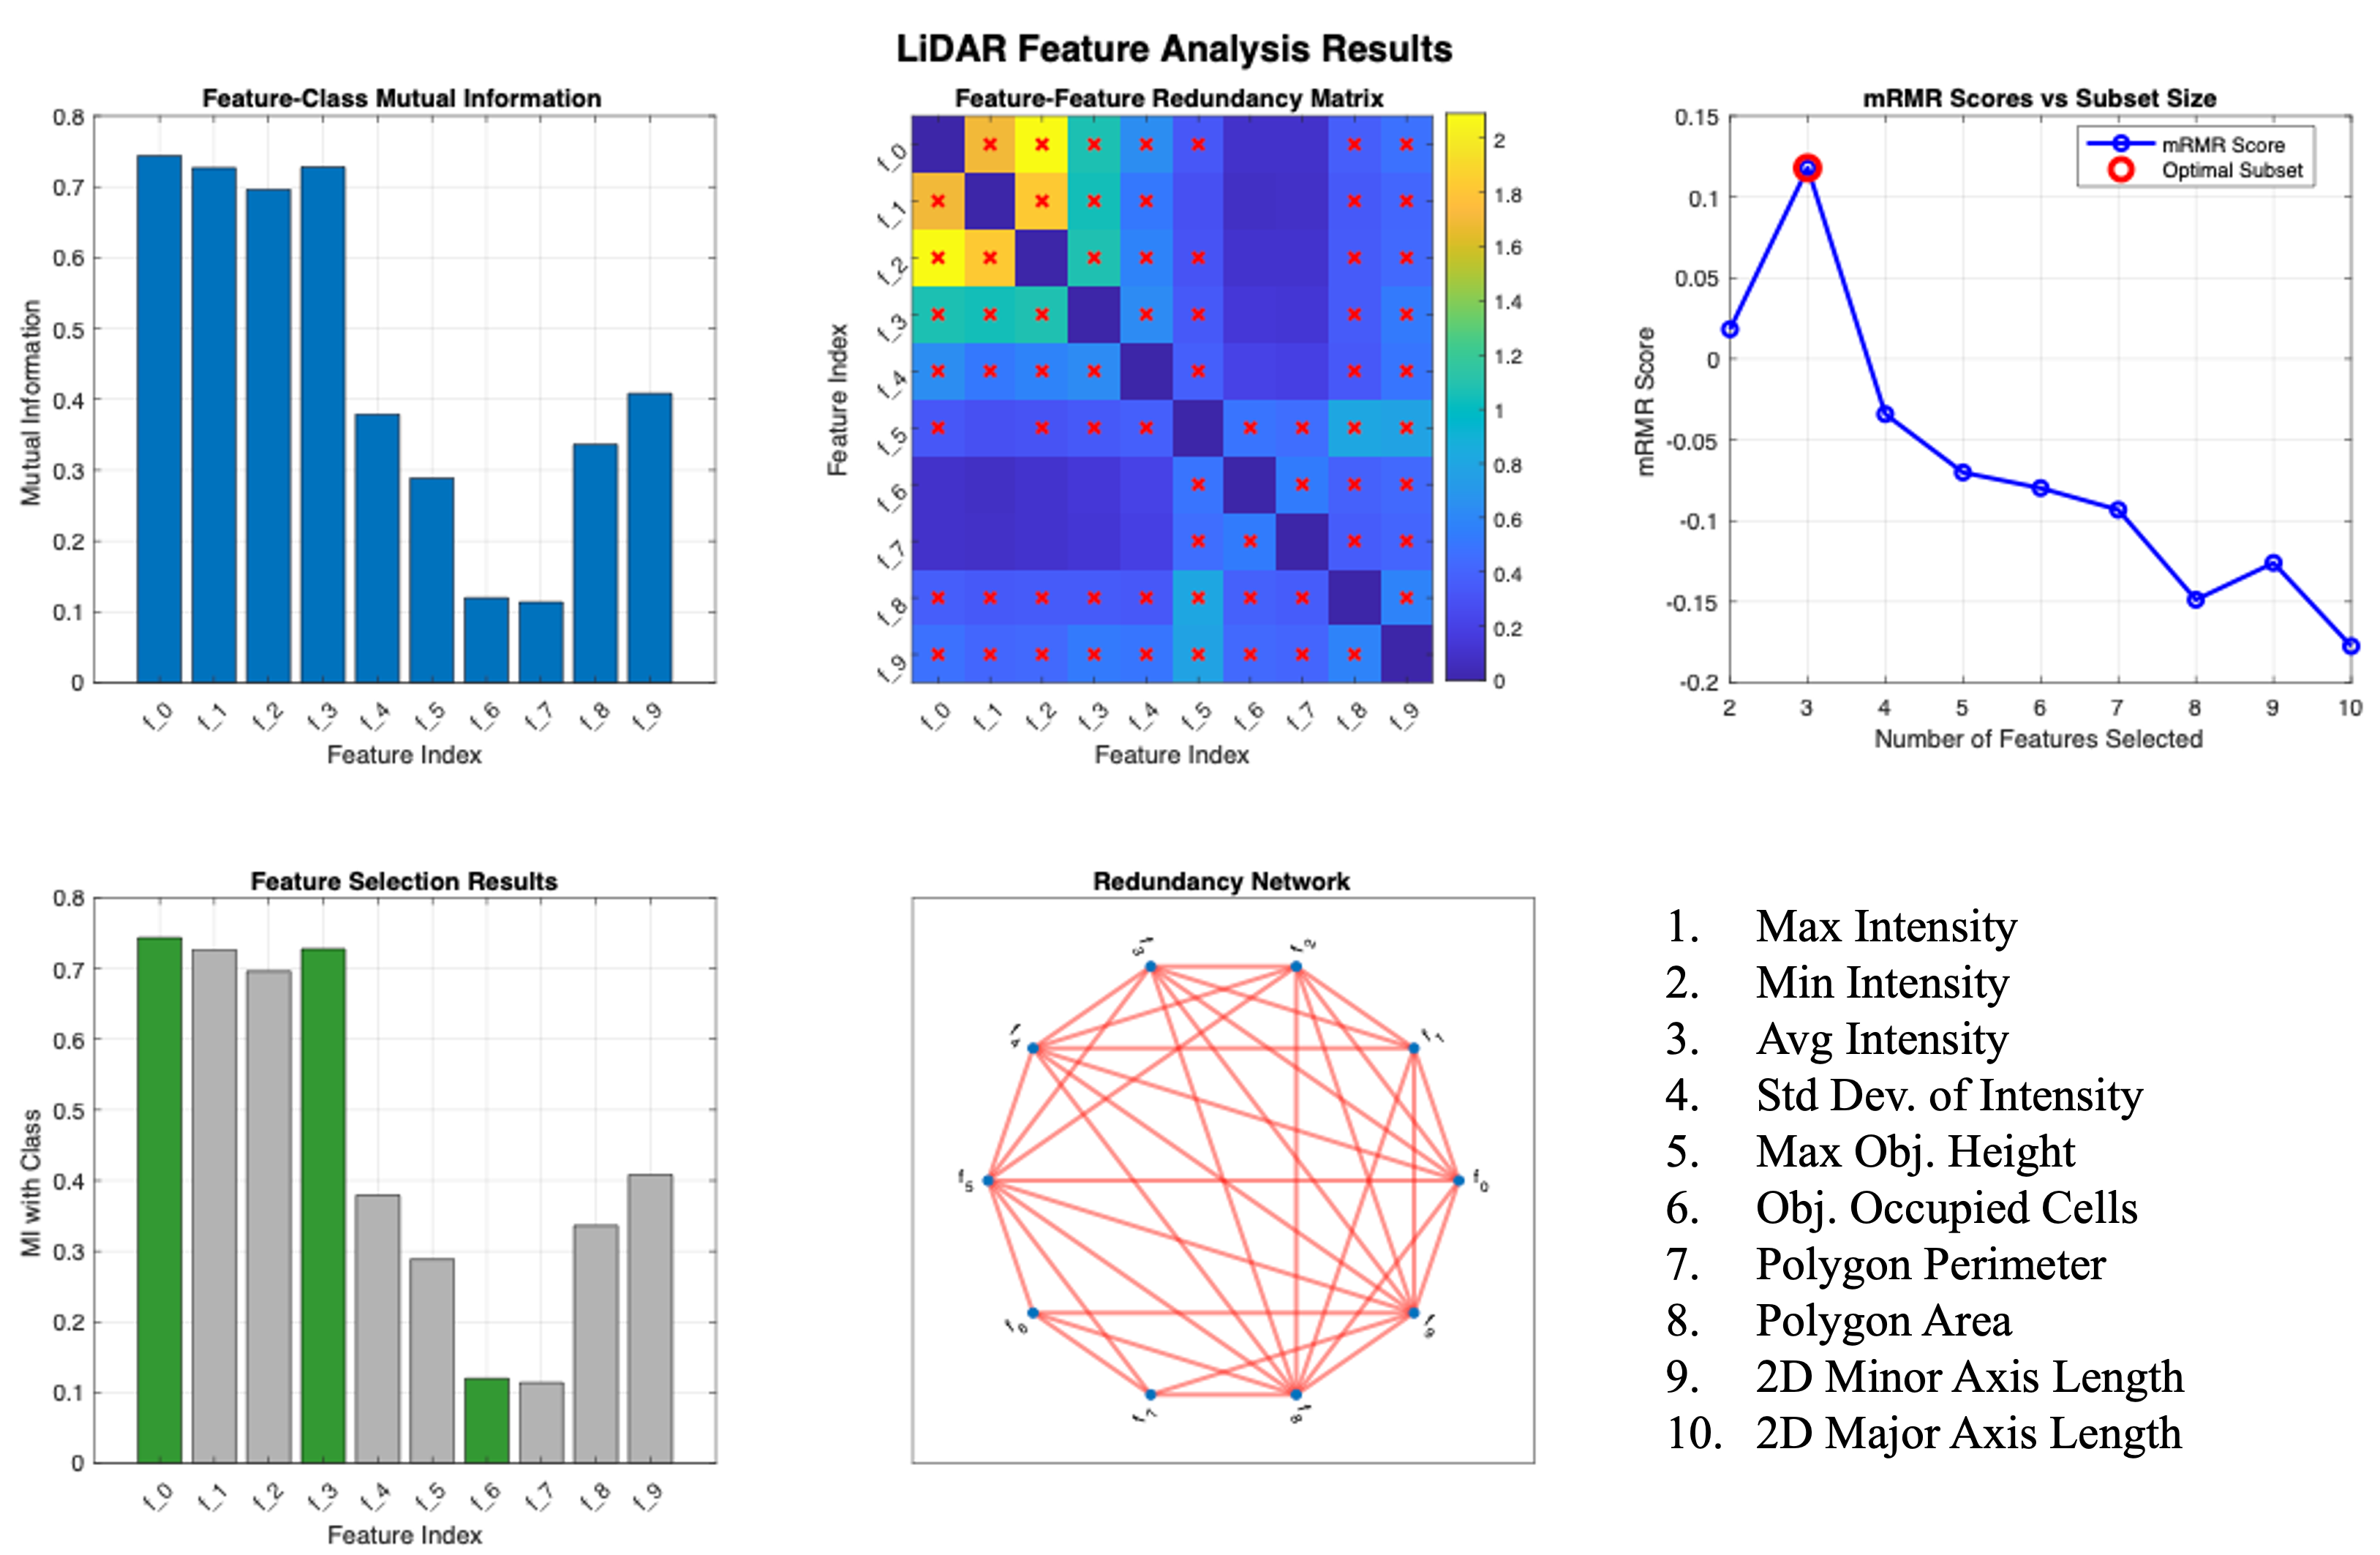
\includegraphics[width=0.95\linewidth]{Images/info_theory_chart_1.png}
%     \caption{Caption}
%     \label{fig:infoTheory_chartsA}
% \end{figure}

% \begin{figure}[htbp]
%     \centering
%     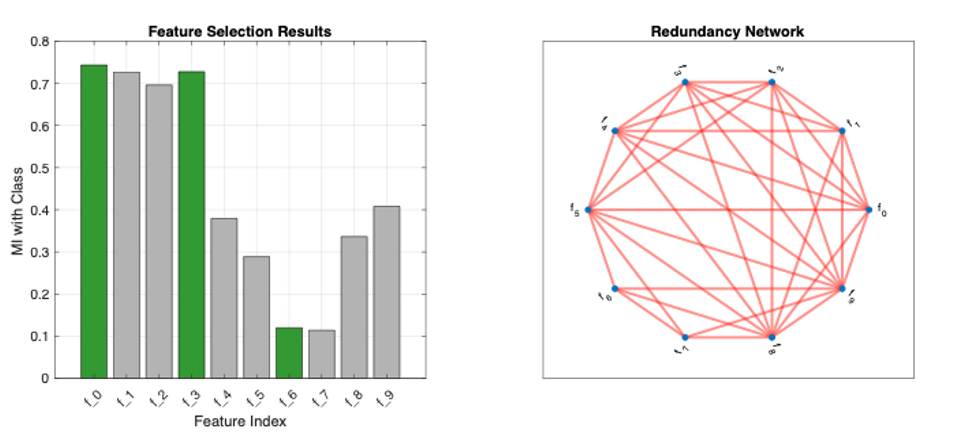
\includegraphics[width=0.8\linewidth]{Images/info_theory_chart_2.png}
%     \caption{Caption}
%     \label{fig:infoTheory_charts}
% \end{figure}

%%%%%%%%%%%%%%%%%%%%%%%%%%%%%%%%%%%%%%%%%%%%%%%%%%%%%%%%
\subsection{GB-CACHE Training Data} \label{training_data_gbcache}

%%%%%%%%%%%%%%%%%%%%%%%%%%%%%%%%%%%%%%%%%%%%%%%%%%%%%%%%
\section{Classification Comparison} \label{sec:classify}
\subsection{Metrics} \label{classify_metrics}
\subsection{Accuracy} \label{classify_accuracy}
\subsection{Timing} \label{classify_timing}


%%%%%%%%%%%%%%%%%%%%%%%%%%%%%%%%%%%%%%%%%%%%%%%%%%%%%%%%
\subsection{YOLO Performance} \label{performance_yolo}




The fine-tuned YOLOv8-s model achieved the best balance of accuracy and speed for maritime operations.
Model evaluation was performed using a holdout dataset collected under variable illumination and sea states.
Performance metrics include mean Average Precision (mAP@50), precision-recall curves, and confusion matrices for key object classes such as vessels, buoys, and docks.

\begin{figure}[htbp]
    \centering
    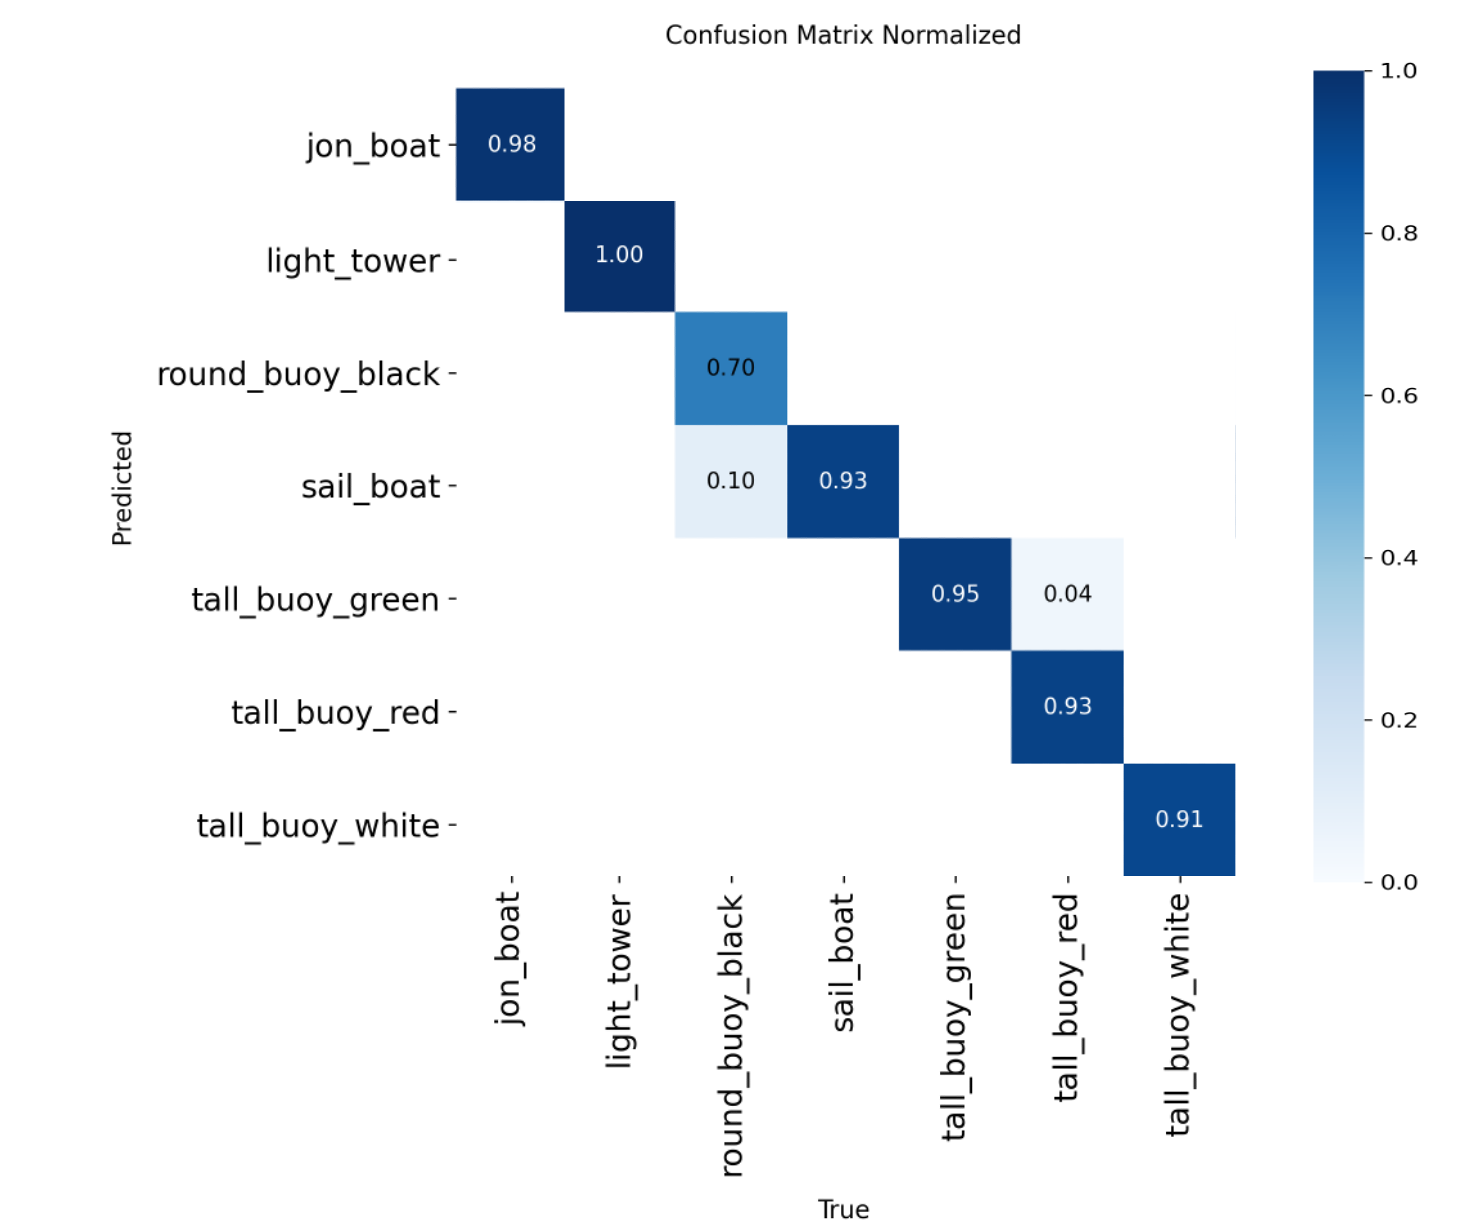
\includegraphics[width=0.8\linewidth]{Images/yolo/YOLO_training_results.png}
    \caption{Confusion matrix for YOLOv8-s model evaluated on the test dataset.}
    \label{fig:yolo_confusion_matrix}
\end{figure}

% \begin{figure}[htbp]
%     \centering
%     \includegraphics[width=0.8\linewidth]{Images/yolo_pr_curve.png}
%     \caption{Precision–recall curve for primary object classes.}
%     \label{fig:yolo_pr_curve}
% \end{figure}

Results indicate consistent detection performance across lighting conditions with minimal false positives on horizon clutter.
Retraining improved small-object detection by approximately X\% compared to baseline COCO-trained weights, confirming the benefit of domain adaptation for maritime imagery.

The fine-tuned YOLOv8 network serves as the visual baseline for comparison with LiDAR-based object detection methods presented in Section~\ref{gbcache}.
By isolating timing metrics for each processing stage, the performance comparison remains hardware-agnostic.
This approach emphasizes algorithmic latency, rather than total frame rate, as the primary metric for evaluating real-time feasibility in multi-sensor fusion.

%%%%%%%%%%%%%%%%%%%%%%%%%%%%%%%%%%%%%%%%%%%%%%%%%%%%%%%%
\subsection{GB-CACHE Performance} \label{performance_gbcache}

A mutual information (MI) framework was used to quantify the statistical dependence between each LiDAR-derived feature and the corresponding object class label used in the multivariate Gaussian classifier. 
The objective of this analysis was to determine which features contributed the greatest amount of information for class discrimination, as well as to identify any redundant or weakly informative features.

Each feature vector consisted of ten geometric and intensity-based descriptors extracted from clustered LiDAR objects, including metrics such as concave-hull perimeter, projected area, principal axis lengths, circularity, and statistical measures of return intensity. 
The feature set was standardized to zero mean and unit variance prior to analysis to prevent scale-dependent bias in the estimator.

Mutual information values were computed between each individual feature $x_i$ and the discrete class label $y$ using
\[
I(x_i; y) = \sum_{x_i,y} p(x_i, y) \log \frac{p(x_i, y)}{p(x_i) p(y)},
\]
where $p(x_i, y)$ is the joint probability distribution estimated from the dataset.
Continuous-valued features were discretized into an adaptive number of bins based on quantiles to balance estimator bias and variance.
The resulting $I(x_i; y)$ values represent the reduction in uncertainty of the class label given knowledge of each feature.

Pairwise feature–feature mutual information values $I(x_i; x_j)$ were also computed to evaluate redundancy among features and to support subsequent feature selection using the minimum redundancy–maximum relevance (mRMR) criterion.

Features related to object geometry, such as perimeter and projected area, exhibited the highest mutual information with class labels, indicating that spatial extent and shape are the most discriminative descriptors within the dataset. 
Intensity-based and statistical features showed moderate information gain, while derived ratios and higher-order shape factors contributed marginally.

Pairwise feature–feature analysis revealed moderate redundancy between perimeter and area, as expected from their geometric relationship, but limited redundancy across the remaining features. 
The mRMR ranking procedure identified [placeholder feature names] as the most informative subset for classification, providing a compact feature set with minimal information overlap.

Overall, the mutual information results confirm that geometric descriptors carry the dominant class-discriminative content in the LiDAR feature set, while statistical and textural measures provide supplementary but nonessential information. 
These findings guided the dimensionality reduction and feature selection strategies adopted for the multivariate Gaussian classifier.



% \subsection{Computational Efficiency} \label{sec:gbcache_efficiency}

The algorithmic design of \ac{GB-CACHE} prioritizes computational efficiency to enable real-time processing on autonomous surface vessel hardware with limited computing resources.
Grid-based spatial indexing reduces clustering complexity from quadratic to linear in the number of points, while the regular grid structure enables vectorized operations and cache-efficient memory access patterns.
These optimizations prove essential for maintaining detection frame rates sufficient for autonomous navigation, where delayed perception degrades collision avoidance performance.

The GB-CACHE processing pipeline operates incrementally on each \ac{LiDAR} scan, maintaining no temporal history and requiring no iterative refinement.
This design guarantees bounded worst-case execution time, critical properties for safety-critical autonomous systems.
Each scan undergoes independent processing: grid population, clustering, hull extraction, and feature calculation, producing object detections with consistent latency.

Memory requirements scale with grid dimensions rather than point count, providing predictable resource consumption independent of scene complexity.
The grid representation compresses sparse maritime point clouds into compact occupancy structures, reducing memory bandwidth requirements compared to maintaining full point coordinates.
This compression proves particularly advantageous for maritime environments where objects occupy a small fraction of the sensor's field of view.

\begin{figure}
    \centering
    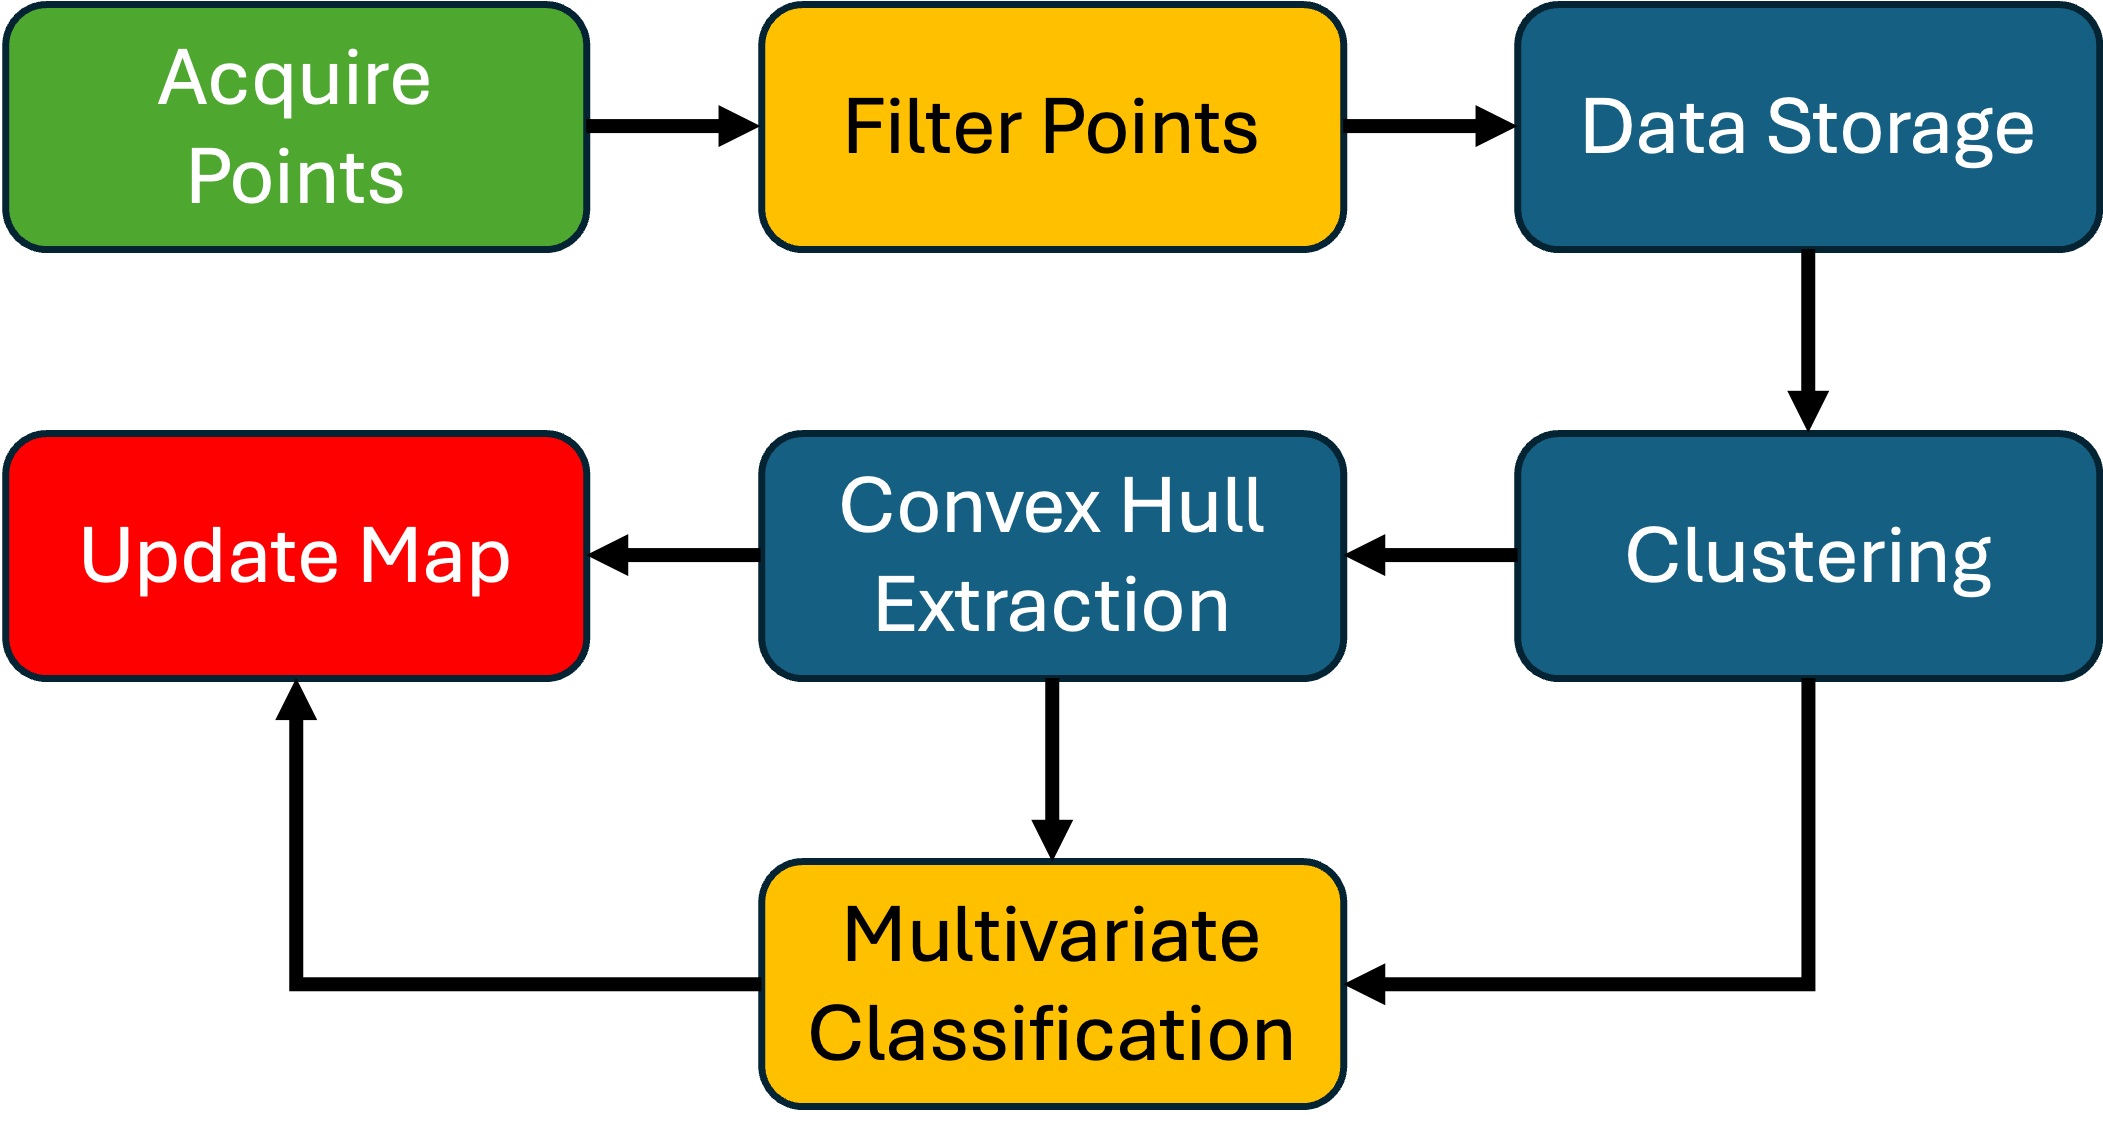
\includegraphics[width=0.95\linewidth]{Images/gbcache_flow.png}
    \caption{The three main portions of the GB-CACHE process which were examined for performance}
    \label{fig:gbcache_flow_analysis}
\end{figure}

Performance analysis of the \ac{GB-CACHE} implementation on the Minion platform demonstrates exceptional computational efficiency compatible with real-time autonomous navigation requirements.
The spatial filtering and point addition operations execute with sub-millisecond latency, consuming negligible fractions of available processing time at sensor frame rates.
The map update operation, while more computationally intensive, exhibits strong linear correlation with object geometric complexity, specifically polygon perimeter and surface area.
This predictable scaling behavior enables reliable worst-case execution time estimation for safety-critical autonomous systems.
Hardware resource utilization remains minimal during typical operation, with both processor and memory consumption well below capacity thresholds, providing substantial computational headroom for concurrent navigation and control processes.
Detailed performance characterization across diverse maritime object encounters validates the algorithm's suitability for sustained real-time operation under operational constraints.

% \subsection{GB-CACHE Execution Performance}
%%%% GPT analysis of results
To evaluate computational performance, execution times were recorded for each GB-CACHE subroutine across all processed ROS bag datasets. 
Each subroutine timing corresponded to a complete call of its respective function, and timestamps were generated on a single synchronized host computer to ensure consistent temporal reference.

Three primary subroutines within the GB-CACHE processing loop were instrumented for timing, as illustrated in Figure~\ref{fig:gbcache_flow_analysis}. 
These correspond to the sequential stages that handle LiDAR data input, spatial filtering, and map updating during each processing cycle. 
Each subroutine represents a distinct computational task within the overall workflow, encompassing the removal of irrelevant ground-plane returns, the insertion of new point data into the cache, and the segmentation and classification of clustered features used for object detection.

Each event was logged during runtime and later analyzed in MATLAB to determine average duration, execution frequency, and utilization of available processing time. 
Outliers above the 99.5th or 99.9th percentile were discarded to remove statistical noise caused by transient load conditions.

% \subsubsection*{Results}
\begin{table}[htbp]
\centering
\begin{tabular}{lccccc}
\hline
Subroutine & Samples & Avg Duration (ms) & Allotted Time (ms) & \% of Allotted Time\\
\hline
Filter Points & 1,701,153 & 0.009 &  3.33 & 0.26 \% \\
Add Points & 1,701,153 & 0.140 &  3.33 & 4.21 \% \\
Update Map & 45,746 & 8.002 & 200 & 4.00 \% \\
\hline
\end{tabular}
\caption{Average execution time and percentage of allotted processing time for each GB-CACHE subroutine.}
\label{tbl:gbcache_subroutine_results}
\end{table}

The results show that all GB-CACHE operations complete well within their real-time deadlines. 
The \textit{Filter Points} and \textit{Add Points} stages execute on the order of microseconds to sub-milliseconds, together consuming less than five percent of their available 3.33~ms cycle time. 
The \textit{Update Map} stage, which performs segmentation and classification, operates at 5~Hz and occupies approximately four percent of its 200~ms time window.

% \subsubsection*{Interpretation}
The findings indicate that GB-CACHE’s computational performance is dominated by the segmentation and classification phase, yet remains well below the latency threshold required for real-time operation. 
The lightweight filtering and data-insertion routines contribute negligibly to total cycle time. 
Polynomial regression and correlation analysis further confirmed that \textit{Update Map} duration scales with scene complexity---specifically, with total feature perimeter and area---while \textit{Filter Points} and \textit{Add Points} remain largely invariant.

Overall, the analysis demonstrates that GB-CACHE can sustain real-time performance on the tested hardware with significant computational margin for additional perception or control tasks.

\begin{figure}[htbp]
\centering
\makebox[\textwidth][c]{
    \begin{subfigure}[t]{0.44\textwidth}
        \centering
        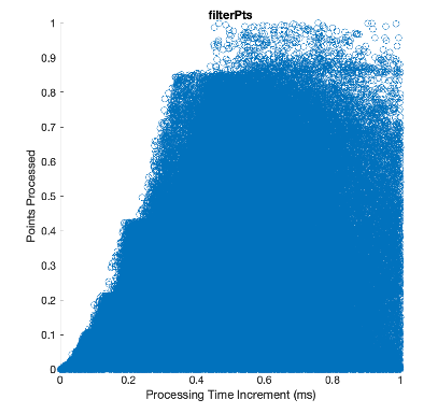
\includegraphics[width=\textwidth]{Images/gbcache/filter_points_scatter.png}
        \caption{Scatter plot of duration of \texttt{filter\_points} against number of LiDAR points}
        \label{fig:gbcache_filter_points_scatter}
    \end{subfigure}
    \hspace{2em} % horizontal spacing between them
    \begin{subfigure}[t]{0.44\textwidth}
        \centering
        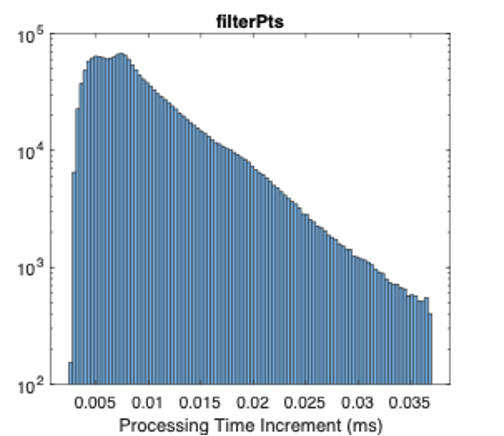
\includegraphics[width=\textwidth]{Images/gbcache/filter_points_hist.png}
        \caption{Histogram of duration of \texttt{filter\_points} against number of LiDAR points}
        \label{fig:gbcache_filter_points_hist}
    \end{subfigure}
}
\caption{Scatter (a) and histogram (b) plots of \texttt{filter\_points} process plotted against number of LiDAR points}
\label{fig:gbcache_filter_points}
\end{figure}

\begin{figure}[htbp]
\centering
\makebox[\textwidth][c]{
    \begin{subfigure}[t]{0.44\textwidth}
        \centering
        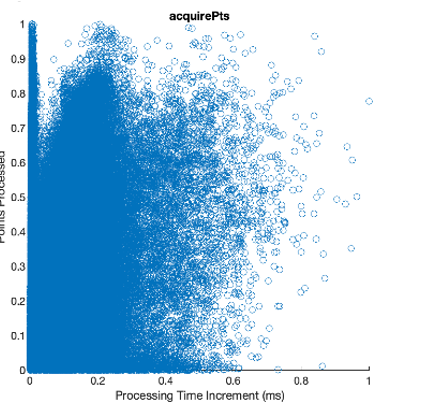
\includegraphics[width=\textwidth]{Images/gbcache/Add_points_scatter.png}
        \caption{Scatter plot of duration of \texttt{add\_points} against number of LiDAR points}
        \label{fig:gbcache_add_points_scatter}
    \end{subfigure}
    \hspace{2em} % horizontal spacing between them
    \begin{subfigure}[t]{0.44\textwidth}
        \centering
        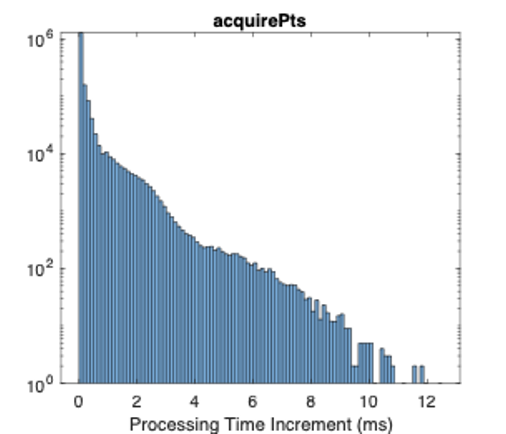
\includegraphics[width=\textwidth]{Images/gbcache/Add_points_hist.png}
        \caption{Histogram of duration of \texttt{add\_points} against number of LiDAR points}
        \label{fig:gbcache_add_points_hist}
    \end{subfigure}
}
\caption{Scatter (a) and histogram (b) plots of \texttt{add\_points} process plotted against number of LiDAR points}
\label{fig:gbcache_add_points}
\end{figure}

\begin{figure}[htbp]
    \centering
    % Subfigure (a)
    \begin{subfigure}[b]{0.44\linewidth}
        \centering
        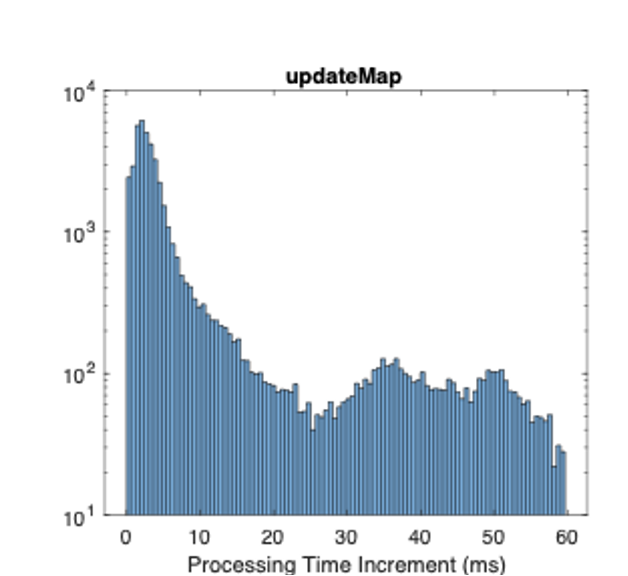
\includegraphics[width=\linewidth]{Images/gbcache/Update_Map_hist.png}
        \caption{Histogram of duration of \texttt{map\_update} against number of LiDAR points}
        \label{fig:gbcache_update_map_hist}
    \end{subfigure}
    \vspace{1em} % vertical spacing between subfigures
    % Subfigure (b)
    \begin{subfigure}[b]{0.8\linewidth}
        \centering
        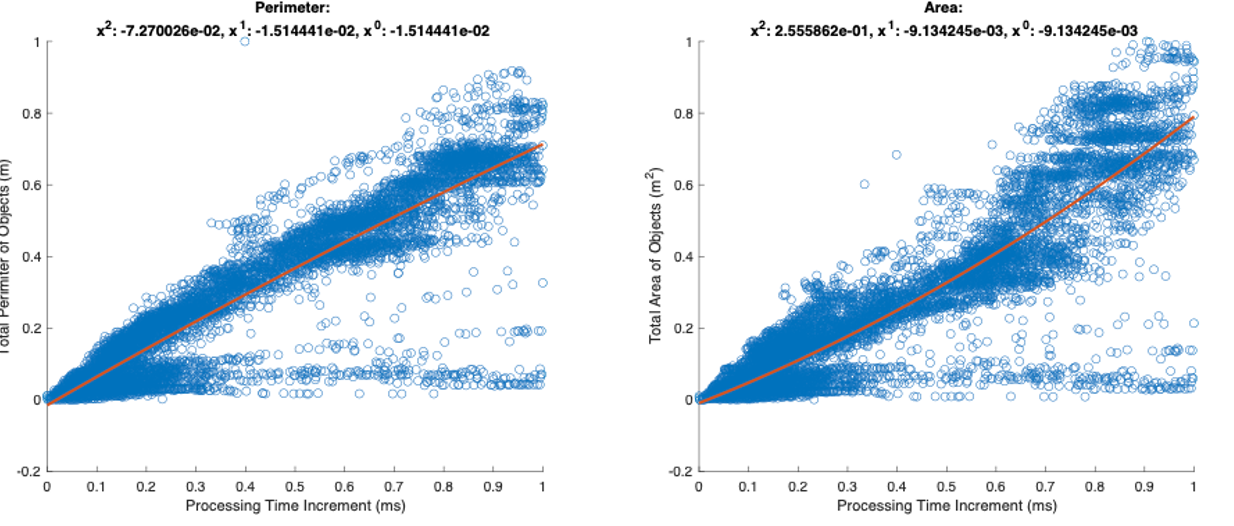
\includegraphics[width=\linewidth]{Images/gbcache/Update_Map_scatter.png}
        \caption{Two scatter plot of duration of \texttt{map\_update} against average perimeter length of polygon (left), and against average area of polygon (right). The line of best-fit is shown in red for each, with associated polynomial values of: $x^2 = -0.0727, x^1 = -0.0151, x^0 = -0.0151$ (left) and $x^2 = 0.2556, x^1 = -0.00913, x^0 = -0.00913$ (right) }
        \label{fig:gbcache_update_map_scatter}
    \end{subfigure}

    \caption{Histogram (a) and scatter (b) plots of \texttt{map\_update} process plotted against number of LiDAR points}
    \label{fig:gbcache_update_map}
\end{figure}

%%%%%%%%%%%%%%%%%%%%%%%%%%%%%%%%%%%%%%%%%%%%%%%%%%%%%%%%
\subsection{Feature Relevance} \label{features}

\subsubsection{YOLO Features} \label{features_yolo}

\subsubsection{GB-CACHE Features} \label{features_gbcache}

GB-CACHE employs a \acl{MGC} to specify what class of object it has identified. 
Much like other classification methods, it utilizes a list of detected features to distinguish one class from another.
Each of the ten features it observes is provided with a brief description in Table \ref{tab:gbcache_features}.
The magnitude of an object's observed individual features may change based on distance to the object or viewing angle, but their relative values still provide valuable information.

\begin{table}[htbp]
\centering
\begin{tabular}{lll}
\hline
\multicolumn{3}{c}{GB-CACHE: Object Classification Features}\\
\hline
\hline
\textbf{No.} & \textbf{Feature Type} & \textbf{Description} \\ 
\hline
1 & Intensity (Max) & Peak LiDAR return intensity \\
2 & Intensity (Min) & Lowest LiDAR return intensity \\
3 & Intensity (Avg) & Mean LiDAR return intensity \\
4 & Intensity (Std. Deviation) & Variation in return intensity \\
5 & Height (Max) & Vertical extent of the object \\
6 & Filled Cell Count & Number of occupied grid cells \\
7 & Polygon Perimeter & Length of 2D concave hull boundary \\
8 & Polygon Area & Area of enclosed 2D concave hull \\
9 & Major Axis Length & Longer principal axis of object polygon \\
10 & Minor Axis Length & Shorter principal axis of object polygon \\
\hline
\end{tabular}
\caption{Features used for GB-CACHE multivariate classification.}
\label{tab:gbcache_features}
\end{table}

In \ac{MGC}, the values of these features are assumed to follow Gaussian distributions within each class.
By modeling the joint distribution of all ten features at once (a multivariate Gaussian), the classifier can compute a \acl{PDF} for each object class.
This enables the classifier to assign the most probable class label to the object based on the vector of all ten features, even as the individual values may fluctuate.

% \subsection{Mutual Information Analysis of Features} \label{sec:gbcache_MI_features}

While the ten-feature set provides comprehensive object characterization, not all features contribute equally to classification performance, and some features exhibit redundancy through correlation.
I applied information-theoretic feature selection methodology to identify the optimal feature subset that maximizes classification accuracy while minimizing computational burden and correlation-induced instability.

The minimum Redundancy Maximum Relevance (mRMR) criterion provides a principled framework for feature selection by simultaneously considering two competing objectives: maximizing the mutual information between selected features and class labels (relevance) while minimizing the mutual information among selected features themselves (redundancy).
Mutual information quantifies the reduction in uncertainty about one variable given knowledge of another, providing a model-agnostic measure of statistical dependence applicable to both linear and nonlinear relationships.

Analysis of feature-class mutual information reveals varying discriminative power across the ten features, with intensity-based and geometric features exhibiting complementary strengths for different object classes.
Pairwise feature redundancy analysis identifies multiple correlated feature pairs that provide overlapping information, suggesting opportunities for dimensionality reduction without classification performance degradation.
The mRMR optimization procedure balances these considerations, progressively selecting features that contribute novel discriminative information while avoiding redundant measurements.

Information-theoretic analysis identified an optimal feature subset substantially smaller than the complete ten-feature set, demonstrating that effective maritime object classification can be achieved with reduced feature dimensionality.
This finding has practical implications for computational efficiency, as feature extraction and Gaussian density evaluation scale with feature dimensionality.
The reduced feature set maintains robust classification performance while decreasing processing requirements and reducing the risk of overfitting when training data is limited.

The classifier requires training data comprising labeled examples of each object class with corresponding feature vectors.
Training involves computing maximum likelihood estimates of Gaussian distribution parameters for each class, specifically the mean vector and covariance matrix that characterize the feature space distribution.
These parameters fully specify the class models, enabling rapid inference through simple multivariate Gaussian density evaluation without iterative optimization or complex neural network forward passes.

Classification performance depends critically on the separability of object classes in the chosen feature space and the validity of the Gaussian distribution assumption.
When classes exhibit significant overlap in feature space or when feature distributions deviate substantially from Gaussian, classification accuracy degrades.
However, for maritime objects with distinct geometric profiles and size ranges, the feature-based Gaussian approach provides robust classification with minimal training requirements.

%%%%%%%%%%%%%%%%%%%%%%%%%%%%%%%%%%%%%%%%%%%%%%%%%%%%%%%%
\section{Detection Results} \label{detect_results}

\subsection{Metrics} \label{detect_metrics}
\subsection{YOLO} \label{detect_yolo}
\subsection{GB-CACHE} \label{detect_gbcache}
% \subsection{Image Frame Bias} \label{detect_imgFrame_bias}

%%%%%%%%%%%%%%%%%%%%%%%%%%%%%%%%%%%%%%%%%%%%%%%%%%%%%%%%
\section{Late Fusion} \label{fusion}
\subsection{Method} \label{fusion_method}
\subsection{Justification} \label{fusion_justificaiton}





\chapter{Conclusions}
% This chapter will synthesize findings from all three research objectives:
% - Summary of comparative performance results between LiDAR and vision systems
% - Calibration and synchronization framework effectiveness
% - Real-time processing capability validation
% - Implications for ASV perception system design
% - Contribution to maritime autonomous systems knowledge

% \section{Research Objective Achievement Summary}
% \subfile{}
% Placeholder for objective completion summary

% \section{Performance Comparison Findings}
% \subfile{}
% Placeholder for key comparative analysis conclusions

% \section{Implications for ASV System Design}
% \subfile{}
% Placeholder for practical design guidance conclusions


\chapter{Recommendations and Future Work} \label{chap:recommendations}
% \subfile{sections/real_time_obj_det}
% a brief introduction to the chapter 

% \section{Recommendations} \label{sec:recommendations}
% \subfile{)

\section{Future Work} \label{futurework}

% This dual-system configuration facilitated the transition of Minion's software during the period of this research.
% \ac{ROS} 1 was the operational framework for all research and data collected in this study, however, \ac{ROS} 1 has entered end-of-life for active development.
% Consequently, Minion’s software architecture was gradually migrated to \ac{ROS} 2, which introduces substantial improvements in real-time performance, memory management, and inter-process communication.
% In contrast to ROS 1’s reliance on a centralized message broker, ROS 2 employs a Data Distribution Service-based communication layer that reduces latency and memory overhead through zero-copy data handling and improved resource allocation.
% Maintaining one system on ROS 1 while transitioning the other to ROS 2 allowed incremental software migration without interrupting field operations—laying the groundwork for future runtime performance improvements anticipated in Section~\ref{futurework}.


% \section{ASV Perception System Design Recommendations}
% \subfile{}
% Placeholder for design guidance recommendations

% \section{Future Research Directions}
% \subfile{}
% Placeholder for future work recommendations

% \section{Technology Transfer Opportunities}
% \subfile{}
% Placeholder for practical application recommendations




% \printbibliography
% \bibliographystyle{plainnat} - Most recent
\bibliographystyle{IEEEtranN} % natbib-compatible numeric IEEE style
% \bibliography{References}
\bibliography{Dissertation,extra_cite}

\backmatter


\chapter{Image Transform} \label{img_tform}
\subfile{sections/img_tform}

\chapter{Video Encoding and Timestamp Pipeline} \label{append_video_pipeline}

\begin{figure}[htbp]
\centering
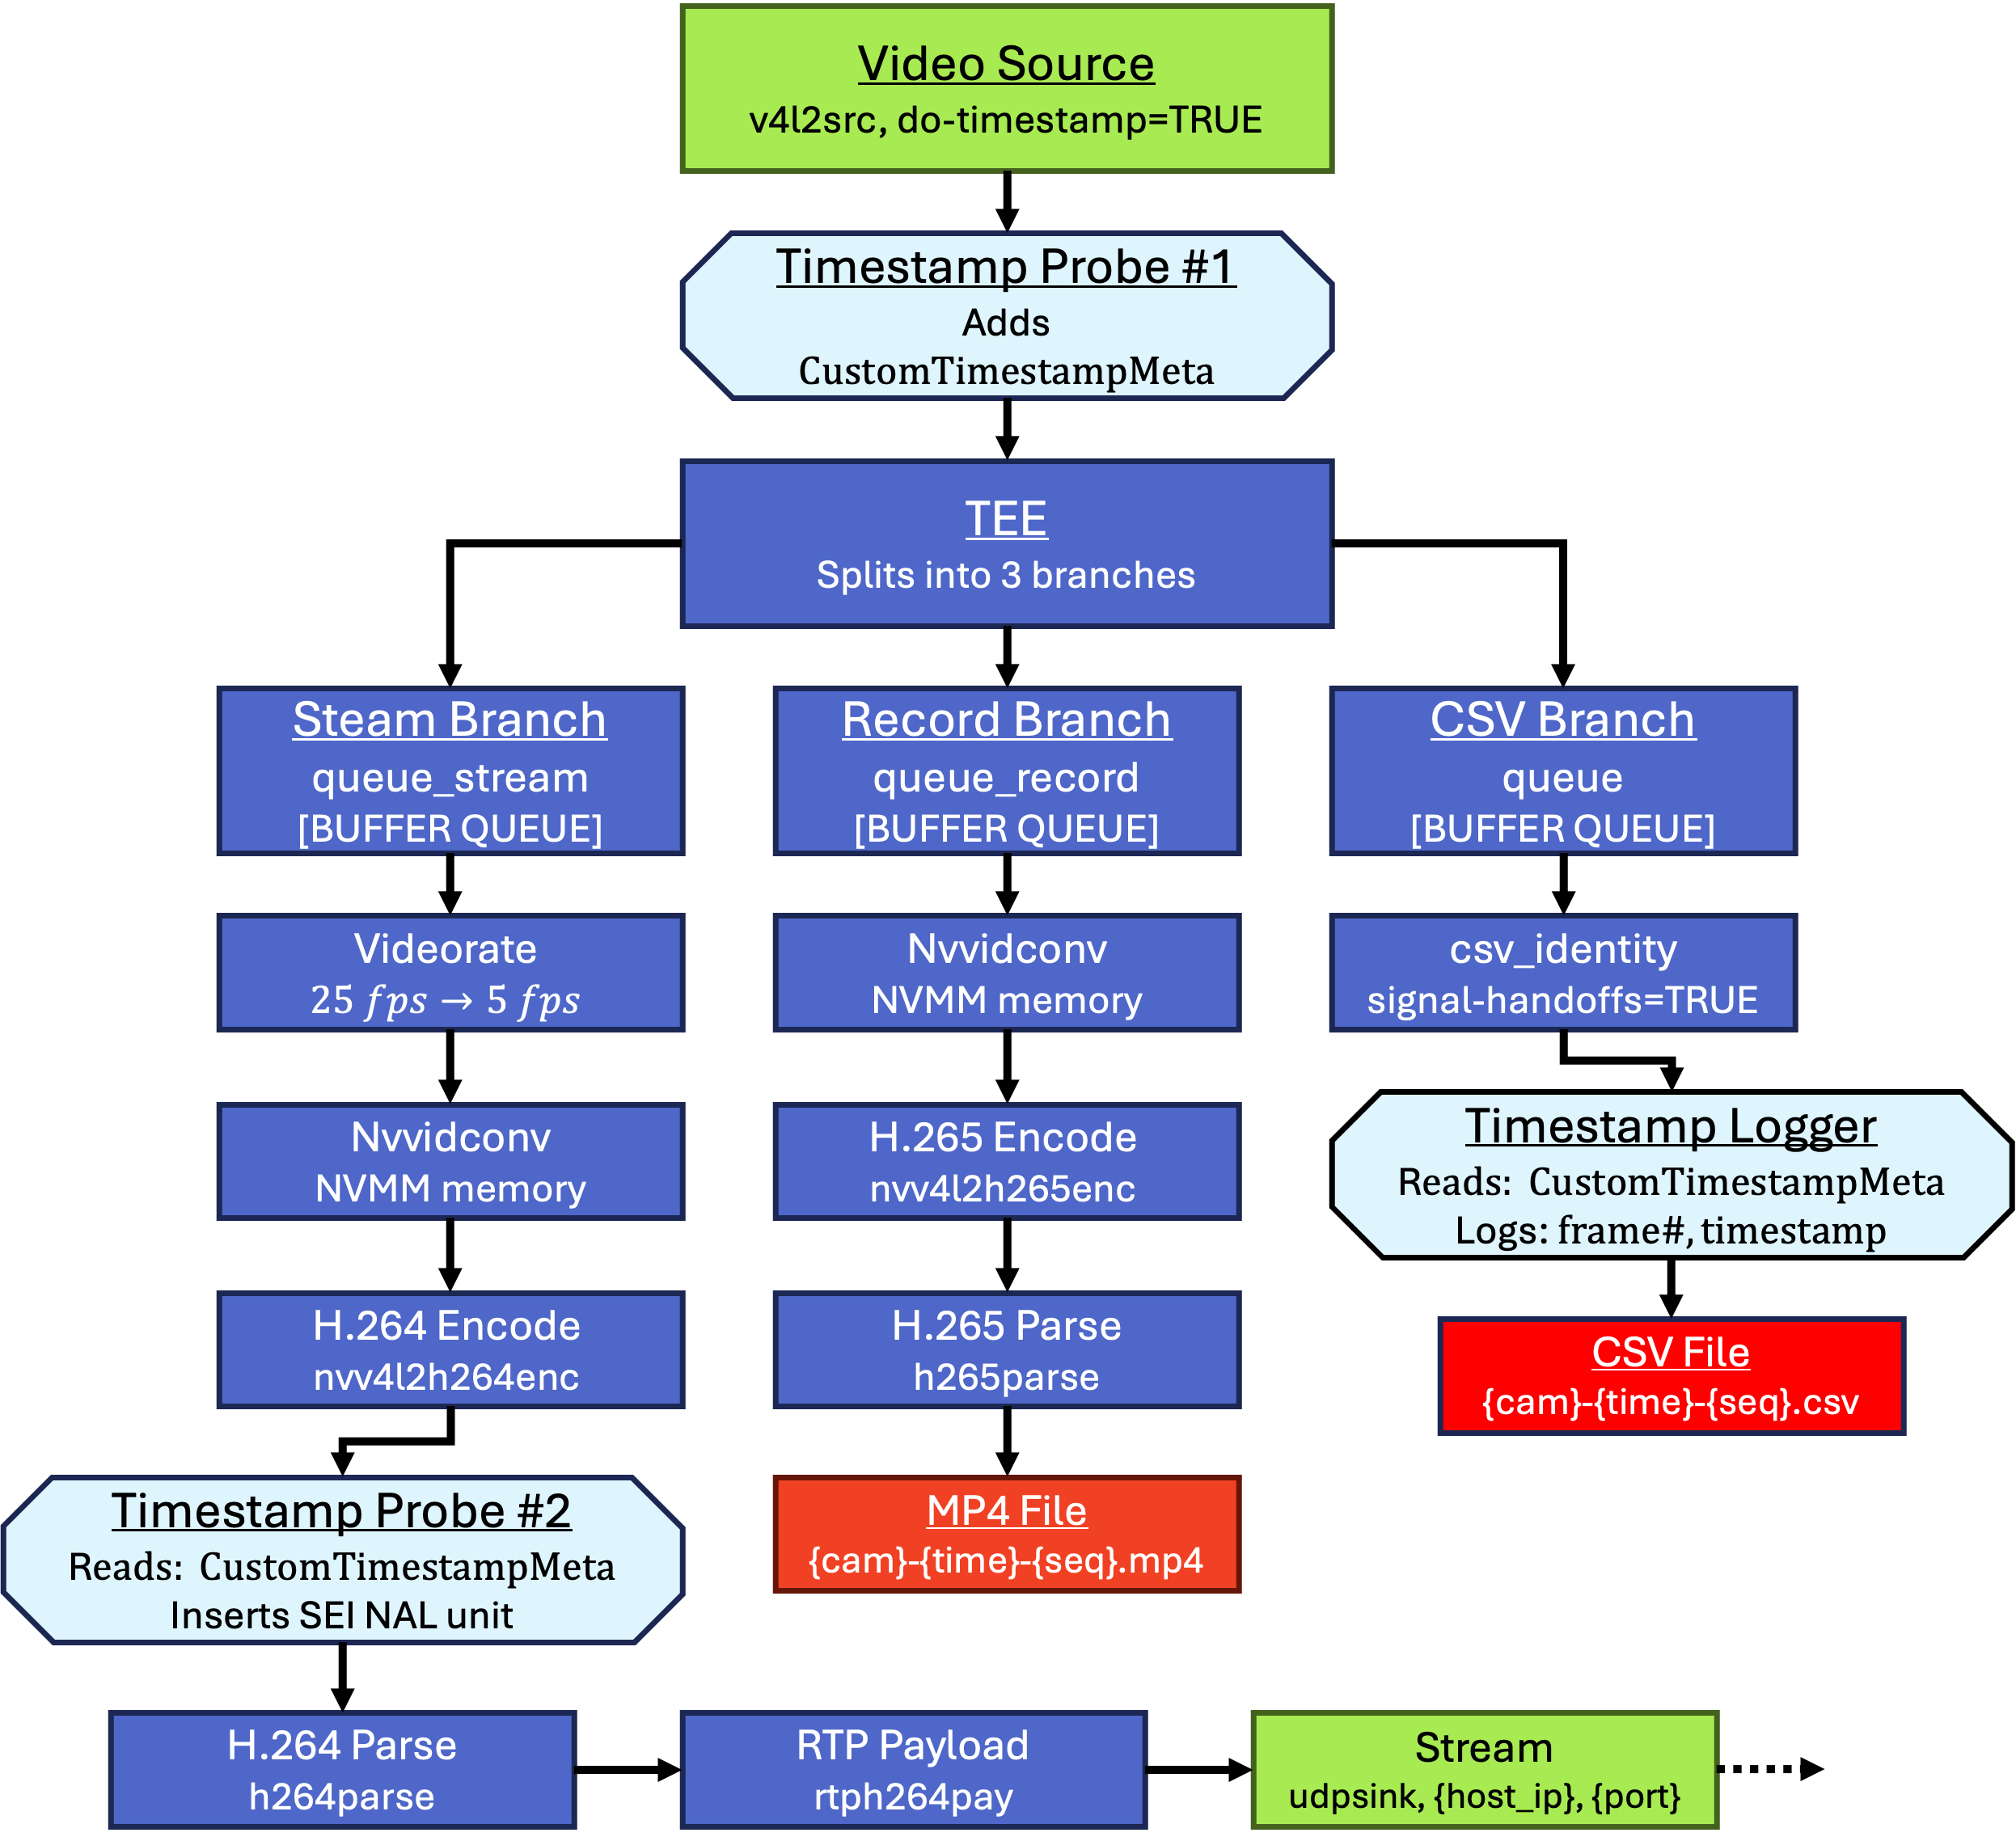
\includegraphics[width=0.95\textwidth]{Images/gstreamer_block.png}
\caption{Block diagram of the NVIDIA Jetson's video pipeline. Green rectangles represent video data entering or leaving the pipeline, while red rectangles indicate local file creation. Light-blue rectangles with chamfered corners denote timestamp acquisition and application operations within the pipeline.}
\label{fig_video_pipeline}
\end{figure}


% \chapter{test 2}

% \begin{figure}[htbp]
%        \centering
%        % TikZ Flowchart for GStreamer HDR Pipeline
% Drop-in code for Overleaf
% Requires: \usepackage{tikz}
%          \usetikzlibrary{shapes.geometric, arrows}

\tikzstyle{process} = [rectangle, minimum width=3cm, minimum height=1cm, text centered, draw=black, fill=white, text width=3cm]
\tikzstyle{timestamp} = [rectangle, minimum width=3cm, minimum height=1cm, text centered, draw=red, line width=1.5pt, fill=white, text width=3cm]
\tikzstyle{queue} = [rectangle, minimum width=2.5cm, minimum height=0.8cm, text centered, draw=blue, line width=1.2pt, fill=white, text width=2.5cm]
\tikzstyle{output} = [rectangle, minimum width=2.5cm, minimum height=1cm, text centered, draw=green!60!black, line width=1.2pt, fill=white, text width=2.5cm, rounded corners]
\tikzstyle{decision} = [diamond, minimum width=2cm, minimum height=1cm, text centered, draw=black, fill=white, aspect=2]
\tikzstyle{arrow} = [thick,->,>=stealth]

\begin{tikzpicture}[node distance=2cm]

% Source
\node (source) [process] {\textbf{v4l2src / videotestsrc} \\ YUY2, 2880x1860@60fps \\ do-timestamp=TRUE};

% Timestamp Probe 1
\node (ts1) [timestamp, below of=source] {\textbf{TIMESTAMP PROBE \#1} \\ timestamp\_probe\_cb \\ Adds CustomTimestampMeta \\ gettimeofday() $\rightarrow$ ms};

% Tee
\node (tee) [decision, below of=ts1, yshift=-0.5cm] {\textbf{TEE (Splits 3x)}};

% Stream Branch (left)
\node (qs) [queue, below of=tee, xshift=-8cm, yshift=-1.5cm] {\textbf{queue\_stream} \\ {[BUFFER QUEUE]}};
\node (vr) [process, below of=qs] {\textbf{videorate} \\ 60fps $\rightarrow$ 5fps};
\node (nvc1) [process, below of=vr] {\textbf{nvvidconv} \\ YUY2 $\rightarrow$ I420 \\ NVMM memory};
\node (h264e) [process, below of=nvc1] {\textbf{nvv4l2h264enc} \\ H264 encode \\ bitrate=calc \\ insert-sps-pps=true};
\node (sei) [timestamp, below of=h264e] {\textbf{TIMESTAMP PROBE \#2} \\ sei\_insert\_probe\_cb \\ Reads CustomTimestampMeta \\ Inserts SEI NAL unit};
\node (h264p) [process, below of=sei] {\textbf{h264parse} \\ Parse H264 stream};
\node (rtp) [process, below of=h264p] {\textbf{rtph264pay} \\ RTP payload \\ config-interval=1 \\ mtu=1400};
\node (udp) [output, below of=rtp] {\textbf{udpsink} \\ host=201.7.90.18 \\ port=5603 \\ sync=false};

% Record Branch (middle)
\node (qr) [queue, below of=tee, yshift=-1.5cm] {\textbf{queue\_record} \\ {[BUFFER QUEUE]}};
\node (nvc2) [process, below of=qr] {\textbf{nvvidconv} \\ YUY2 $\rightarrow$ I420 \\ NVMM memory};
\node (h265e) [process, below of=nvc2] {\textbf{nvv4l2h265enc} \\ H265 encode \\ bitrate=80Mbps \\ iframeinterval=1};
\node (h265p) [process, below of=h265e] {\textbf{h265parse} \\ Parse H265 \\ byte-stream};
\node (split) [output, below of=h265p, yshift=-1cm] {\textbf{splitmuxsink} \\ muxer=qtmux \\ Split @120s \\ /mnt/logs/hdr-0/ \\ hdr-0-\{time\}-\{n\}.mp4};

% CSV Branch (right)
\node (qc) [queue, below of=tee, xshift=8cm, yshift=-1.5cm] {\textbf{queue} \\ {[BUFFER QUEUE]}};
\node (id) [process, below of=qc] {\textbf{identity} \\ csv\_identity \\ signal-handoffs=true};
\node (csv) [timestamp, below of=id] {\textbf{TIMESTAMP LOGGER} \\ csv\_handoff\_handler \\ Reads CustomTimestampMeta \\ Logs: frame\#,timestamp};
\node (csvf) [output, below of=csv, xshift=-2.5cm, yshift=-0.5cm] {\textbf{CSV Files} \\ /mnt/logs/hdr-0/ \\ hdr-0-\{time\}-\{n\}.csv \\ Split @120s};
\node (fake) [output, below of=csv, xshift=2.5cm, yshift=-0.5cm] {\textbf{fakesink} \\ discard};

% Arrows
\draw [arrow] (source) -- (ts1);
\draw [arrow] (ts1) -- node[anchor=east, xshift=-0.3cm] {[BUFFER + Metadata]} (tee);

% Stream branch arrows
\draw [arrow] (tee) -| node[anchor=south, yshift=0.3cm, xshift=-4cm] {Stream Branch} (qs);
\draw [arrow] (qs) -- (vr);
\draw [arrow] (vr) -- (nvc1);
\draw [arrow] (nvc1) -- (h264e);
\draw [arrow] (h264e) -- (sei);
\draw [arrow] (sei) -- node[anchor=east, xshift=-0.3cm] {[H264 + SEI NAL]} (h264p);
\draw [arrow] (h264p) -- (rtp);
\draw [arrow] (rtp) -- node[anchor=east, xshift=-0.3cm] {[RTP Packets]} (udp);

% Record branch arrows
\draw [arrow] (tee) -- node[anchor=east, xshift=-0.3cm] {Record Branch} (qr);
\draw [arrow] (qr) -- (nvc2);
\draw [arrow] (nvc2) -- (h265e);
\draw [arrow] (h265e) -- (h265p);
\draw [arrow] (h265p) -- (split);

% CSV branch arrows
\draw [arrow] (tee) -| node[anchor=south, yshift=0.3cm, xshift=4cm] {CSV Branch} (qc);
\draw [arrow] (qc) -- (id);
\draw [arrow] (id) -- (csv);
\draw [arrow] (csv) -- (csvf);
\draw [arrow] (csv) -- (fake);

\end{tikzpicture}

%        \caption{GStreamer pipeline architecture for HDR camera streaming, 
%                 recording, and timestamp logging.}
%        \label{fig:hdr_pipeline}
%    \end{figure}


\end{document}